
\documentclass[aspectratio=169]{beamer}

% --------------------------------------------------
% Paquetes
% --------------------------------------------------
\usepackage[utf8]{inputenc}
\usepackage[T1]{fontenc}
\usepackage[spanish,es-nodecimaldot]{babel}
\usepackage{amsmath}
\usepackage{amssymb}
\usepackage{booktabs}
\usepackage{tikz}
\usepackage{graphicx}
\usepackage{xcolor}

\usetikzlibrary{
    arrows.meta,
    positioning,
    shapes.geometric,
    fit,
    backgrounds
}

% --------------------------------------------------
% Tema
% --------------------------------------------------
\usetheme{Madrid}
\usecolortheme{beaver}



%\usepackage[backend=biber,maxcitenames=50,maxbibnames=50,sorting=ydmdddnt]{biblatex}
\usepackage[backend=biber,maxcitenames=50,maxbibnames=50,sorting=none]{biblatex}






%\renewrobustcmd{\mkbibfootnote}{\normalsize\footnotemark\footnotetext}
\setbeamerfont{footnote}{size=\tiny}






\newcommand{\ArchivoPrincipal}{Todos}
\newcommand{\ArchivoSecundario}{Bibliografia}


%Append keywords to identify different bibliography entries.
\DeclareSourcemap{
  \maps[datatype=bibtex, overwrite]{
    \map{
      \perdatasource{\ArchivoPrincipal.bib}
      \step[fieldset=KEYWORDS, fieldvalue=primary, append]
    }
    \map{
      \perdatasource{\ArchivoSecundario.bib}
      \step[fieldset=KEYWORDS, fieldvalue=secundary, append]
    }    
  }
}


\addbibresource{\ArchivoPrincipal.bib}
\addbibresource{\ArchivoSecundario.bib}



% --------------------------------------------------
% Información
% --------------------------------------------------
\title[IA en dispositivos móviles]
      {Integración de Inteligencia Artificial en Aplicaciones Móviles}

\subtitle{Relación entre proyectos de investigación y aplicaciones inteligentes}

\author{Marco Aurelio Nuño-Maganda}

\institute[UPV]{Universidad Politécnica de Victoria\\ Laboratorio de Sistemas Inteligentes \\
mnunom@upv.edu.mx  \vspace{.25cm} }

\date{Octubre de 2026}

% --------------------------------------------------
% Comandos
% --------------------------------------------------
\newcommand{\ia}{Inteligencia Artificial}
\newcommand{\ondevice}{\textit{on-device}}

% A HUEVO EN TODOS!!!
\newcommand{\Folder}{YYY}
\newcommand{\EntradaBibtex}{XXX}

 \AtBeginSection[]
{
    \begin{frame}
        \frametitle{Contenido}
        \tableofcontents[currentsection]
    \end{frame}
}

\usepackage{tikz}
\usetikzlibrary{positioning}

% --------------------------------------------------
% Documento
% --------------------------------------------------
\begin{document}

% --------------------------------------------------
% Portada
% --------------------------------------------------
\begin{frame}
    \titlepage
\end{frame}

\frame{
\frametitle{Contenido}
\tableofcontents
}


\section{Introducción}
% ==================================================
% ¿QUÉ ES LA INTELIGENCIA ARTIFICIAL?
% ==================================================
\begin{frame}
\frametitle{¿Qué es la Inteligencia Artificial?}

\begin{block}{Definición}
La \textbf{Inteligencia Artificial (IA)} es el campo de la computación
que desarrolla sistemas capaces de realizar tareas que normalmente
requieren capacidades asociadas con la inteligencia humana.
\end{block}

\vspace{0.15cm}

\begin{columns}[T]

\column{0.70\textwidth}

\textbf{Capacidades de la IA}

\begin{itemize}
    \item \textbf{Percibir:} interpretar imágenes, audio y sensores.
    \item \textbf{Aprender:} identificar patrones a partir de datos.
    \item \textbf{Razonar:} analizar información y establecer relaciones.
    \item \textbf{Predecir:} estimar resultados o comportamientos.
    \item \textbf{Decidir:} seleccionar acciones con base en la información.
\end{itemize}

\begin{alertblock}{Idea clave}
\centering
\textbf{\tiny La IA permite transformar datos en conocimiento, predicciones
o decisiones para resolver problemas.}
\end{alertblock}


\column{0.30\textwidth}

\begin{center}

\begin{tikzpicture}[
    thick,scale=1, every node/.style={scale=0.65},
    node distance=0.45cm,
    box/.style={
        draw,
        rounded corners,
        minimum width=3.0cm,
        minimum height=0.65cm,
        align=center
    },
    arrow/.style={-{Latex}, thick}
]

\node[box] (data) {Datos\\e información};

\node[box, below=of data] (ai) {\textbf{Modelo de IA}};

\node[box, below=of ai] (result) {Predicción\\o decisión};

\node[box, below=of result] (action) {Acción\\o respuesta};

\draw[arrow] (data) -- (ai);
\draw[arrow] (ai) -- (result);
\draw[arrow] (result) -- (action);

\end{tikzpicture}

\end{center}

\end{columns}

\vspace{0.15cm}


\end{frame}



% ==================================================
% ¿QUÉ ES LA VISIÓN POR COMPUTADORA?
% ==================================================
\begin{frame}
\frametitle{¿Qué es la Visión por Computadora?}

\begin{block}{Definición}
La \textbf{Visión por Computadora (Computer Vision)} es un área de la
Inteligencia Artificial que permite a los sistemas computacionales
\textbf{analizar, interpretar y comprender información visual}.
\end{block}

\vspace{0.15cm}

\begin{columns}[T]

\column{0.75\textwidth}

\textbf{¿Qué puede hacer?}

\begin{itemize}
    \item \textbf{Detectar} objetos y personas.
    \item \textbf{Clasificar} imágenes.
    \item \textbf{Segmentar} regiones de interés.
    %\item \textbf{Reconocer} patrones y características.
    \item \textbf{Seguir} objetos y movimientos.
    \item \textbf{Estimar} posiciones y estructuras 3D.
\end{itemize}



%\begin{alertblock}{Idea clave}
%\centering
%\textbf{\tiny La Visión por Computadora transforma información visual
%en información que una máquina puede utilizar para comprender
%su entorno y tomar decisiones.}
%\end{alertblock}


\column{0.25\textwidth}

\begin{center}

\begin{tikzpicture}[
    thick,scale=1, every node/.style={scale=0.55},
    node distance=0.25cm,
    box/.style={
        draw,
        rounded corners,
        minimum width=3.0cm,
        minimum height=0.55cm,
        align=center
    },
    arrow/.style={-{Latex}, thick}
]

\node[box] (image) {Imagen / Video};

\node[box, below=of image] (processing)
    {Procesamiento\\de imagen};

\node[box, below=of processing] (features)
    {Características\\visuales};

\node[box, below=of features] (ai)
    {\textbf{Modelo de IA}};

\node[box, below=of ai] (result)
    {Interpretación\\o decisión};

\draw[arrow] (image) -- (processing);
\draw[arrow] (processing) -- (features);
\draw[arrow] (features) -- (ai);
\draw[arrow] (ai) -- (result);

\end{tikzpicture}

\end{center}

\end{columns}

\begin{block}{}
\textbf{\tiny La Visión por Computadora transforma información visual en información que una máquina puede utilizar para comprender su entorno y tomar decisiones.}
\end{block}{}



\end{frame}
\end{document}


\begin{frame}{¿Qué es el Aprendizaje Automático?}
\small

\begin{block}{Definición}
El \textbf{aprendizaje automático} (\textit{Machine Learning, ML}) es una
rama de la Inteligencia Artificial que permite a los sistemas
\textbf{aprender patrones a partir de datos} y utilizarlos para realizar
predicciones o tomar decisiones, sin programar explícitamente cada regla.
\end{block}

\vspace{0.2cm}

\begin{columns}[T,onlytextwidth]
    \begin{column}{0.48\textwidth}
        \textbf{¿Cómo funciona?}
        \begin{enumerate}
            \item Se recopilan datos.
            \item Se entrena un modelo con esos datos.
            \item Se evalúa su desempeño.
            \item El modelo procesa nuevos datos y genera resultados.
        \end{enumerate}
    \end{column}

    \begin{column}{0.48\textwidth}
        \centering
        \begin{tikzpicture}[
            node distance=0.55cm,
            box/.style={
                draw, rounded corners, align=center,
                minimum width=3.4cm, minimum height=0.75cm,
                fill=blue!8
            },
            arrow/.style={->, thick}
        ]
            \node[box] (datos) {Datos de entrenamiento};
            \node[box, below=of datos, fill=orange!15]
                (modelo) {Algoritmo de aprendizaje};
            \node[box, below=of modelo, fill=green!12]
                (resultado) {Modelo entrenado};
            \node[box, below=of resultado, fill=purple!10]
                (pred) {Predicción o decisión};

            \draw[arrow] (datos) -- (modelo);
            \draw[arrow] (modelo) -- (resultado);
            \draw[arrow] (resultado) -- (pred);
        \end{tikzpicture}
    \end{column}
\end{columns}

\vspace{0.2cm}

\begin{alertblock}{Ejemplos en dispositivos móviles}
Reconocer objetos con la cámara, identificar gestos de la mano,
clasificar imágenes, reconocer voz y detectar actividades mediante sensores.
\end{alertblock}

\end{frame}


\begin{frame}
\frametitle{Realidad Aumentada}
%\begin{alertblock}{Realidad Aumentada}
\begin{center}
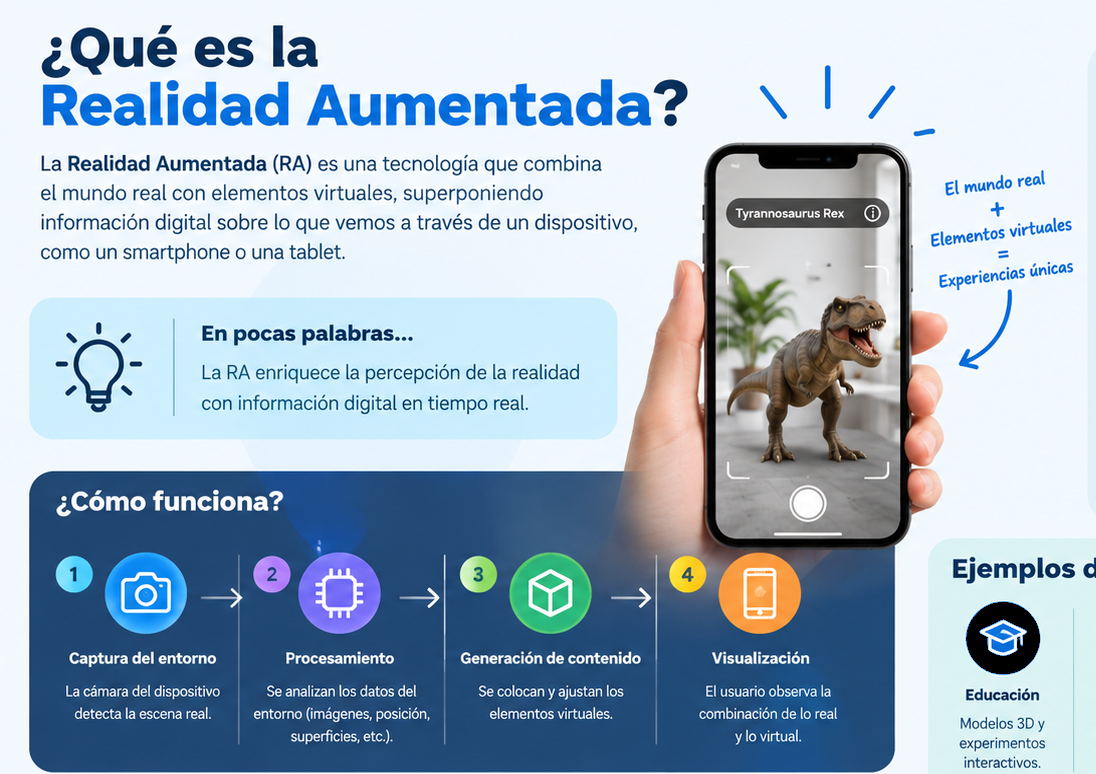
\includegraphics[width=0.65\linewidth]{00_IntroAR_VR/Infografia-Realidad-Aumentada-y-Aplicaciones.png}
\end{center}
%\end{alertblock}
\end{frame}



% ==================================================
% DIAPOSITIVA 1
% ==================================================
\begin{frame}
\frametitle{Inteligencia Artificial en Dispositivos Móviles}

\begin{block}{De las aplicaciones móviles tradicionales a sistemas inteligentes}
Los dispositivos Android integran cámaras, sensores, GPU y capacidad de cómputo suficiente para ejecutar modelos de \ia.
\end{block}

\vspace{0.2cm}

\begin{columns}[T]

\column{0.48\textwidth}

\textbf{La combinación de:}

\begin{itemize}
    \item Inteligencia Artificial
    \item Visión por computadora
    \item Sensores
    \item Realidad Aumentada
\end{itemize}

\column{0.48\textwidth}

\textbf{Permite:}

\begin{itemize}
    \item Reducir la dependencia de servidores.
    \item Disminuir la latencia.
    \item Mejorar la privacidad.
    \item Operar sin conexión permanente.
\end{itemize}

\end{columns}

\vspace{0.35cm}

\begin{center}
\begin{tikzpicture}[
    node distance=0.5cm,
    box/.style={
        draw,
        rounded corners,
        minimum width=2.8cm,
        minimum height=0.7cm,
        align=center
    },
    arrow/.style={-{Latex}, thick}
]

\node[box] (p) {Percepción};
\node[box, right=of p] (i) {Inteligencia};
\node[box, right=of i] (in) {Interacción};
\node[box, right=of in] (a) {Aplicación};

\draw[arrow] (p) -- (i);
\draw[arrow] (i) -- (in);
\draw[arrow] (in) -- (a);

\end{tikzpicture}
\end{center}

\end{frame}




\section{Herramientas}


% ==================================================
% HERRAMIENTAS DE IA: VISIÓN, VOZ Y MODELOS
% ==================================================
\begin{frame}
\frametitle{Herramientas de IA: Visión, Voz y Modelos}

%\small

%\begin{columns}[T]

% --------------------------------------------------
% VISIÓN POR COMPUTADORA
% --------------------------------------------------
%\column{0.49\textwidth}

\begin{block}{Visión por Computadora}
\begin{itemize}
    \item \textbf{OpenCV:} procesamiento de imágenes,
    filtros, geometría y seguimiento de objetos.

    \item \textbf{MediaPipe:} detección de manos,
    rostros, pose y puntos característicos.

    \item \textbf{CameraX:} integración de la cámara
    Android con el análisis de imágenes en tiempo real.
\end{itemize}
\end{block}





% --------------------------------------------------
% DESARROLLO DE MODELOS
% --------------------------------------------------
%\column{0.49\textwidth}

\begin{block}{Entrenamiento y Preparación}
\begin{itemize}
    \item \textbf{TensorFlow / Keras:}
    entrenamiento de redes neuronales y clasificación.

    \item \textbf{PyTorch:}
    desarrollo y entrenamiento de modelos de aprendizaje profundo.

\end{itemize}
\end{block}

\begin{block}{Integración en Android}
\begin{itemize}
    \item \textbf{Android Studio + Kotlin:}
    desarrollo de la aplicación móvil.

\end{itemize}
\end{block}

%\end{columns}

%\vspace{0.15cm}

\begin{center}
\begin{tikzpicture}[
    node distance=0.35cm,
    box/.style={
        draw,
        rounded corners,
        minimum height=0.6cm,
        minimum width=2.4cm,
        align=center,
        font=\small
    },
    arrow/.style={-{Latex}, thick}
]

\node[box] (data) {Cámara / Audio / Sensores};
\node[box, right=of data] (model) {Modelo o API de IA};
\node[box, right=of model] (app) {Aplicación Android};

\draw[arrow] (data) -- (model);
\draw[arrow] (model) -- (app);

\end{tikzpicture}
\end{center}

\end{frame}



% Diapositiva 1: Introducción a MediaPipe
\begin{frame}{¿Qué es MediaPipe?}
    \begin{itemize}
        \item Es una biblioteca de código abierto de Google para procesamiento de señales en tiempo real.
        \item Permite la implementación de modelos de Machine Learning en dispositivos móviles y de escritorio.
        \item Soporta múltiples plataformas como Android, iOS, y Python.
    \end{itemize}
    Flujo de Procesamiento:
    \begin{enumerate}
        \item Captura de datos desde una cámara o archivo.
        \item Procesamiento mediante el gráfico de MediaPipe.
        \item Obtención de resultados como coordenadas de puntos clave o segmentación.
    \end{enumerate}

\end{frame}

% Diapositiva 3: Soluciones preentrenadas
\begin{frame}{Soluciones preentrenadas de MediaPipe: Detección facial}
    Seguimiento de rasgos faciales para aplicaciones como realidad aumentada y reconocimiento facial.
     \begin{itemize}
        \item Utiliza una malla 3D con 468 puntos clave en el rostro.
        \item Permite el reconocimiento detallado de expresiones faciales y contornos.
        \item Funciona en tiempo real para aplicaciones como filtros de realidad aumentada y seguimiento facial.
        \item Proporciona una representación tridimensional sin necesidad de sensores de profundidad.
    \end{itemize}
    \begin{center}
        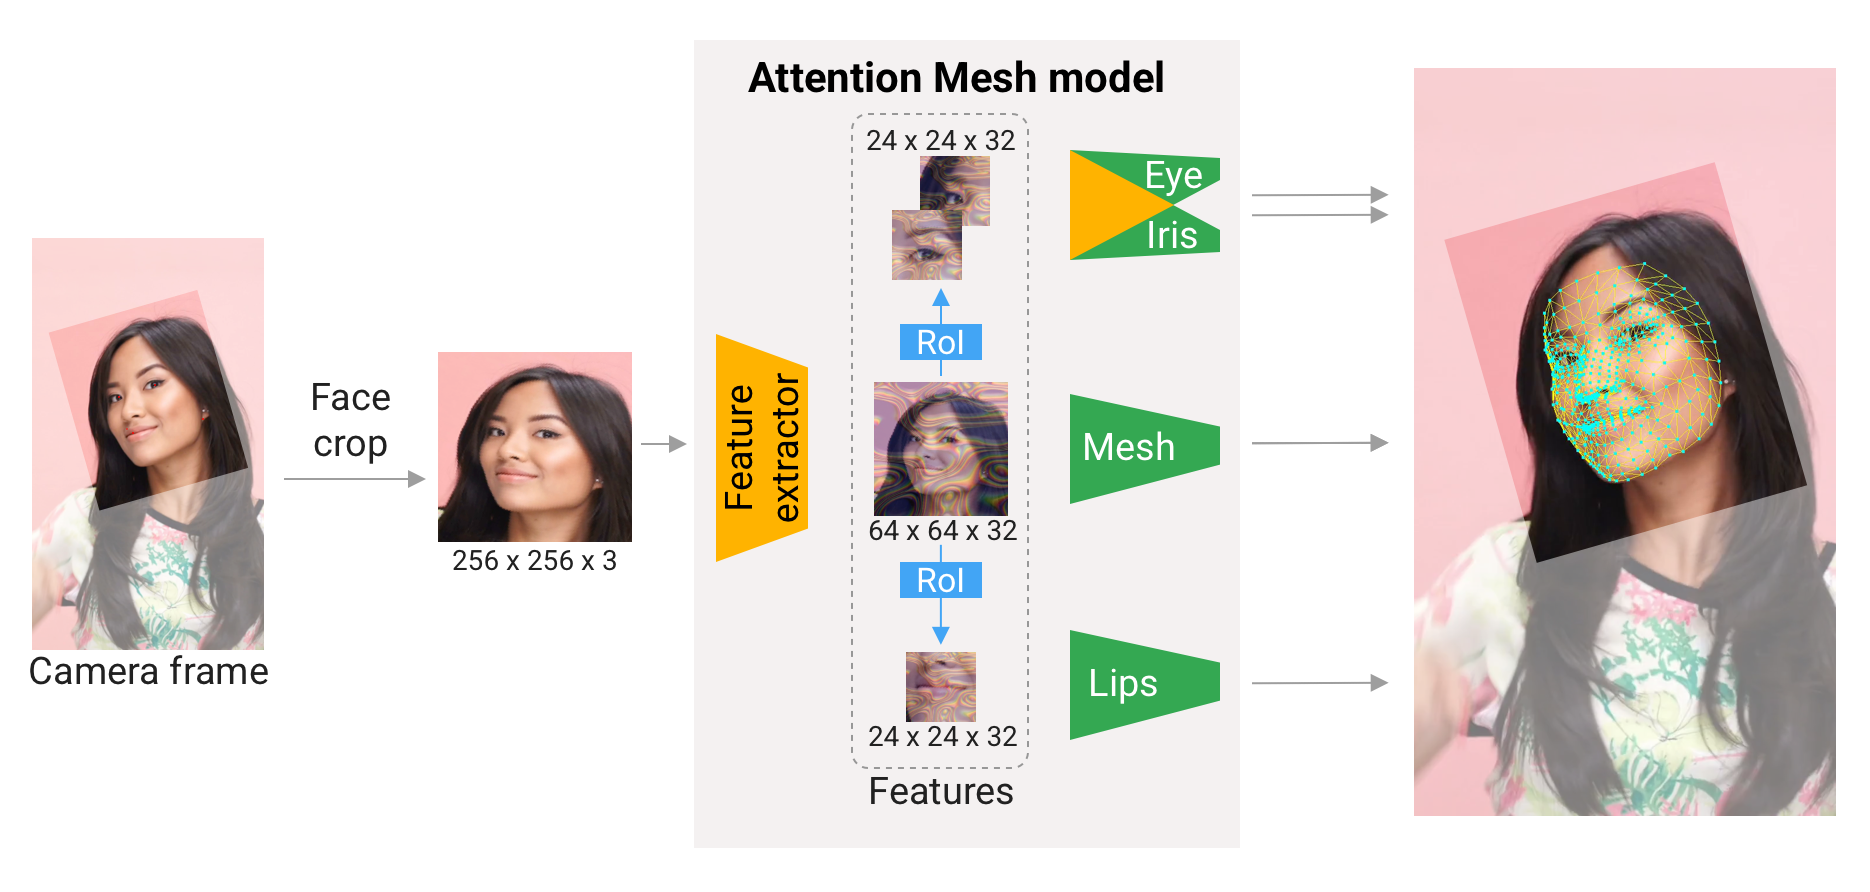
\includegraphics[width=0.6\linewidth]{01_MediaPipe/fase_mesh_detection.png}
    \end{center}
\end{frame}

\begin{frame}{Soluciones preentrenadas de MediaPipe: Detección de pose }
    Identificación de puntos clave en el cuerpo humano para análisis de movimiento.
    \begin{itemize}
        \item Utiliza modelos de aprendizaje profundo para identificar 33 puntos clave en el cuerpo humano.
        \item Procesa imágenes en tiempo real desde la cámara o archivos de video.
        \item Genera un esqueleto virtual basado en las coordenadas de los puntos detectados.
        \item Se emplea en aplicaciones como deportes, rehabilitación y realidad aumentada.
    \end{itemize}    
    \begin{center}
        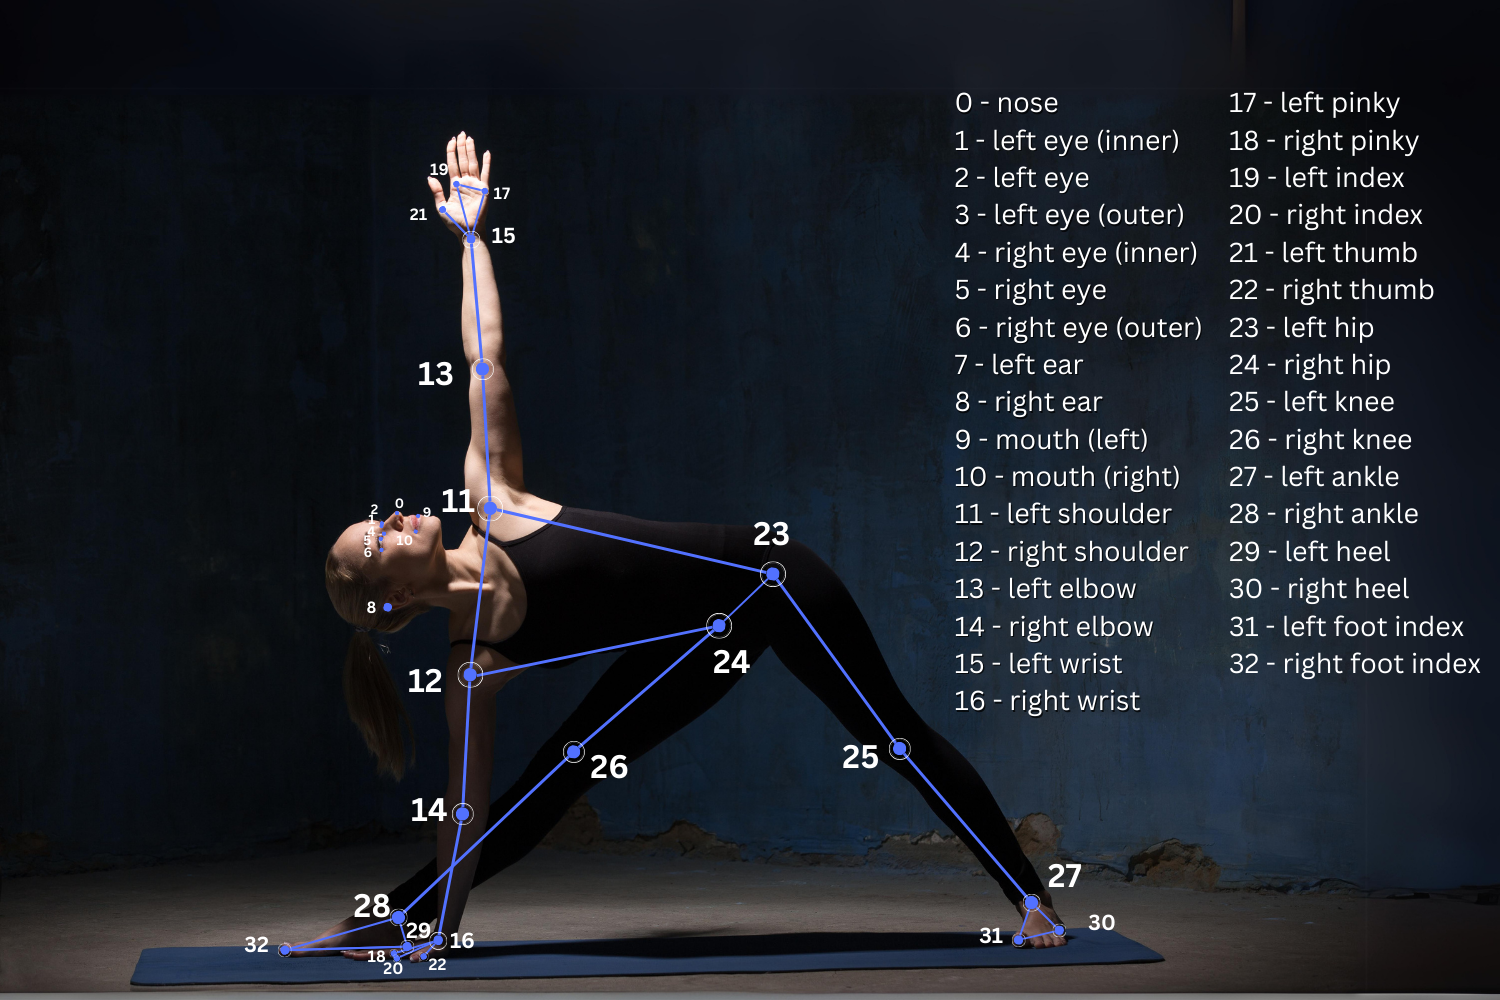
\includegraphics[width=0.5\linewidth]{01_MediaPipe/pose_landmarks.png}
    \end{center}
\end{frame}

\begin{frame}{Soluciones preentrenadas de MediaPipe: Detección de manos}
    Segmentación y seguimiento de manos en tiempo real para gestos y control por movimientos.
   \begin{itemize}
        \item Detecta 21 puntos clave en cada mano utilizando modelos de Machine Learning.
        \item Funciona en tiempo real, permitiendo el seguimiento preciso de los movimientos de la mano.
        \item Se utiliza en aplicaciones como control por gestos, realidad aumentada y comunicación en lenguaje de señas.
        \item Proporciona coordenadas tridimensionales sin necesidad de sensores adicionales.
    \end{itemize}
    \begin{center}
        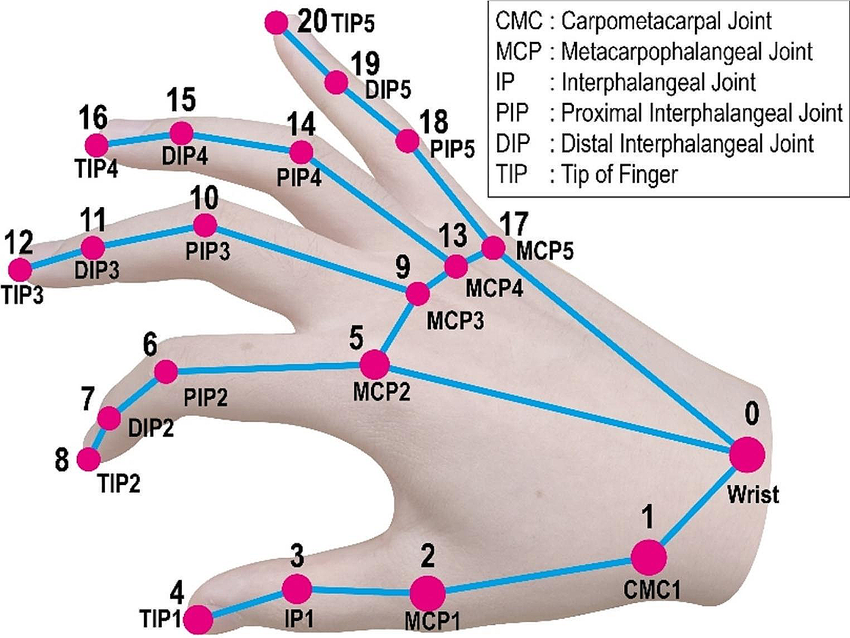
\includegraphics[width=0.30\linewidth]{01_MediaPipe/hand_landmarks.png}
    \end{center}
\end{frame}




% ==================================================
% GRÁFICOS 3D, REALIDAD AUMENTADA E IA
% ==================================================
\begin{frame}
\frametitle{Gráficos 3D, Realidad Aumentada e IA Móvil}
\begin{block}{OpenGL ES: Renderizado gráfico 3D}
\begin{itemize}
    \item Renderizado acelerado por GPU, Animaciones, geometría y texturas.
\end{itemize}
\end{block}

\begin{block}{Rajawali3D: Motor 3D para Android}
\begin{itemize}
    \item Simplifica escenas, cámaras, luces y materiales, facilita la creación de entornos 3D.
\end{itemize}
\end{block}


\begin{block}{ARCore: Percepción espacial}
\begin{itemize}
    \item Seguimiento de movimiento, detección de superficies y estimación de profundidad,
\end{itemize}   
\end{block}

\begin{block}{Sceneform: Desarrollo de experiencias de RA}
\begin{itemize}
    \item Facilita la integración de modelos 3D en aplicaciones Android.
\end{itemize}
\end{block}

\vspace{0.15cm}

\begin{center}
\begin{tikzpicture}[
    node distance=0.35cm,
    box/.style={
        draw,
        rounded corners,
        minimum width=2.25cm,
        minimum height=0.65cm,
        align=center,
        font=\scriptsize
    },
    arrow/.style={-{Latex}, thick}
]

\node[box] (sensor) {Cámara y sensores};
\node[box, right=of sensor] (ar) {ARCore / RA};
\node[box, right=of ar] (ai) {Modelo de IA};
\node[box, right=of ai] (render) {OpenGL ES / 3D};

\draw[arrow] (sensor) -- (ar);
\draw[arrow] (ar) -- (ai);
\draw[arrow] (ai) -- (render);

\end{tikzpicture}
\end{center}

%\begin{alertblock}{Aportación de la IA}
%La IA reconoce objetos, gestos o poses; las herramientas 3D y de RA
%permiten representar sus resultados e interactuar con ellos en el
%entorno real.
%\end{alertblock}

\end{frame}

\section{Proyectos}

\subsection{Reconocimiento de actividades y ubicaciones}

\renewcommand{\EntradaBibtex}{MarcoNuno_CongArbIng_2015_02_00}
\begin{frame}{\citetitle{\EntradaBibtex} \footnotemark[1] (1)}


%\subsection{Aprendizaje automático}
%\begin{frame}{\citetitle{MarcoNuno_CongArbIng_2015_02_00} \footnotemark (1) }
\begin{columns}
\begin{column}{0.4\textwidth}
		Componentes:
		\begin{itemize}
		\item Captura de datos del acelerómetro del teléfono
		\item Procesar los datos empleando algoritmos de ML previamente entrenados, para determinar el tipo de actividad llevada a cabo por el usuario
		\end{itemize}
\end{column}
\begin{column}{0.6\textwidth}  
    \begin{center}
     %%%%% this is a minipage, so \textwidth is already adjusted to the size of the column
     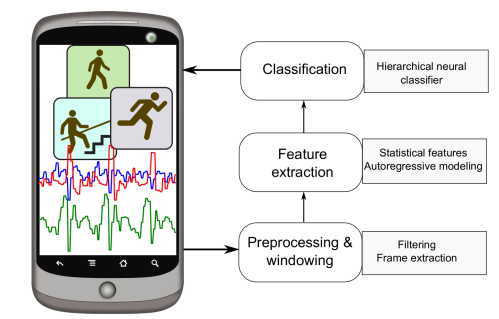
\includegraphics[width=0.8\textwidth]{Figs/DeteccionActividad1}
     \end{center}
\end{column}
\end{columns}
\footnotetext[1]{\fullcite{\EntradaBibtex}}
\end{frame}


\begin{frame}{\citetitle{\EntradaBibtex} (2)}
\begin{columns}
\begin{column}{0.40\textwidth}
		Componentes:
		\begin{itemize}
		\item Se empleo una red neuronal jerárquica
		\item Se midió el desempeño de la bateria y los tiempos de los principales pasos
		\end{itemize}
\begin{center}
     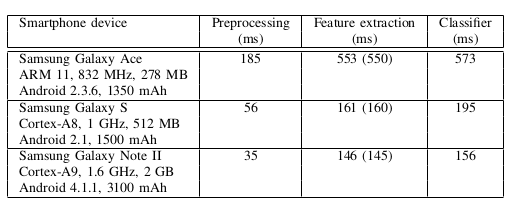
\includegraphics[width=0.7\textwidth]{Figs/DeteccionActividad3}
     
     \end{center}
\end{column}
\begin{column}{0.29\textwidth}  
    \begin{center}
     %%%%% this is a minipage, so \textwidth is already adjusted to the size of the column
     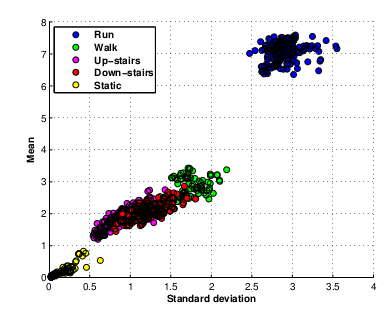
\includegraphics[width=0.97\textwidth]{Figs/DeteccionActividad2}
	%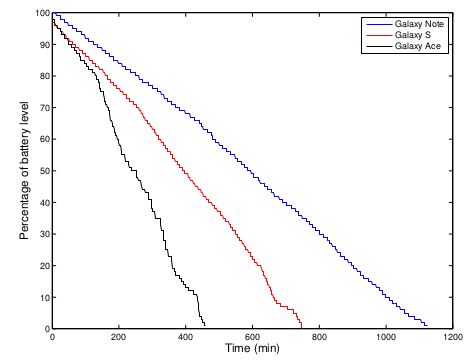
\includegraphics[width=0.7\textwidth]{Figs/DeteccionActividad4}

     \end{center}
\end{column}
\begin{column}{0.29\textwidth}  
    \begin{center}
     %%%%% this is a minipage, so \textwidth is already adjusted to the size of the column
     %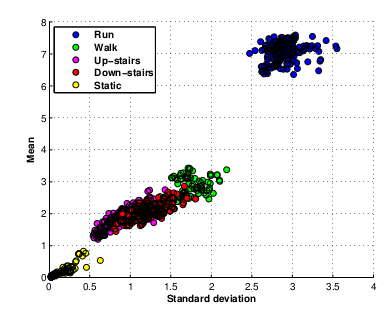
\includegraphics[width=0.7\textwidth]{Figs/DeteccionActividad2}
	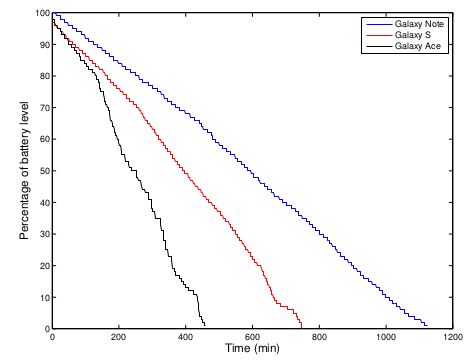
\includegraphics[width=0.97\textwidth]{Figs/DeteccionActividad4}

     \end{center}

\end{column}
\end{columns}
\end{frame}




\renewcommand{\EntradaBibtex}{MarcoNuno_Revista_2018_07_00}
\begin{frame}{\citetitle{\EntradaBibtex} \footnotemark[1] (1)}



%\begin{frame}{\citetitle{MarcoNuno_Revista_2018_07_00} \footnotemark (1)}
%\begin{block}{Sistema de Posicionamiento Interior \footnotemark (1)} 
\begin{columns}
\begin{column}{0.5\textwidth}
		\begin{itemize}
		\item Determinar la ubicación de personas/objetos móviles en interiores es un problema abierto
		\item Se propuso un sistema basado en ML, para procesar las intensidades de señal de los puntos de acceso y de esta forma poder conocer la ubicación de manera precisa
		\end{itemize}
\end{column}
\begin{column}{0.3\textwidth}  
    \begin{center}
     %%%%% this is a minipage, so \textwidth is already adjusted to the size of the column
     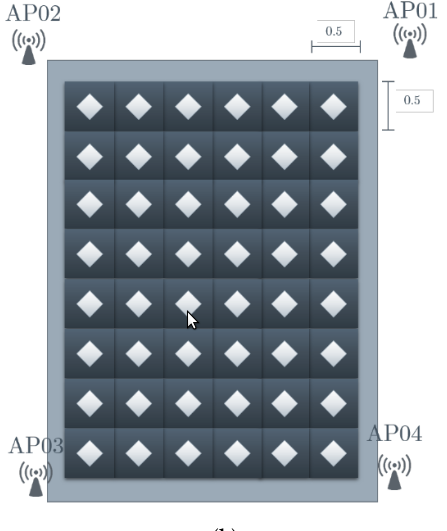
\includegraphics[width=0.85\textwidth]{Figs/IndoorPositionSystem2}
     \end{center}

\end{column}

\begin{column}{0.2\textwidth}  
    \begin{center}
     %%%%% this is a minipage, so \textwidth is already adjusted to the size of the column
     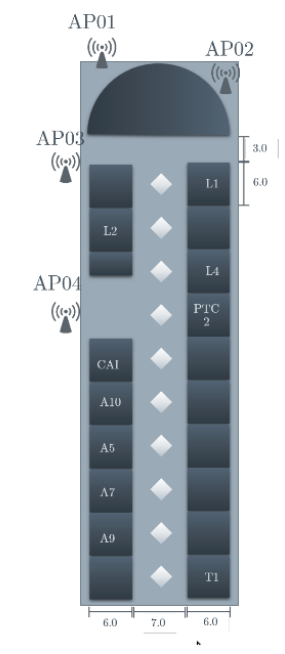
\includegraphics[width=0.8\textwidth]{Figs/IndoorPositionSystem1}
     \end{center}
\end{column}
\end{columns}
%\end{block} 
\footnotetext[1]{\fullcite{\EntradaBibtex}}
\end{frame}

\begin{frame}{\citetitle{\EntradaBibtex} (2)}
%\begin{block}{Sistema de Posicionamiento Interior (2)} 
\begin{columns}
\begin{column}{0.5\textwidth}
  \begin{center}
     %%%%% this is a minipage, so \textwidth is already adjusted to the size of the column
     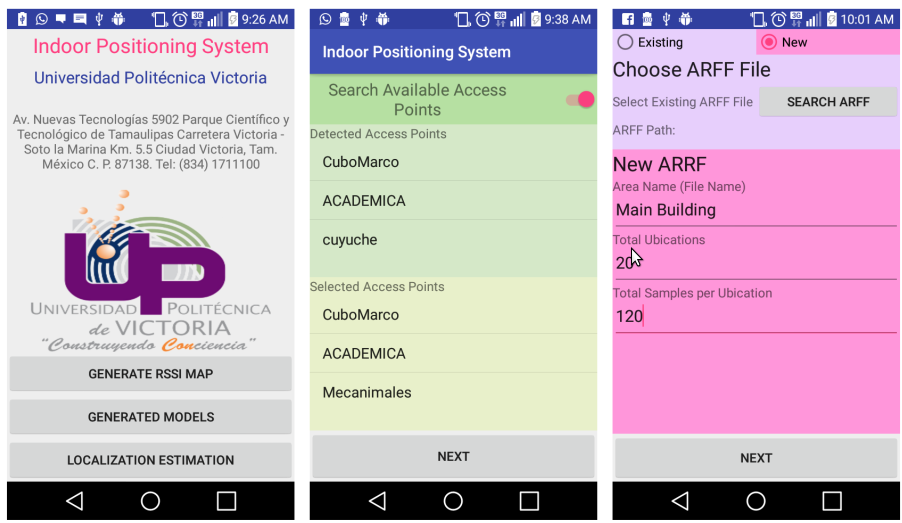
\includegraphics[width=0.95\textwidth]{Figs/IndoorPositionSystem3}
     %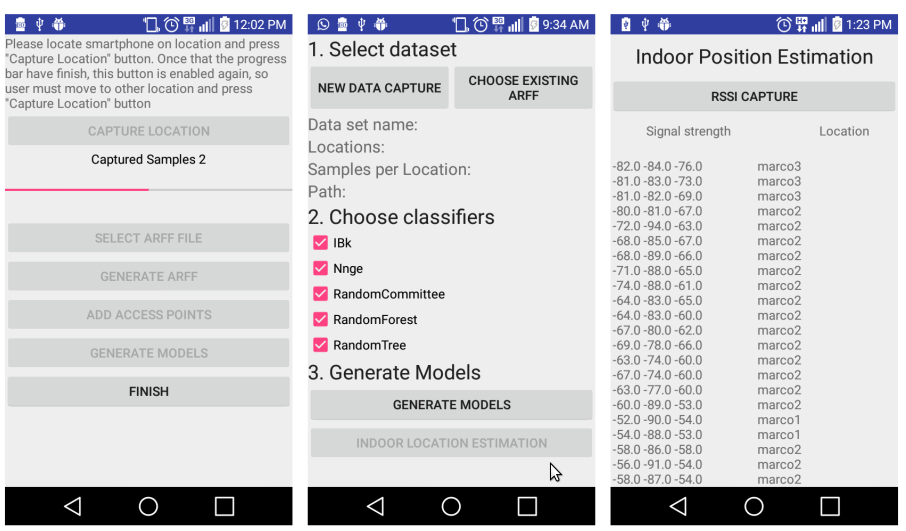
\includegraphics[width=0.5\textwidth]{Figs/IndoorPositionSystem4}
     \end{center}

\end{column}
\begin{column}{0.5\textwidth}
  \begin{center}
     %%%%% this is a minipage, so \textwidth is already adjusted to the size of the column
     %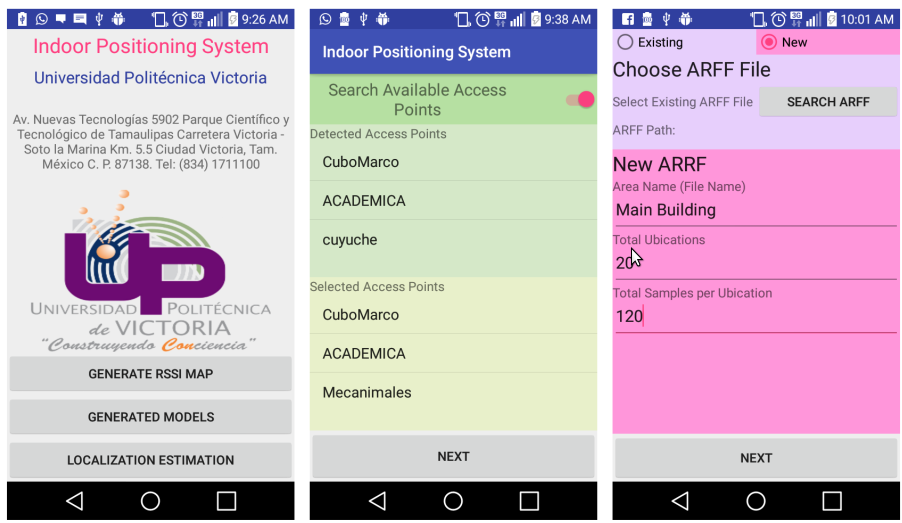
\includegraphics[width=0.5\textwidth]{Figs/IndoorPositionSystem3}
     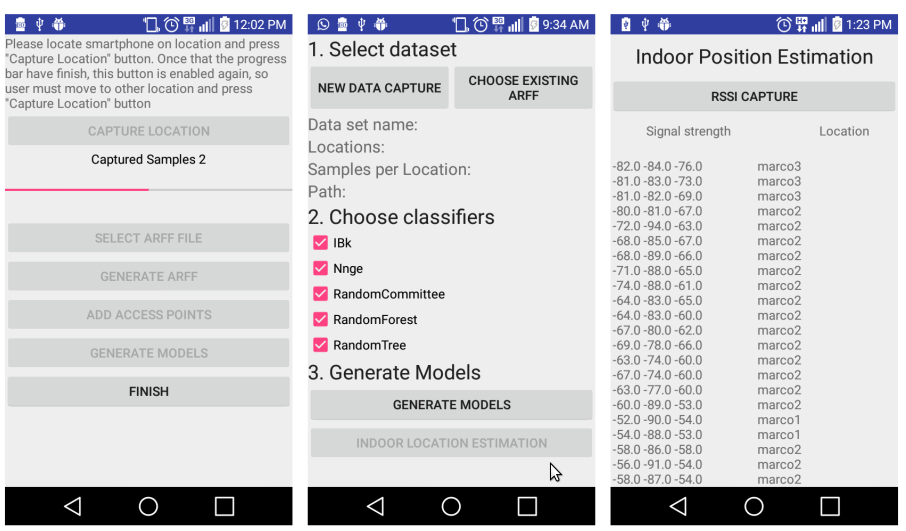
\includegraphics[width=0.95\textwidth]{Figs/IndoorPositionSystem4}
     \end{center}

\end{column}

\end{columns}



%\end{block} 
\end{frame}







\subsection{Reconocimiento basado en visión por computadora}





%\begin{frame}{\citetitle{MarcoNuno_CongArbEsp_2020_09_01} \footnotemark (1)}

\renewcommand{\EntradaBibtex}{MarcoNuno_CongArbEsp_2020_09_01}
\begin{frame}{\citetitle{\EntradaBibtex} \footnotemark[1] (1)}


\begin{block}{Detección de conductores autorizados \footnotemark } 
\begin{columns}
\begin{column}{1.0\textwidth}
Se propone un sistema montado en un teléfono inteligente que pueda:
	\begin{itemize}
\item Confirmar de manera continua la identidad de los ocupantes empleando la cámara frontal o posterior
\item Monitorear la ubicación del vehículo mediante el sensor GPS
\item Monitorear cuando el vehículo está en movimiento mediante los acelerómetros
\item Trabajar de manera independiente, conectado continuamente a la corriente y con conexión de datos propia para comunicación externa
	\end{itemize}
\end{column}
\end{columns}
\end{block} 
\footnotetext[1]{\fullcite{\EntradaBibtex}}
\end{frame}


\begin{frame}{\citetitle{\EntradaBibtex} (2)}
%\begin{block}{Detección de conductores autorizados (2)} 
\begin{columns}
\begin{column}{0.55\textwidth}
Fases de la ejecución:
	\begin{enumerate}
\item Enrolamiento: Los usuarios usan el automovil y sus rostros quedan guardados.
\item Prueba: Se reporta el ingreso de cualquier extraño.
	\end{enumerate}
Limitaciones:
	\begin{itemize}
\item Solo piloto, copiloto y tal vez pasajero viajando en el centro de la parte posterior.
\item Iluminación diurna.
\item Camuflaje en fase temprana.
	\end{itemize}

\end{column}
\begin{column}{0.45\textwidth}
\begin{center}
     %%%%% this is a minipage, so \textwidth is already adjusted to the size of the column
     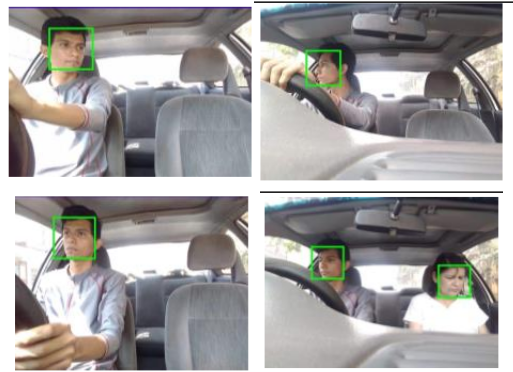
\includegraphics[width=0.99\textwidth]{Figs/ConductorAutorizado1}
     \end{center}
\end{column}

\end{columns}
%\end{block} 
\end{frame}





\renewcommand{\EntradaBibtex}{ProyectoLSM_2022}

\begin{frame}{\citetitle{\EntradaBibtex} \footnotemark[1] (1)}
\begin{columns}
\begin{column}{0.6\textwidth}
	\begin{itemize}
		\item Se propone una aplicación móvil que reconozca el lenguaje de señas mexicano (LSM)
        \item El equipo capturó videos de los diferentes gestos a clasificar (palabras comunes y letras del alfabeto)
        \item Se utilizó la libreria MediaPipe para la obtención de los marcadores de manos, torso y cabeza
        \item Se entrenó una Red Neuronal Convolucional
	\end{itemize}
\end{column}
\begin{column}{0.4\textwidth}  
\begin{center}
     \begin{tabular}{cc}

         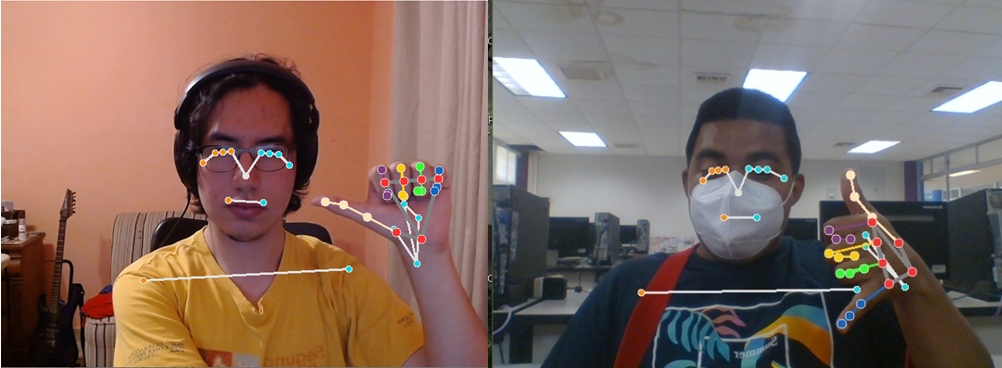
\includegraphics[width=0.98\textwidth]{2022_AplicacionLSM/figs/Diapositiva1.PNG}\\         
      \end{tabular}
\end{center}
\end{column} 
\end{columns} 
\footnotetext[1]{\fullcite{\EntradaBibtex}}
\end{frame}


\begin{frame}{\citetitle{\EntradaBibtex} (2)}
\begin{columns}
\begin{column}{0.6\textwidth}
Librerías utilizadas:
\begin{itemize}
        \item Tensorflow (PC) y Tensorflow-lite (Smartphone)
		\item MediPipe
	\end{itemize}
Para cada video:
\begin{itemize}
        \item Se normaliza la duración del video a una duración estándard
		\item Se entraen ubicaciones de los marcadores y se estiman angulos
		\item Se anexa al dataset para su posterior entrenamiento
	\end{itemize}
\end{column}
\begin{column}{0.4\textwidth}  
\begin{center}
     \begin{tabular}{c}
         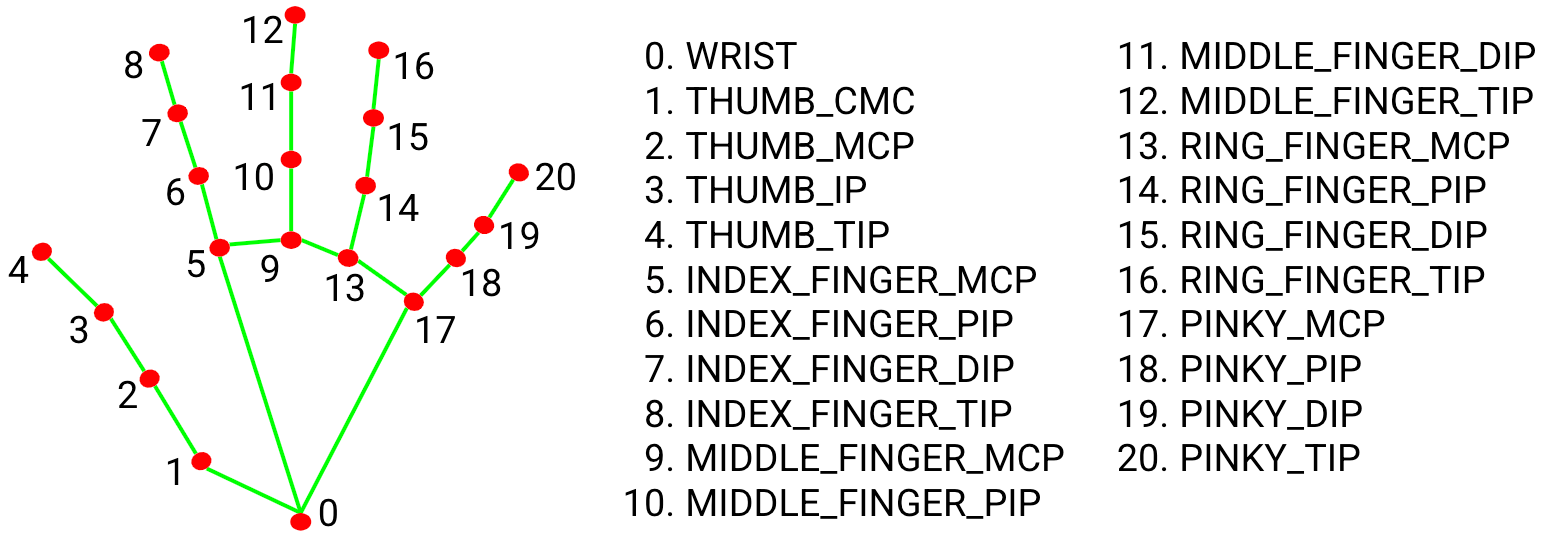
\includegraphics[width=0.98\textwidth]{2022_AplicacionLSM/figs/hand_landmarks.png}\\
          \end{tabular}
\end{center}
\end{column} 
\end{columns} 
\end{frame}

\begin{frame}{\citetitle{\EntradaBibtex} (3)}
Una vez entrenada la red, el modelo se incorpora a la aplicación
\begin{center}
 \begin{tabular}{cccc}
    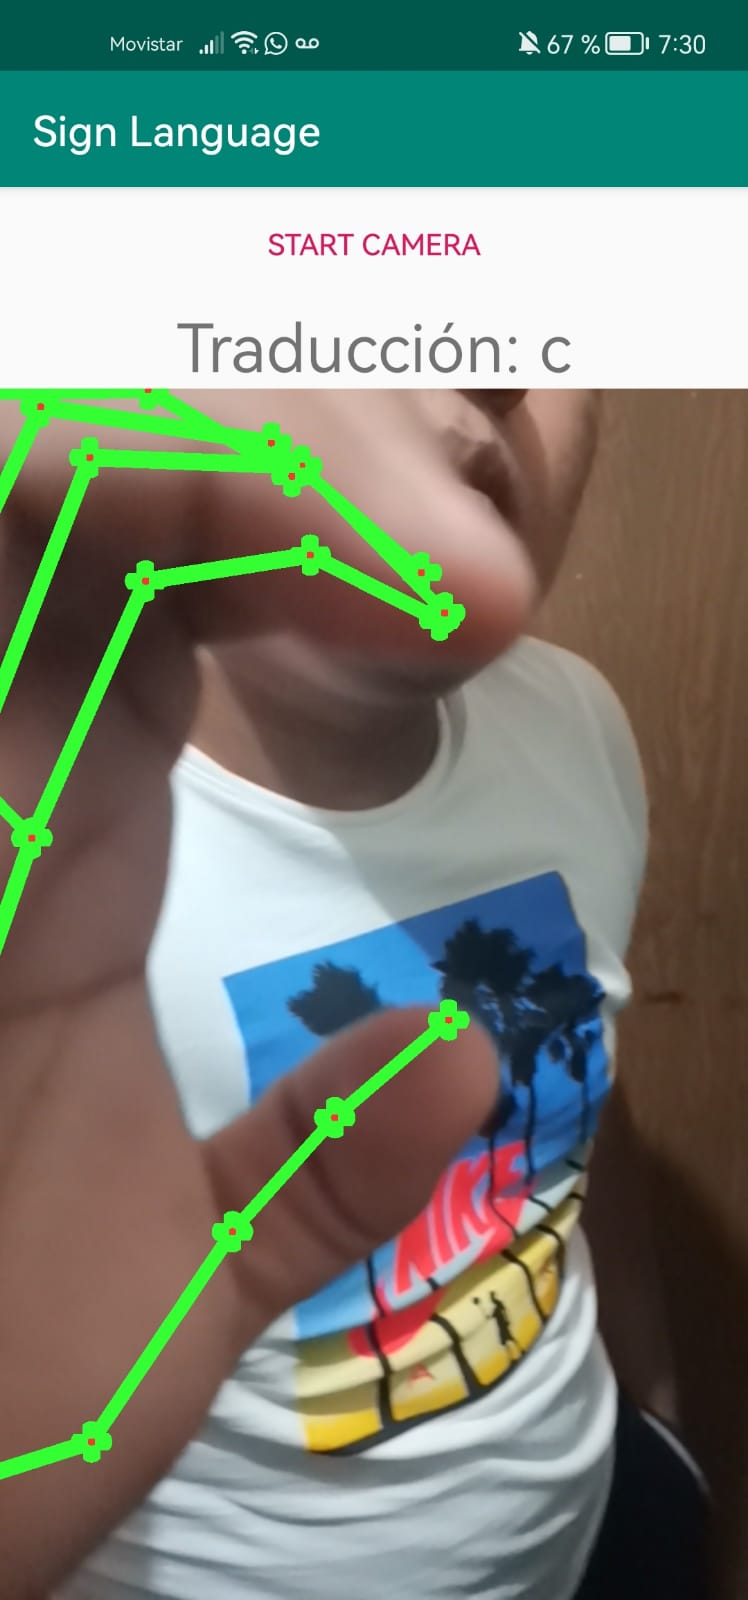
\includegraphics[width=0.16\textwidth]{2022_AplicacionLSM/figs/App1.jpeg}
    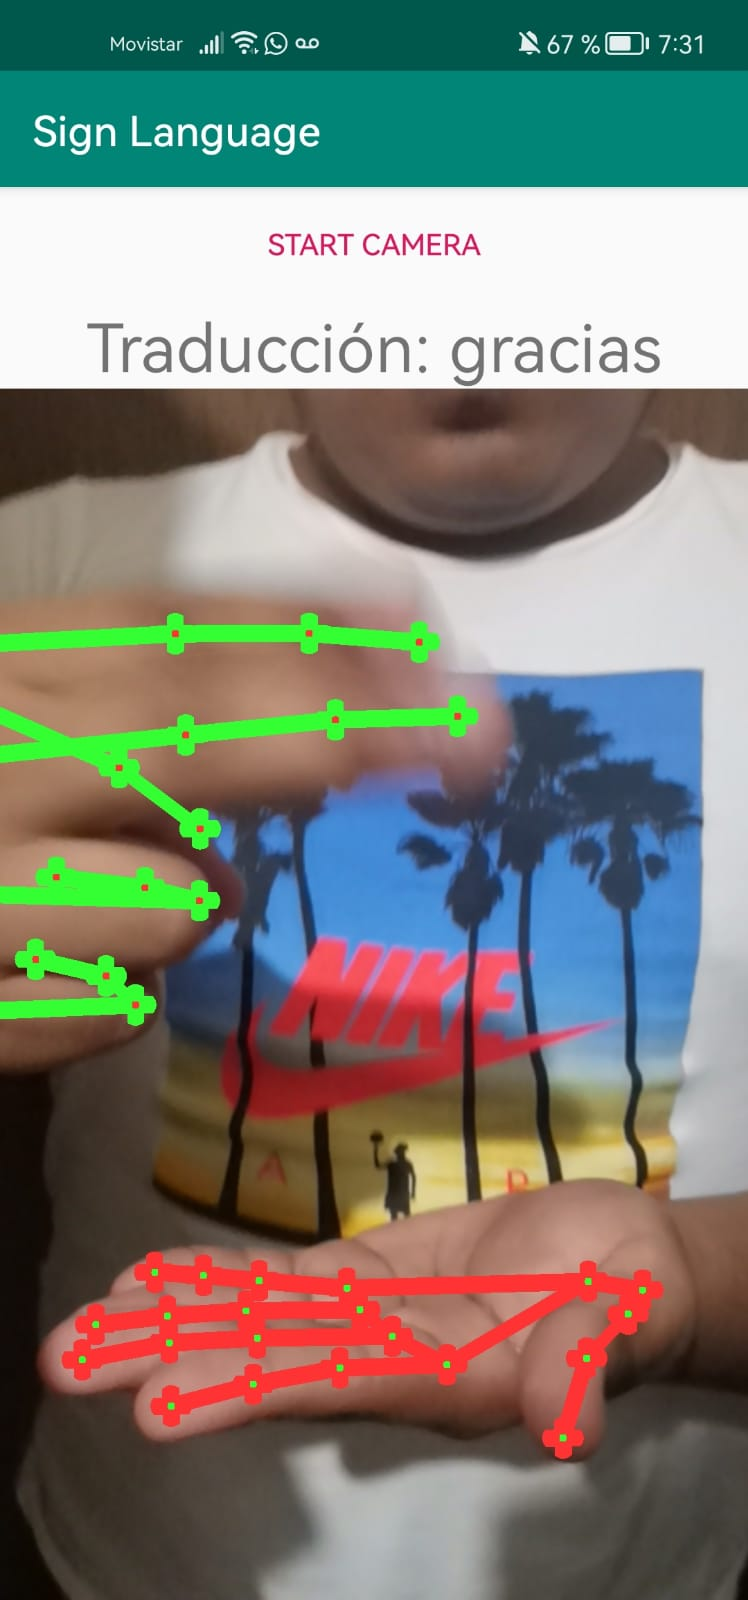
\includegraphics[width=0.16\textwidth]{2022_AplicacionLSM/figs/App2.jpeg}
    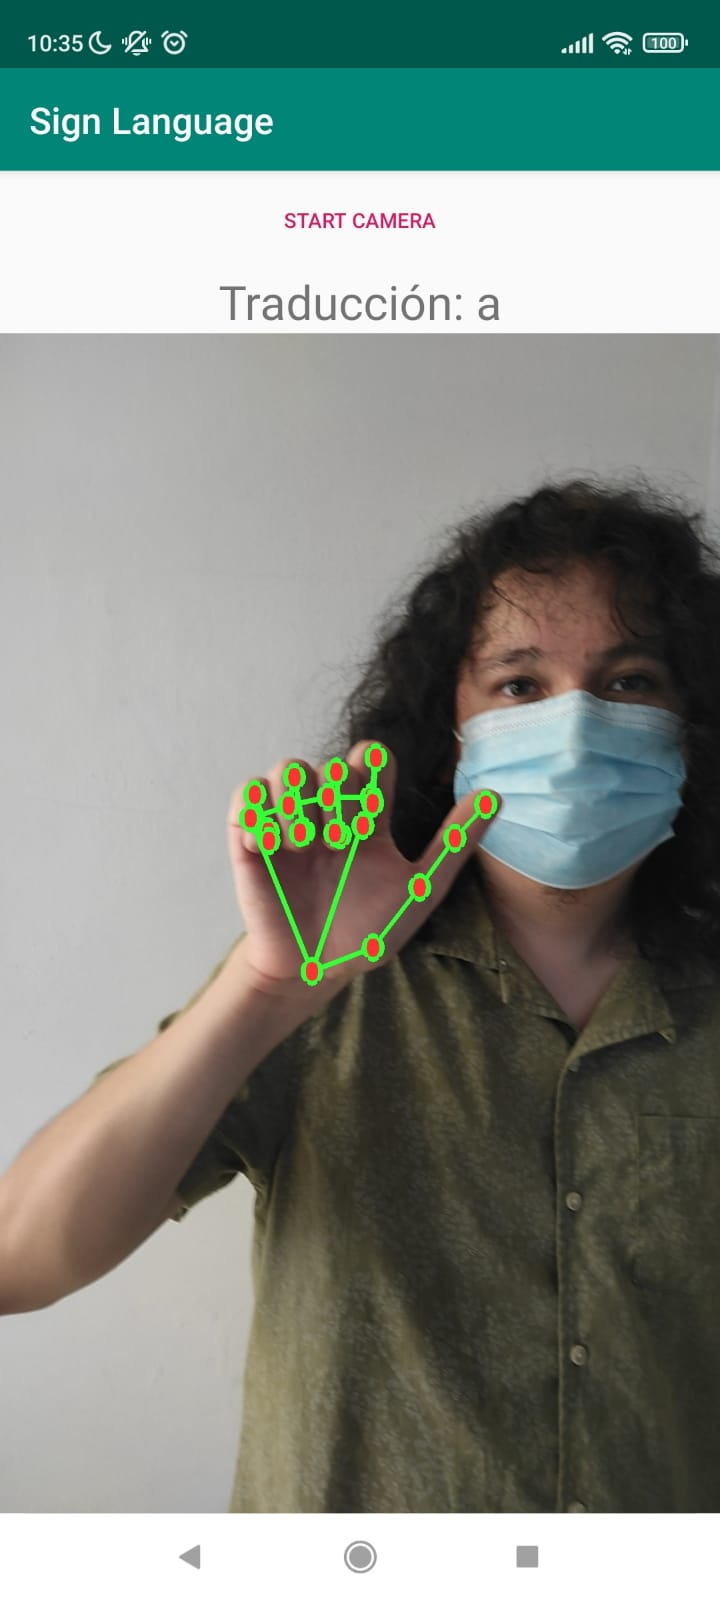
\includegraphics[width=0.16\textwidth]{2022_AplicacionLSM/figs/Muestra_compañeros1.jpeg}
    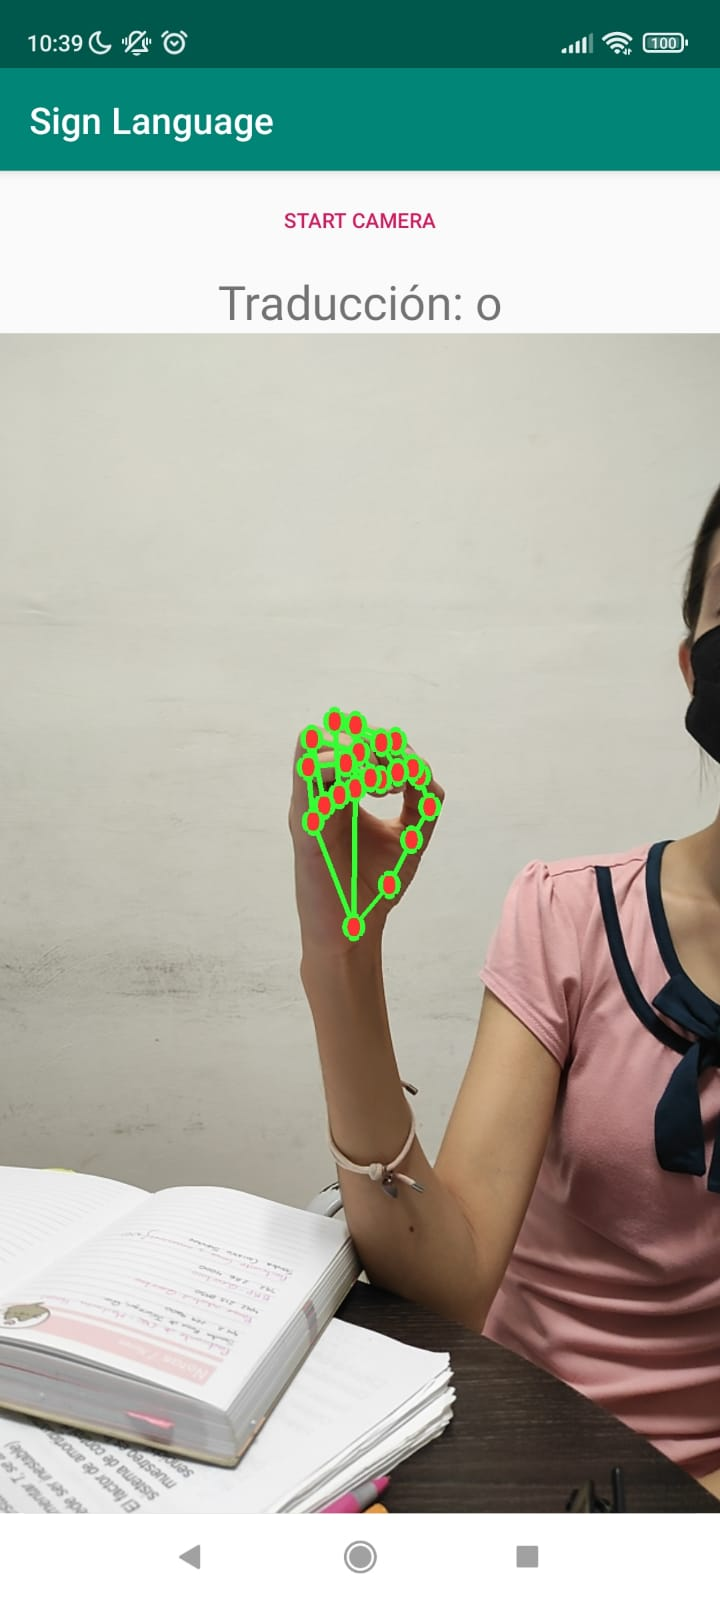
\includegraphics[width=0.16\textwidth]{2022_AplicacionLSM/figs/Muestra_compañeros2.jpeg}
  \end{tabular}
\end{center}

\end{frame}








\renewcommand{\EntradaBibtex}{AppComidaTamaulipeca_SistemasInteligentes_UPV_2023}


\begin{frame}{\citetitle{\EntradaBibtex} \footnotemark[1] (1)}
\begin{block}{Motivación} 
Desarrollar aplicación enfocada en la comida de una región para obtener información nutricional de la misma
\end{block} 
\begin{itemize}
\item Crear un modelo entrenado (usando TensorFlow) con imágenes de comida (gorditas, flautas, tamales, tortas y pozole)
\item Integar dicho modelo a una aplicación móvil (en Android) 
\item Al tomar una foto con la aplicación, se indique de que alimento se trata, además de su información nutrimental
\end{itemize}
\footnotetext[1]{\fullcite{\EntradaBibtex}}
\end{frame}

\begin{frame}{\citetitle{\EntradaBibtex} (2)}

\begin{center}
	\begin{tabular}{ccccc}
		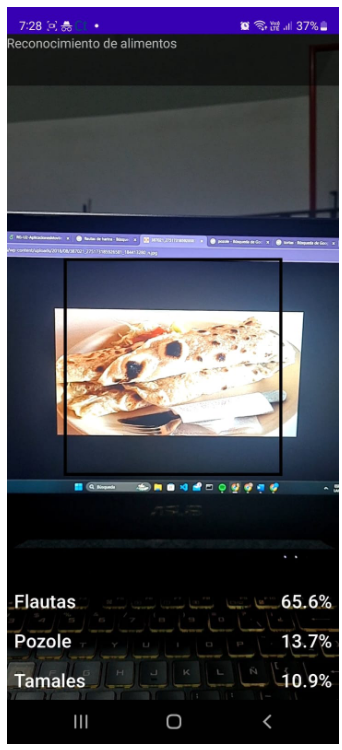
\includegraphics[width=0.18\linewidth,height=4.85cm]{2023_AppComidaTamaulipeca/figs/AppComida1.png} &
		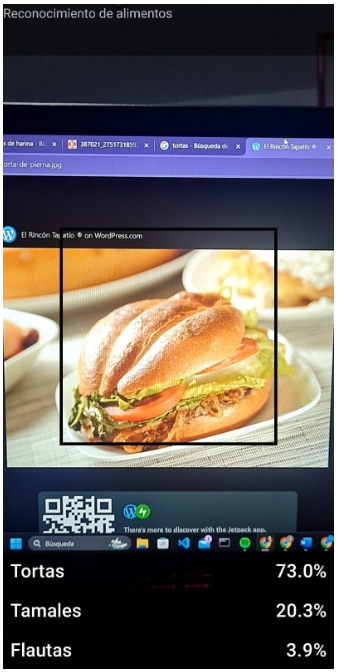
\includegraphics[width=0.18\linewidth,height=4.85cm]{2023_AppComidaTamaulipeca/figs/AppComida2.png} &
		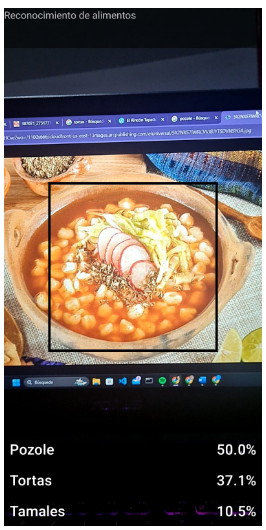
\includegraphics[width=0.18\linewidth,height=4.85cm]{2023_AppComidaTamaulipeca/figs/AppComida3.png} &
		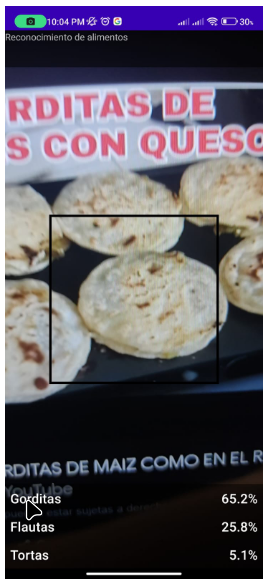
\includegraphics[width=0.18\linewidth,height=4.85cm]{2023_AppComidaTamaulipeca/figs/AppComida4.png} &
		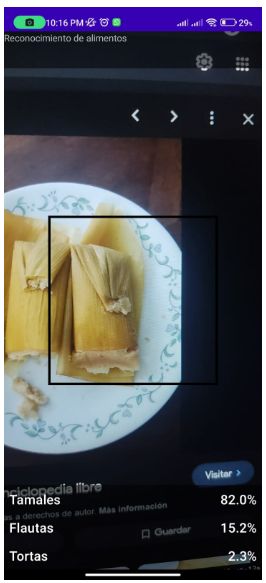
\includegraphics[width=0.18\linewidth,height=4.85cm]{2023_AppComidaTamaulipeca/figs/AppComida5.png}  \\
	\end{tabular}
\end{center}

\end{frame}

%




\renewcommand{\EntradaBibtex}{AppSegmentaCromosomas_SistemasInteligentes_UPV_2023}


\begin{frame}{\citetitle{\EntradaBibtex} \footnotemark[1] (1)}
\begin{block}{Motivación} 
Desarrollar aplicación móvil para que el Citogenetista localice los cromosomas en imágenes de estudios de citogenética y genere el Cariograma
\end{block} 
\begin{itemize}
\item El usario selecciona una carpeta con imágenes de cromosomas y la imagen de trabajo. 
\item Se incluyen funciones de paneo y acercamiento/alejamiento
\item Con el dedo hacer trazos sobre los cromosomas (definir el esqueleto). Personalizar el grosor y el color del trazo.
\item Una vez finalizado el trazo pregunta el número de cromosoma recién seleccionado (23 pares de cromosomas)
\item Al seleccionar todos los cromosomas, generar el Cariograma
\end{itemize}
\footnotetext[1]{\fullcite{\EntradaBibtex}}
\end{frame}

\begin{frame}{\citetitle{\EntradaBibtex} (2)}

\begin{center}
	\begin{tabular}{ccccc}
		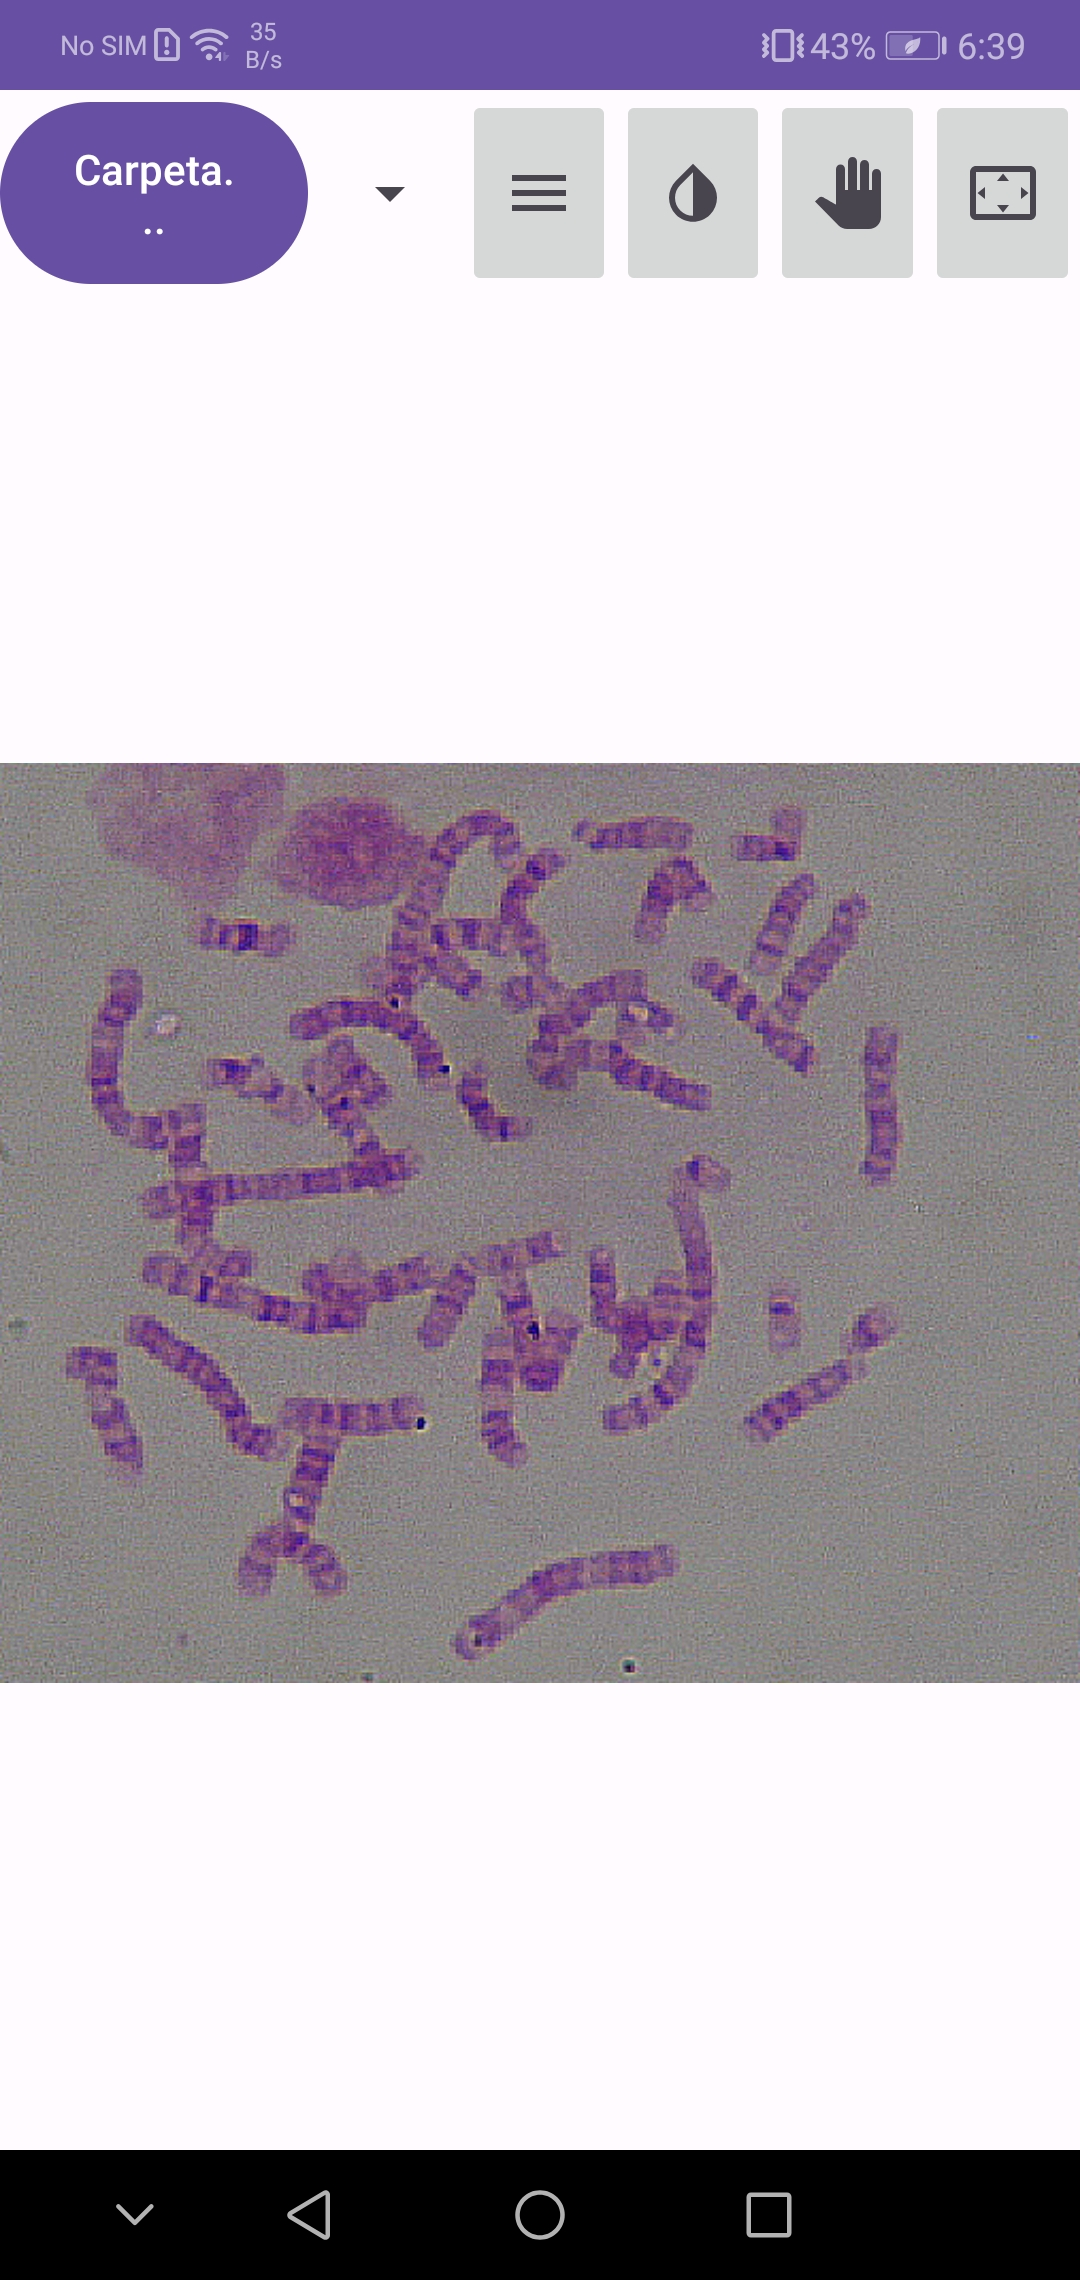
\includegraphics[width=0.18\linewidth,height=4.85cm]{2023_AppSegmentaCromosomas/figs/vistadeimagen.jpg}  &
		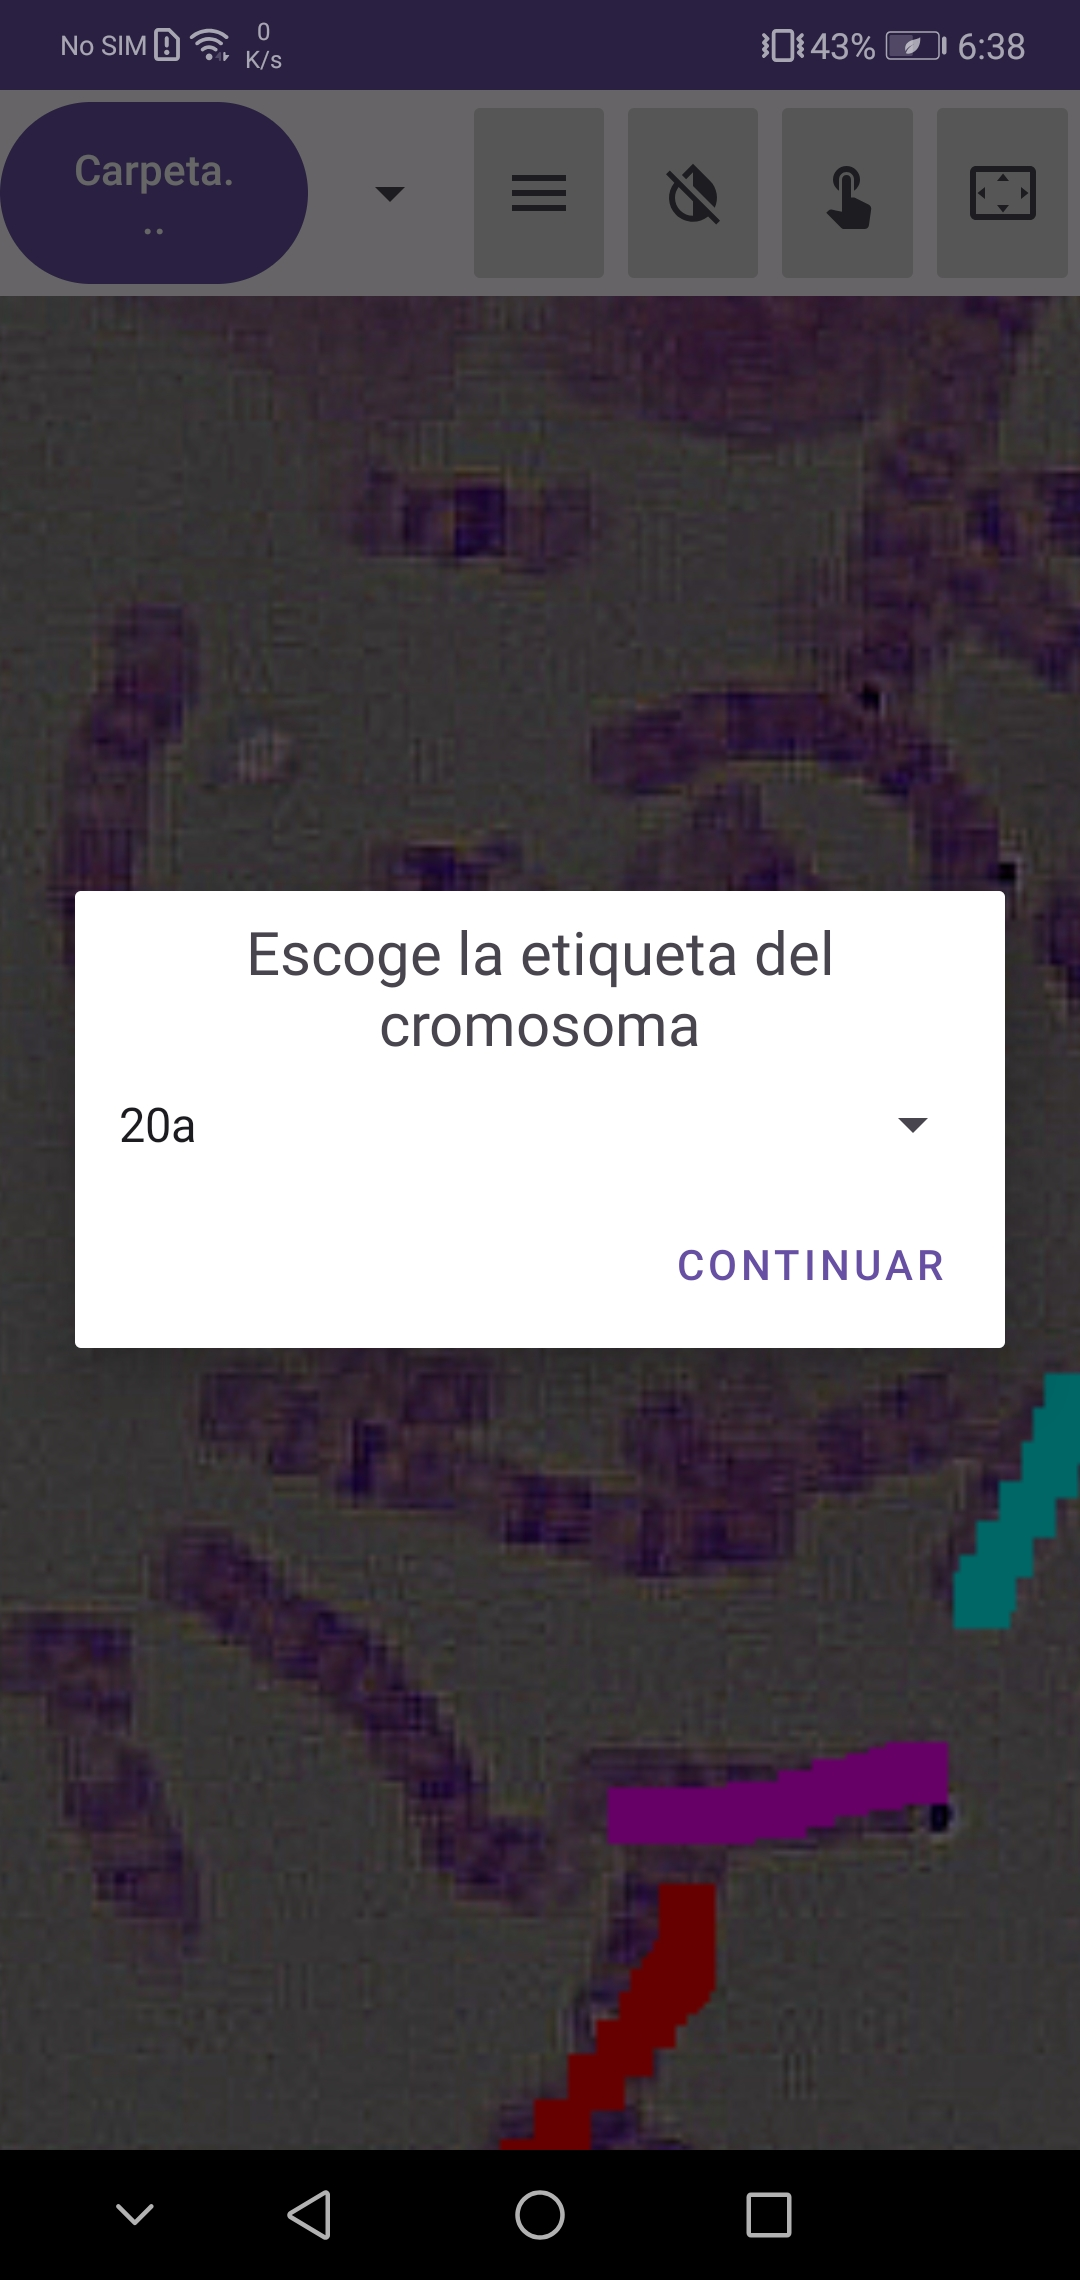
\includegraphics[width=0.18\linewidth,height=4.85cm]{2023_AppSegmentaCromosomas/figs/trazado.jpg} &		
		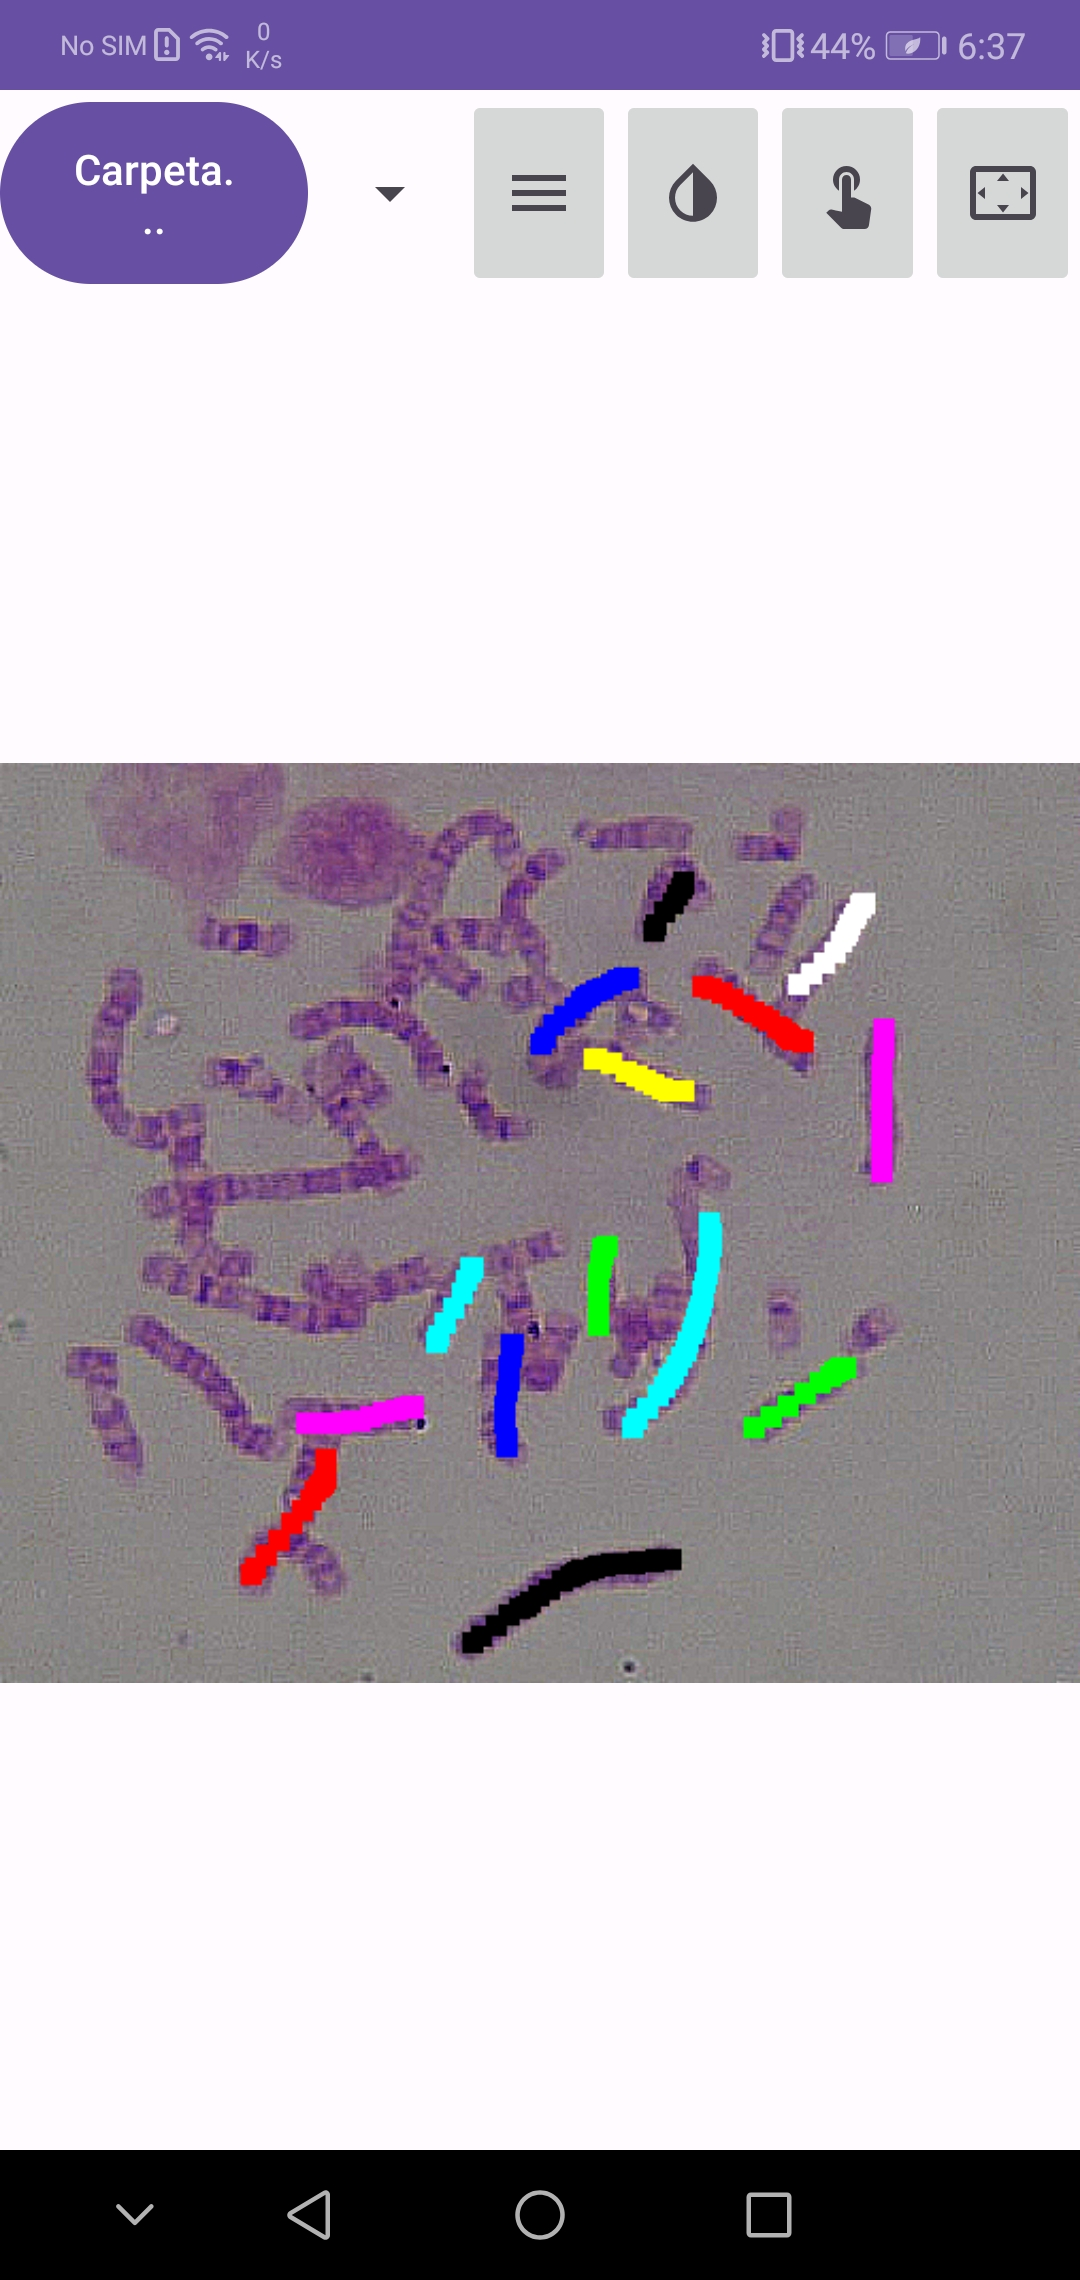
\includegraphics[width=0.18\linewidth,height=4.85cm]{2023_AppSegmentaCromosomas/figs/ediciondetrazo.jpg} &
		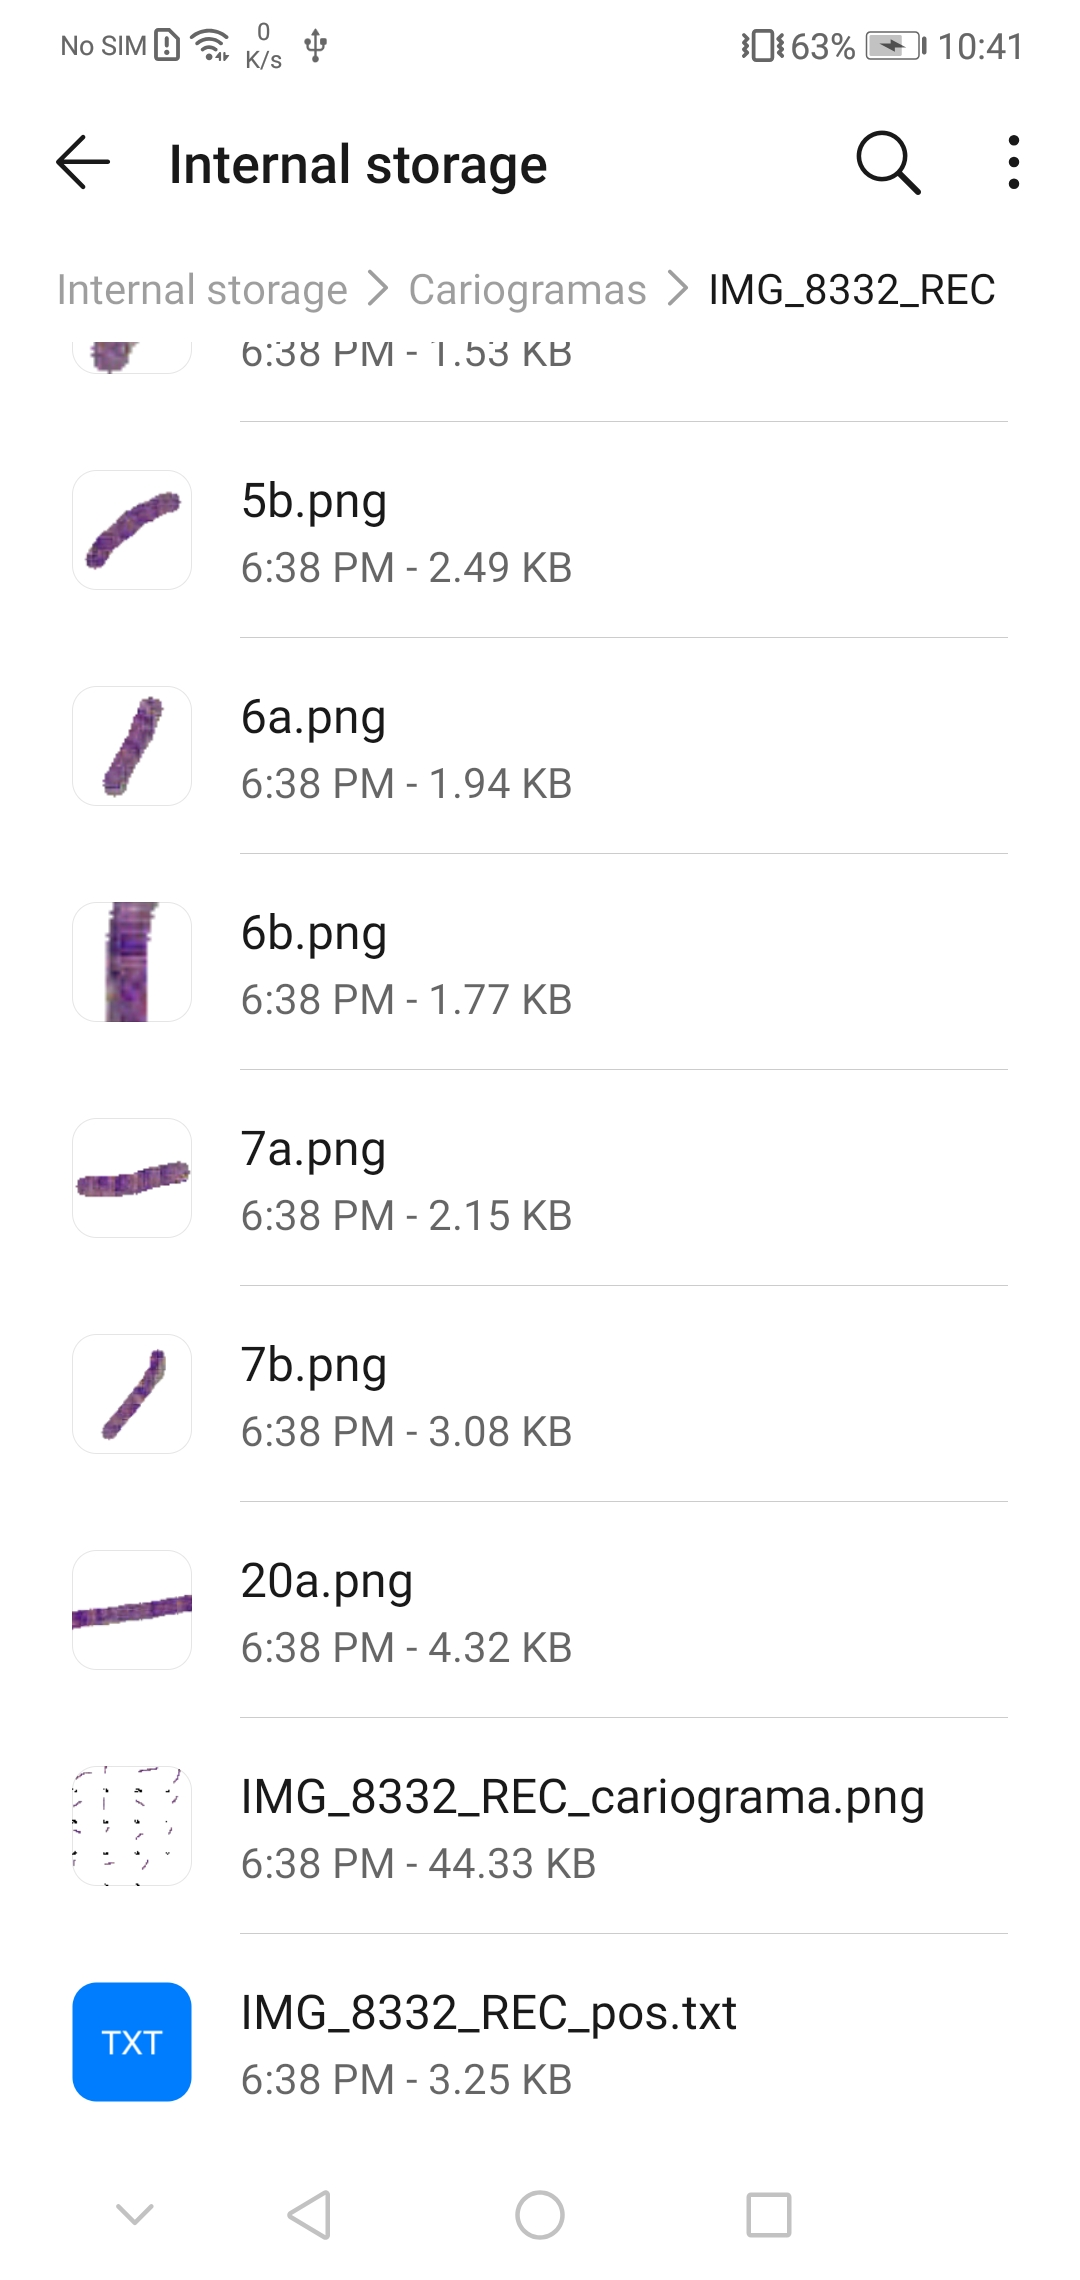
\includegraphics[width=0.18\linewidth,height=4.85cm]{2023_AppSegmentaCromosomas/figs/archivosdescargados.jpg} &
		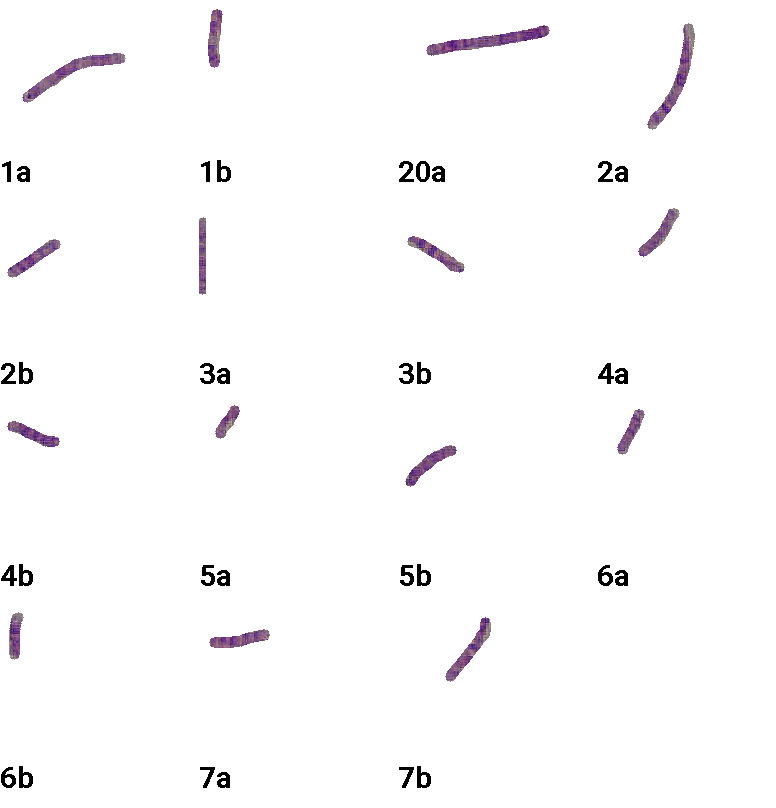
\includegraphics[width=0.18\linewidth,height=4.85cm]{2023_AppSegmentaCromosomas/figs/cariograma.png} \\
	\end{tabular}
\end{center}

\end{frame}


\begin{frame}{\citetitle{\EntradaBibtex} (3)}

\begin{center}
		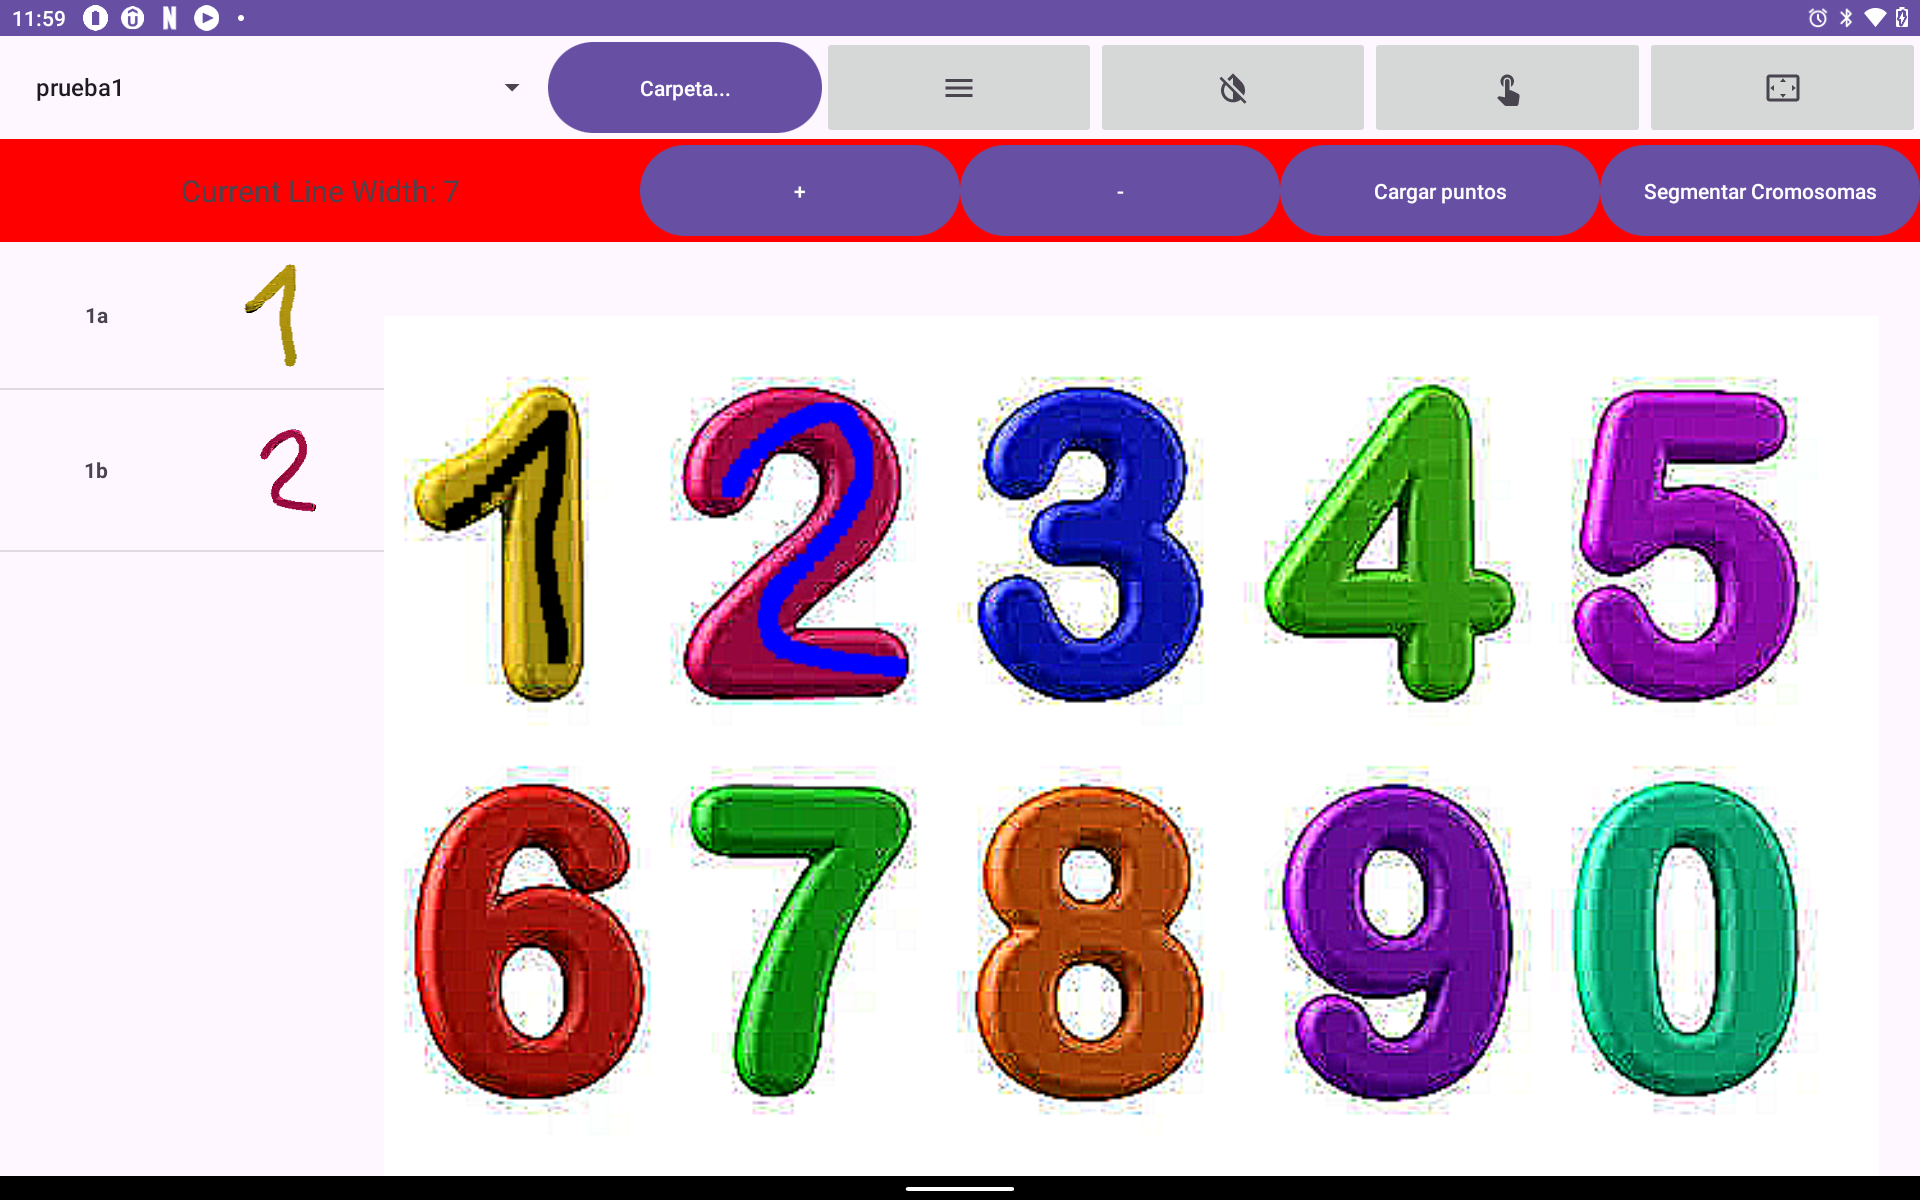
\includegraphics[width=0.70\linewidth]{2023_AppSegmentaCromosomas/figs/AppCromosomasTablet.png}  
\end{center}

\end{frame}


%




\renewcommand{\EntradaBibtex}{MarcoNuno_ReportePaseLista_2022}

\begin{frame}{\citetitle{\EntradaBibtex} \footnotemark[1] (1)}
\begin{block}{Motivación} 
Es necesario una herramienta que permita al profesor pasar asistencia de manera ágil y rápida. 
\begin{itemize}
\item El profesor debe ingresar los grupos a partir de archivos de texto
\item El profesor ingresa a pase de lista y selecciona uno de sus grupos
\item Puede seleccionar asistencia a todos o falta a todos para agilizar el proceso
\item La aplicacion genera un informe con las estadisticas de asistencias, faltas y retartdos
\item Originalmente la lista se manejaba por archivos de texto, despues se migró a una base de datos SQLite
\end{itemize}
\end{block} 
\footnotetext[1]{\fullcite{\EntradaBibtex}}
\end{frame}


\begin{frame}{\citetitle{\EntradaBibtex} (2)}
%\begin{block}{Pantallas Principales} 
\begin{center}
	\begin{tabular}{cccc}
		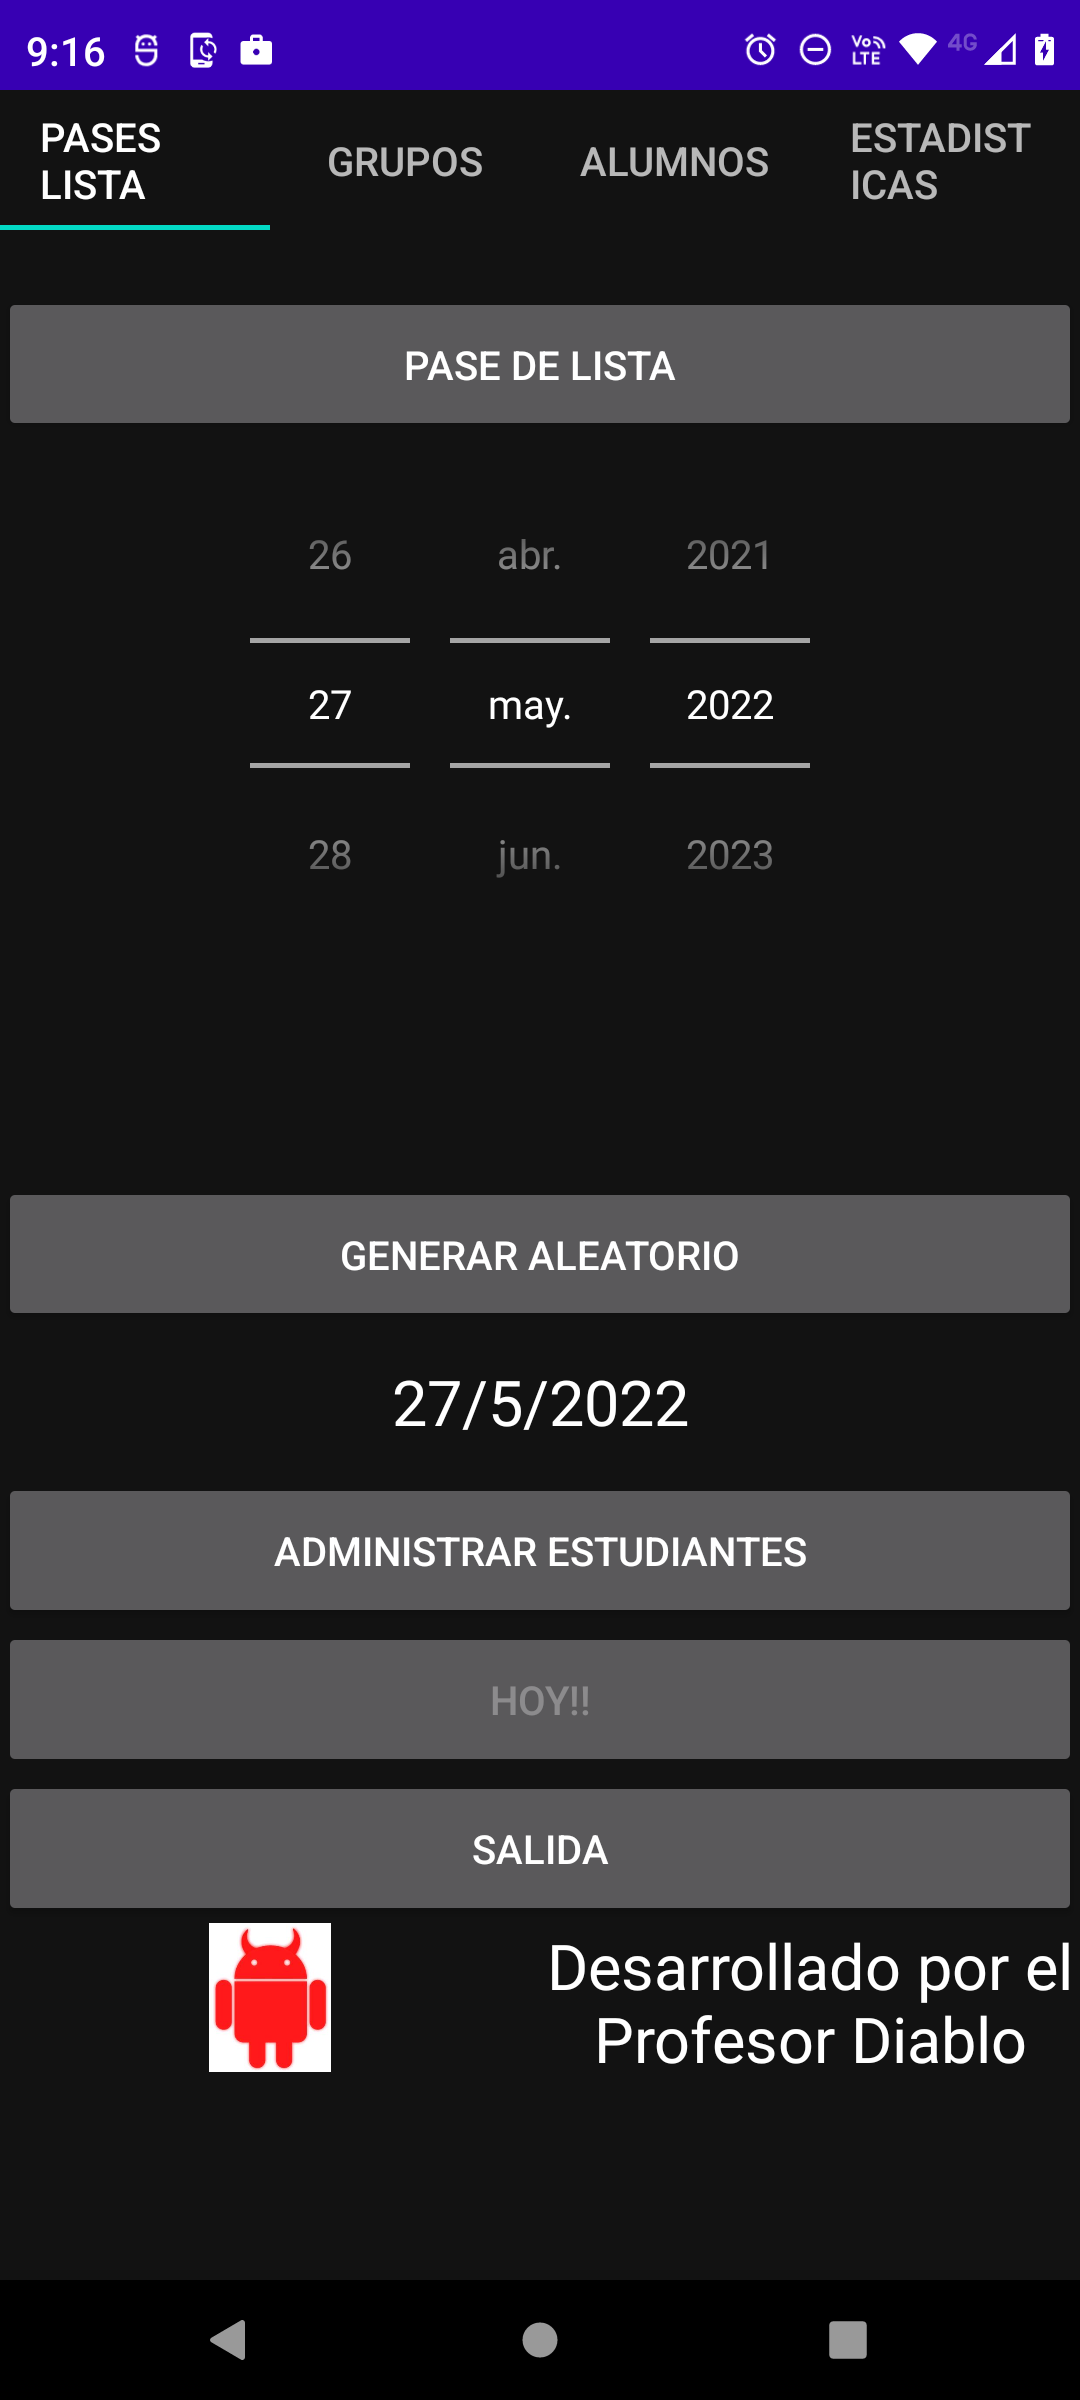
\includegraphics[width=0.20\linewidth]{2022_AppPaseLista/figs/PaseLista0.png} &
		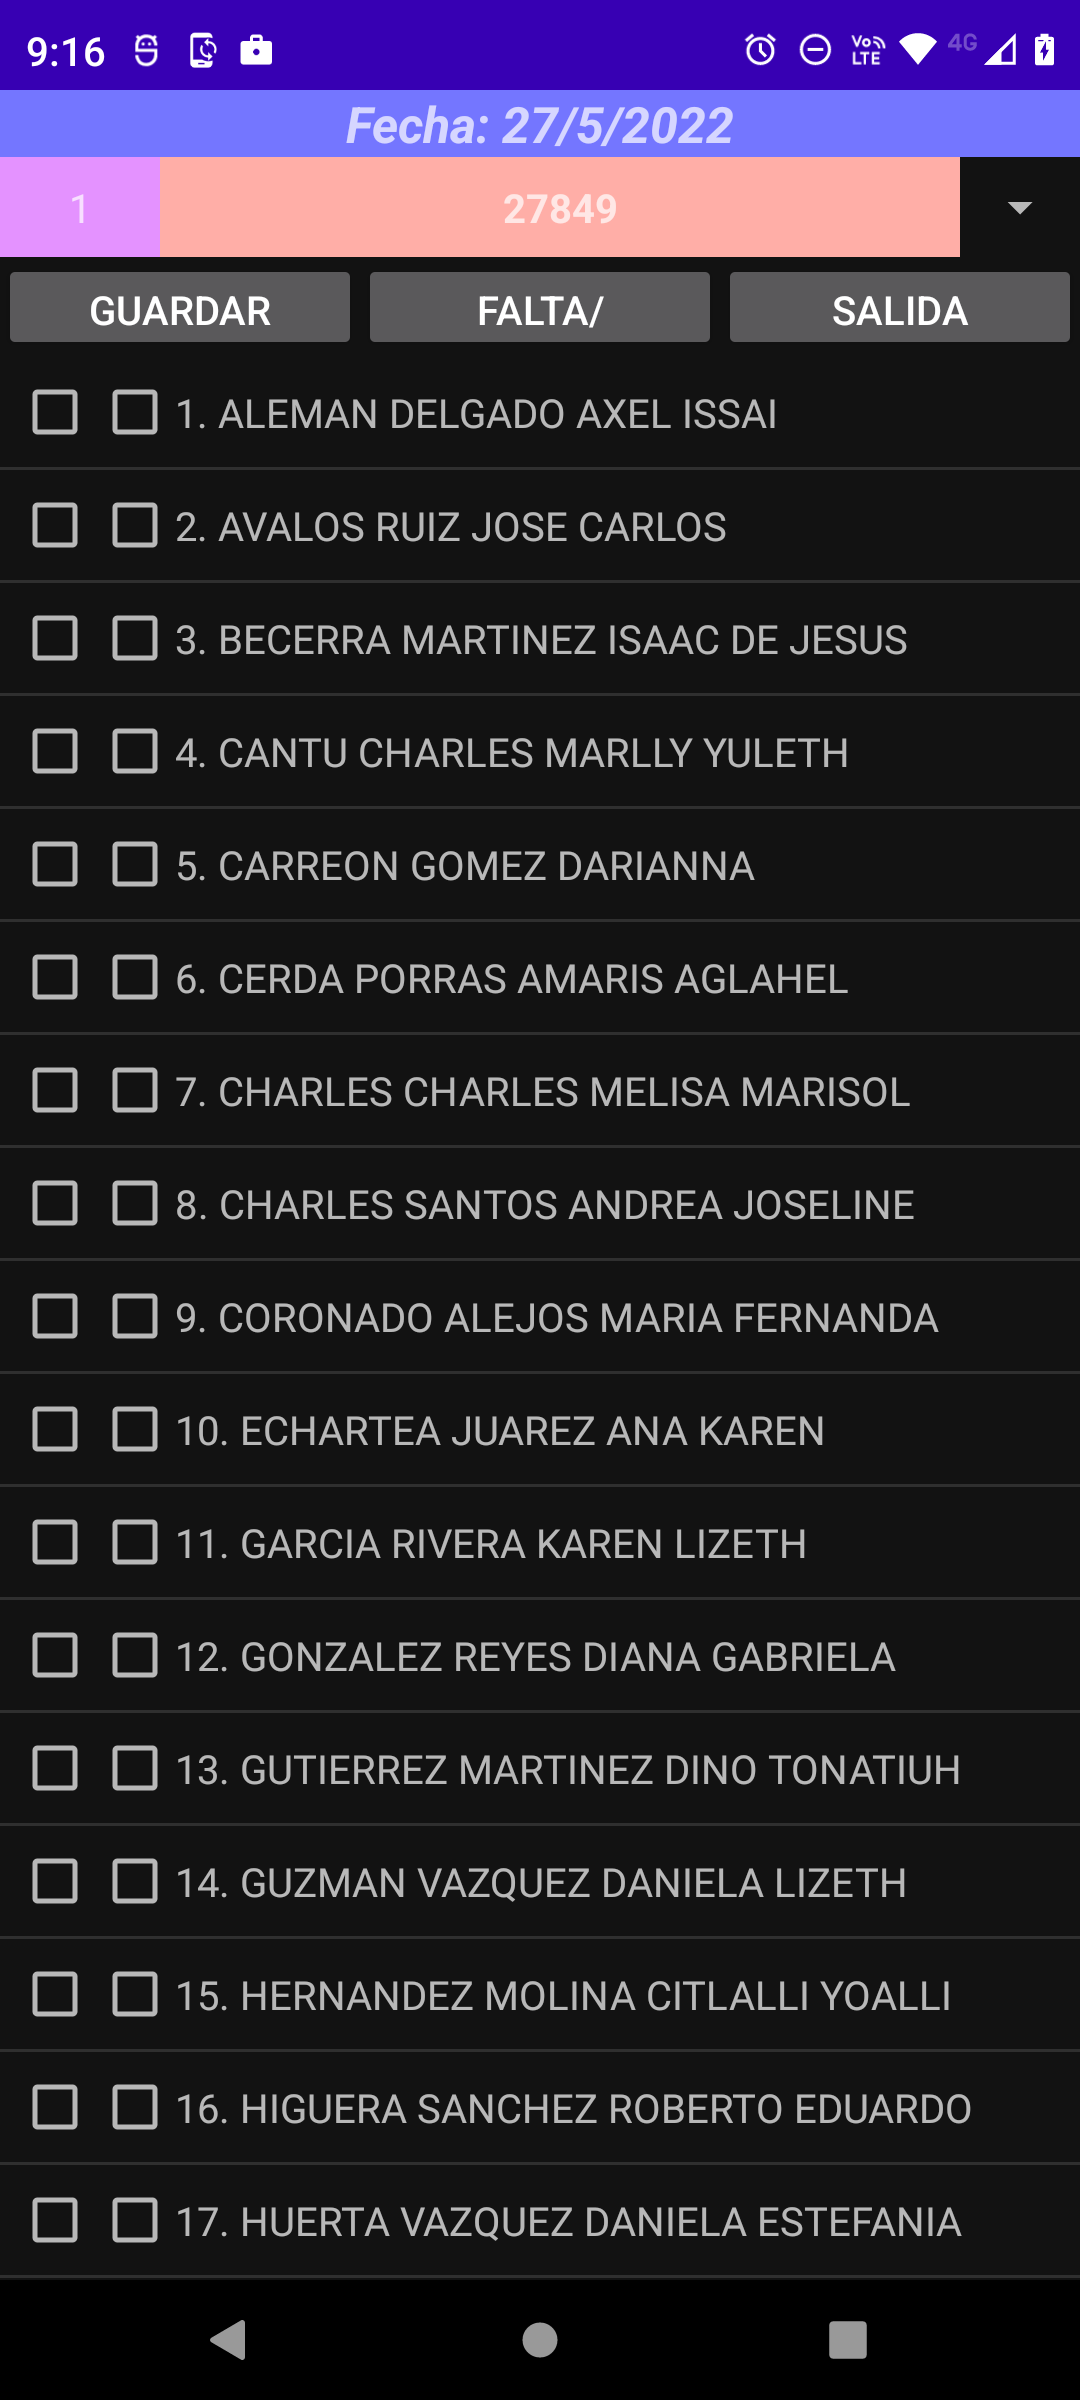
\includegraphics[width=0.20\linewidth]{2022_AppPaseLista/figs/PaseLista1.png} & 		 		
		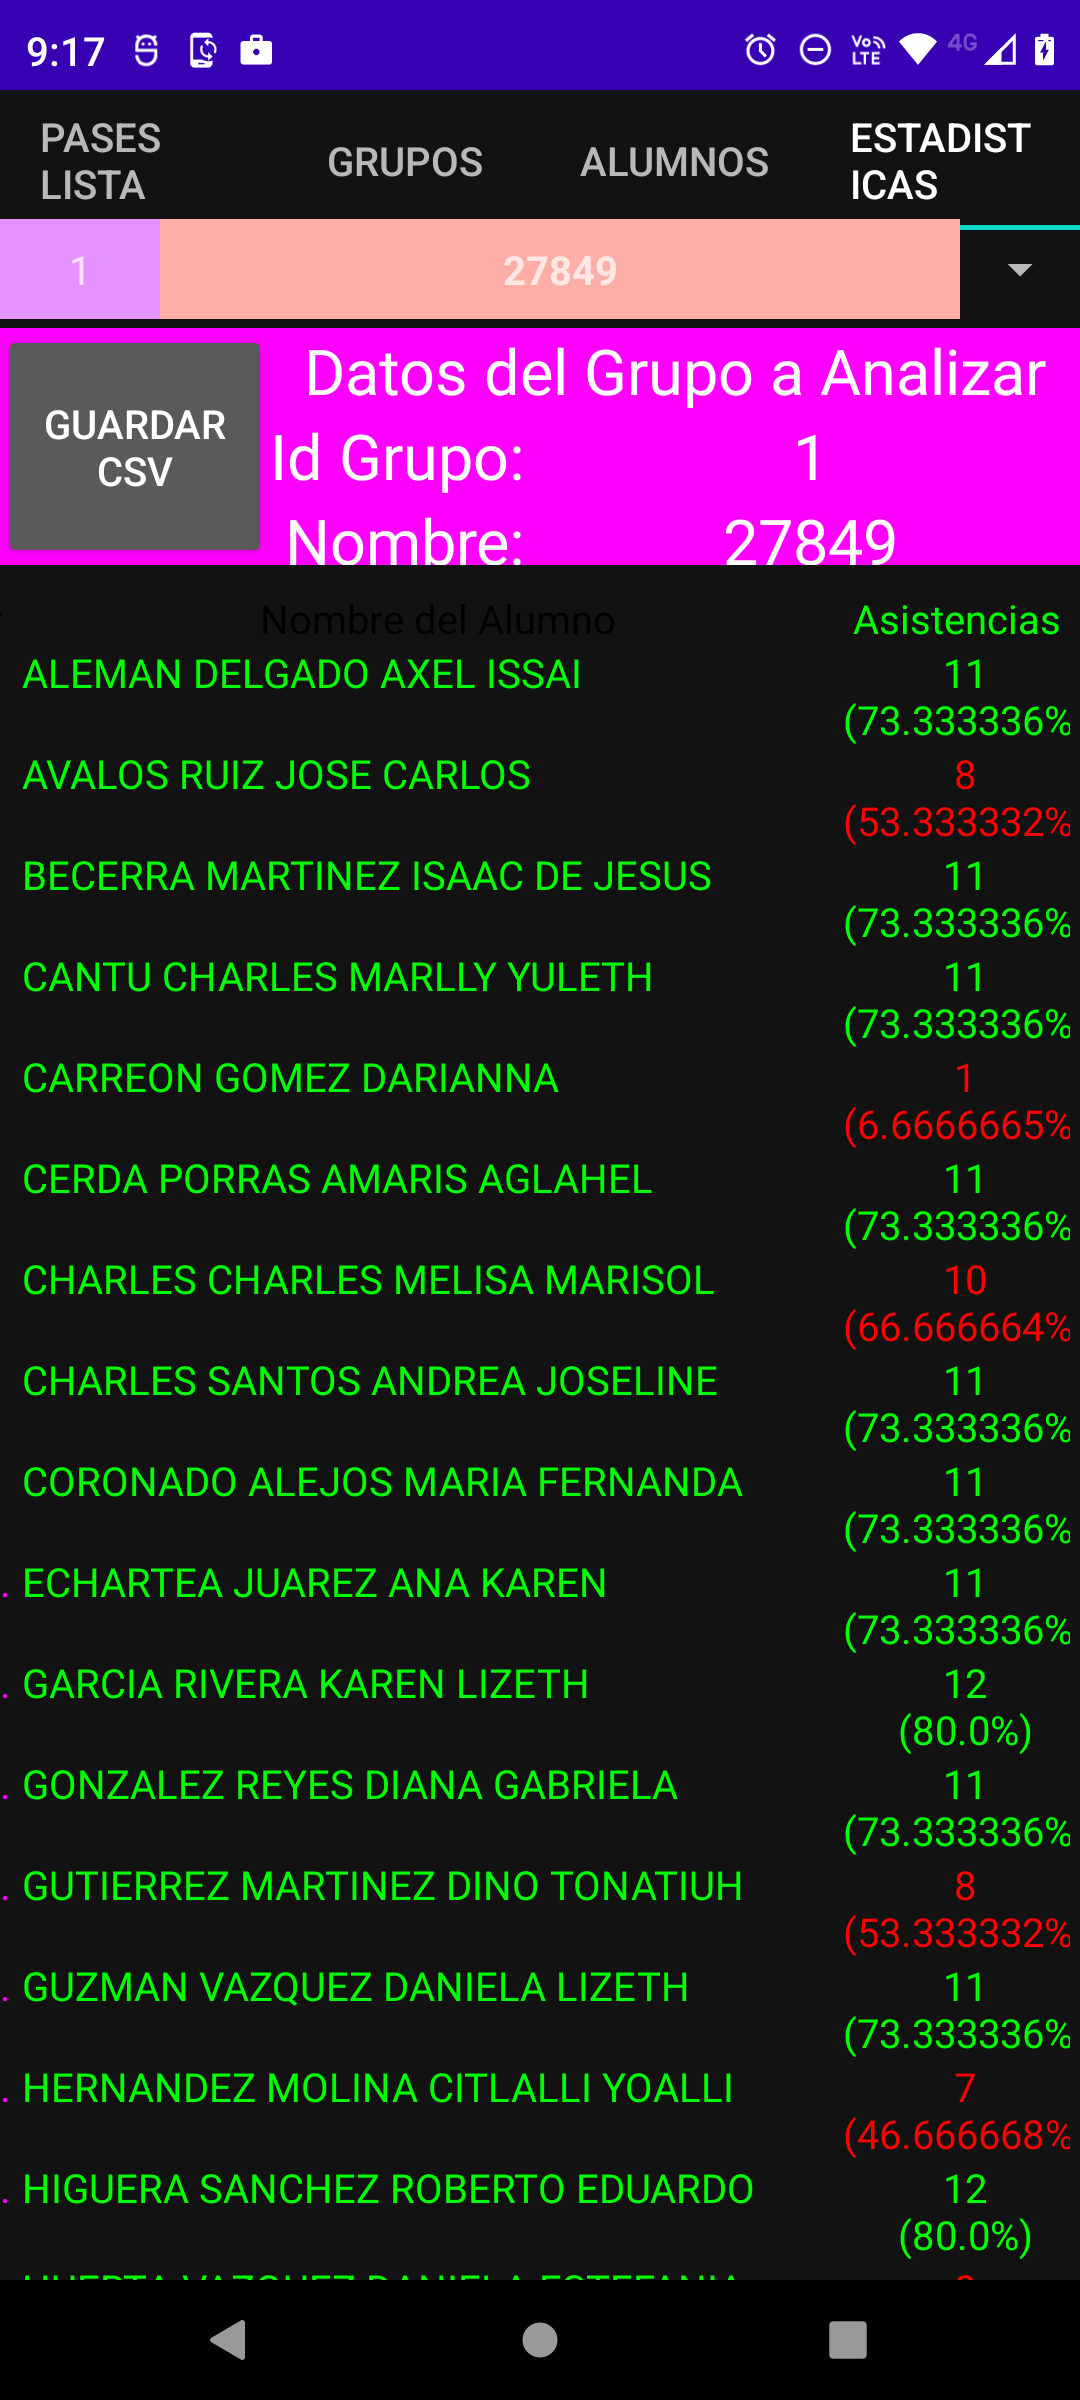
\includegraphics[width=0.20\linewidth]{2022_AppPaseLista/figs/PaseLista2.png} & 		
		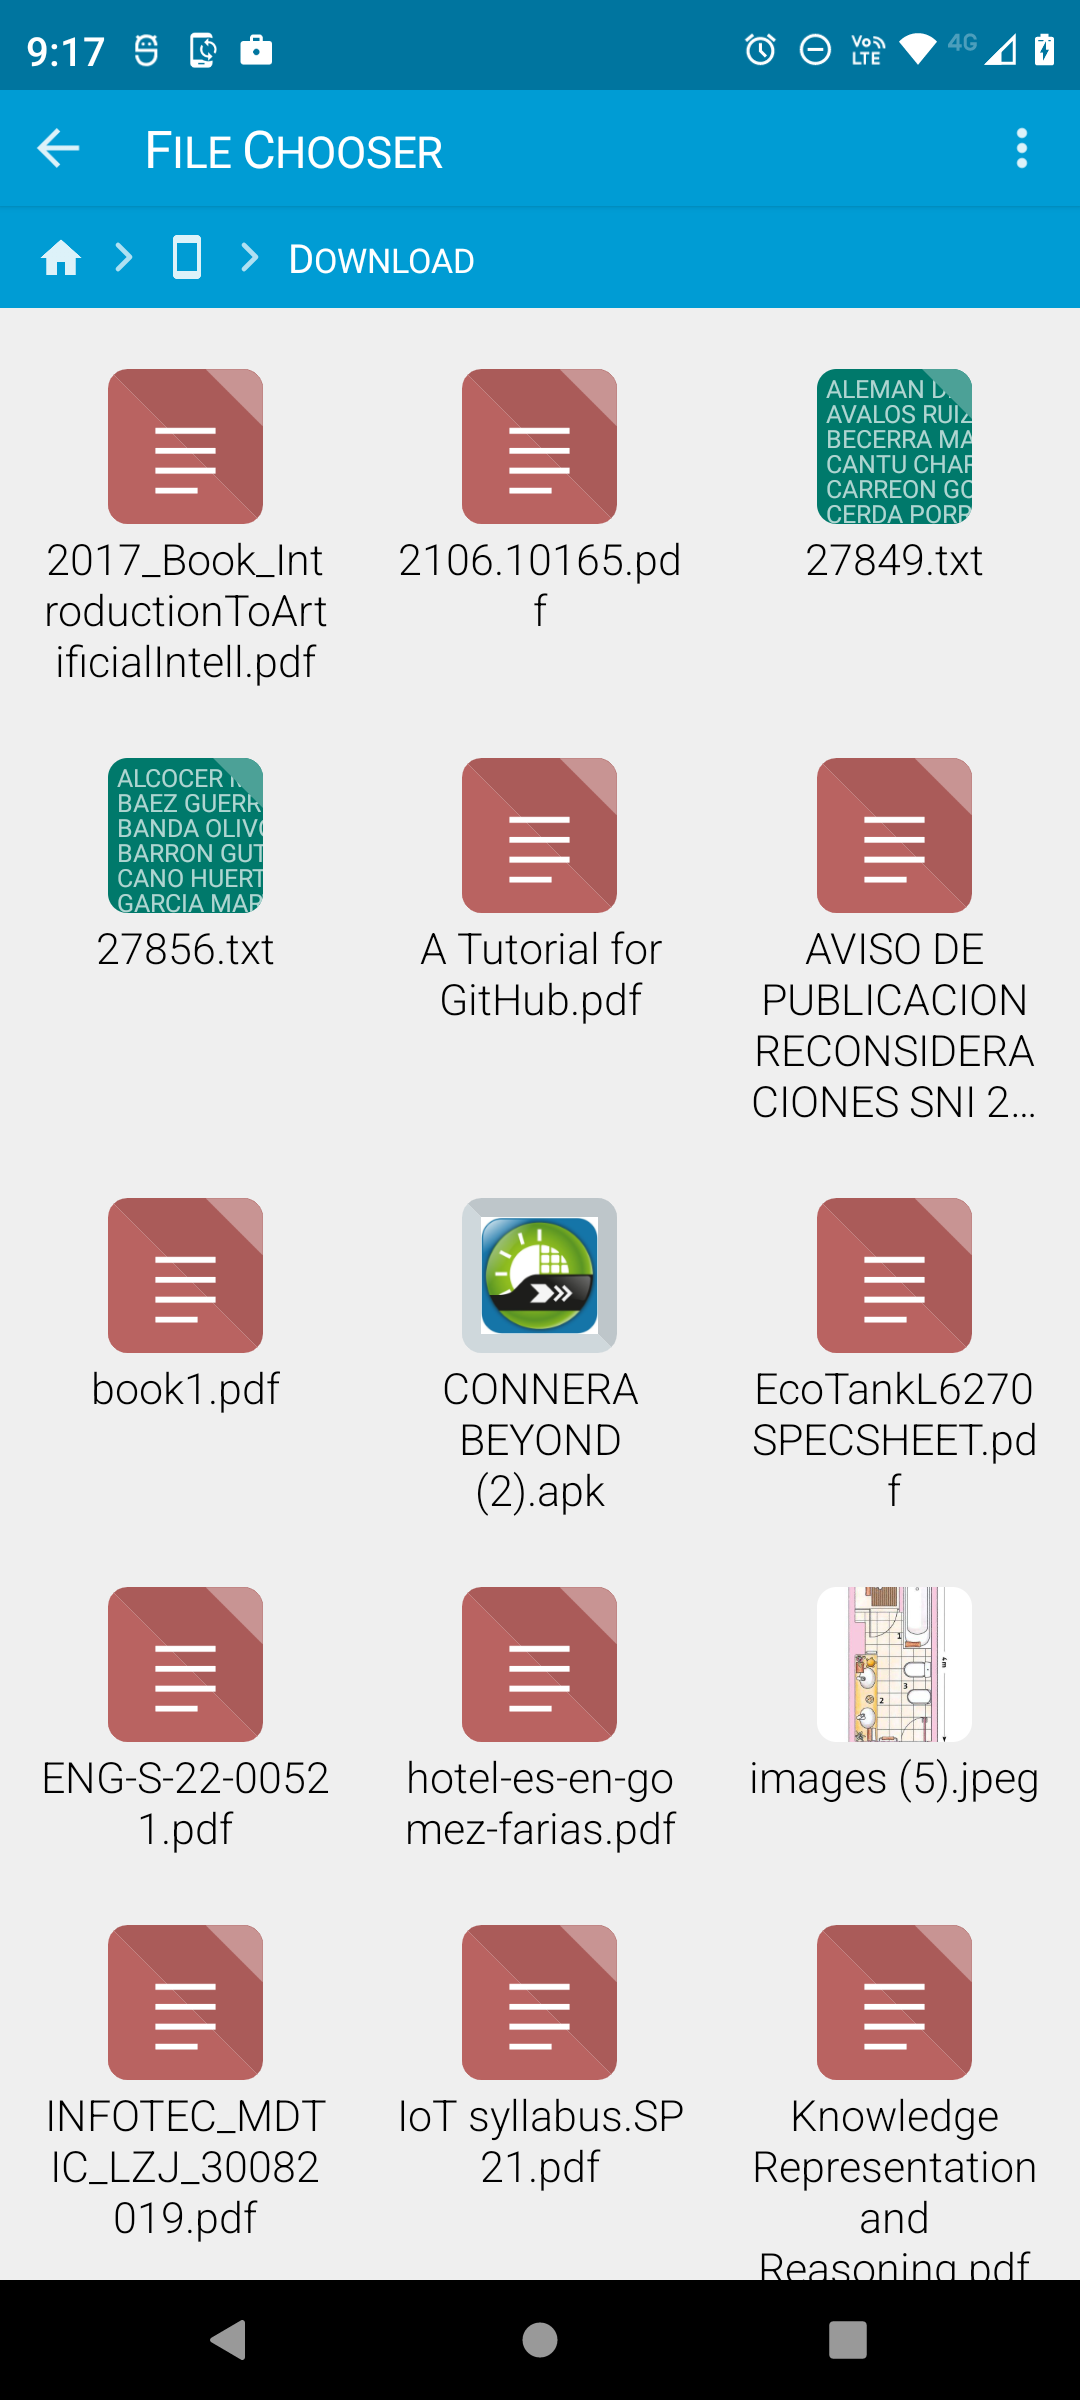
\includegraphics[width=0.20\linewidth]{2022_AppPaseLista/figs/PaseLista3.png} \\
	\end{tabular}
\end{center}
\end{frame}





\renewcommand{\EntradaBibtex}{PaseListasCodigoQRFaceDetection_SistemasInteligentes_UPV_2024}

\begin{frame}{\citetitle{\EntradaBibtex}$^*$ (1)}
\begin{block}{Motivación} 
Se requiere una herramienta que permita efectuar un pase de lista efectivo en grupos numerosos. 
\begin{itemize}
\item Se capturan fotografias de los asistentes del grupo, además de asignar a cada alumno de un código QR
\item Se emplea un modelo un módulo de Python denominado \textit{face-recognition} para entrena un modelo de aprendizaje profundo para reconocer los rostros de los asistentes a la clase
\item Se emplea una librería para detección de códigos QR
\item Se cruza la información de la identidad del estudiante con el código QR
\end{itemize}
\end{block} 
\footfullcite*{\EntradaBibtex}
\end{frame}


\begin{frame}{\citetitle{\EntradaBibtex} (2)}
%\begin{block}{Pantallas Principales} 

%\begin{columns}
% Column 1
%\column{.1\linewidth}
%\begin{center}
%\includegraphics[width=0.85\linewidth]{2024_DetectorMotos/figs/resultados1.png}
%\includegraphics[width=0.85\linewidth]{2024_DetectorMotos/figs/resultados2.png}
%\end{center}
%\column{.9\linewidth}
\begin{center}
	\begin{tabular}{ccc}
		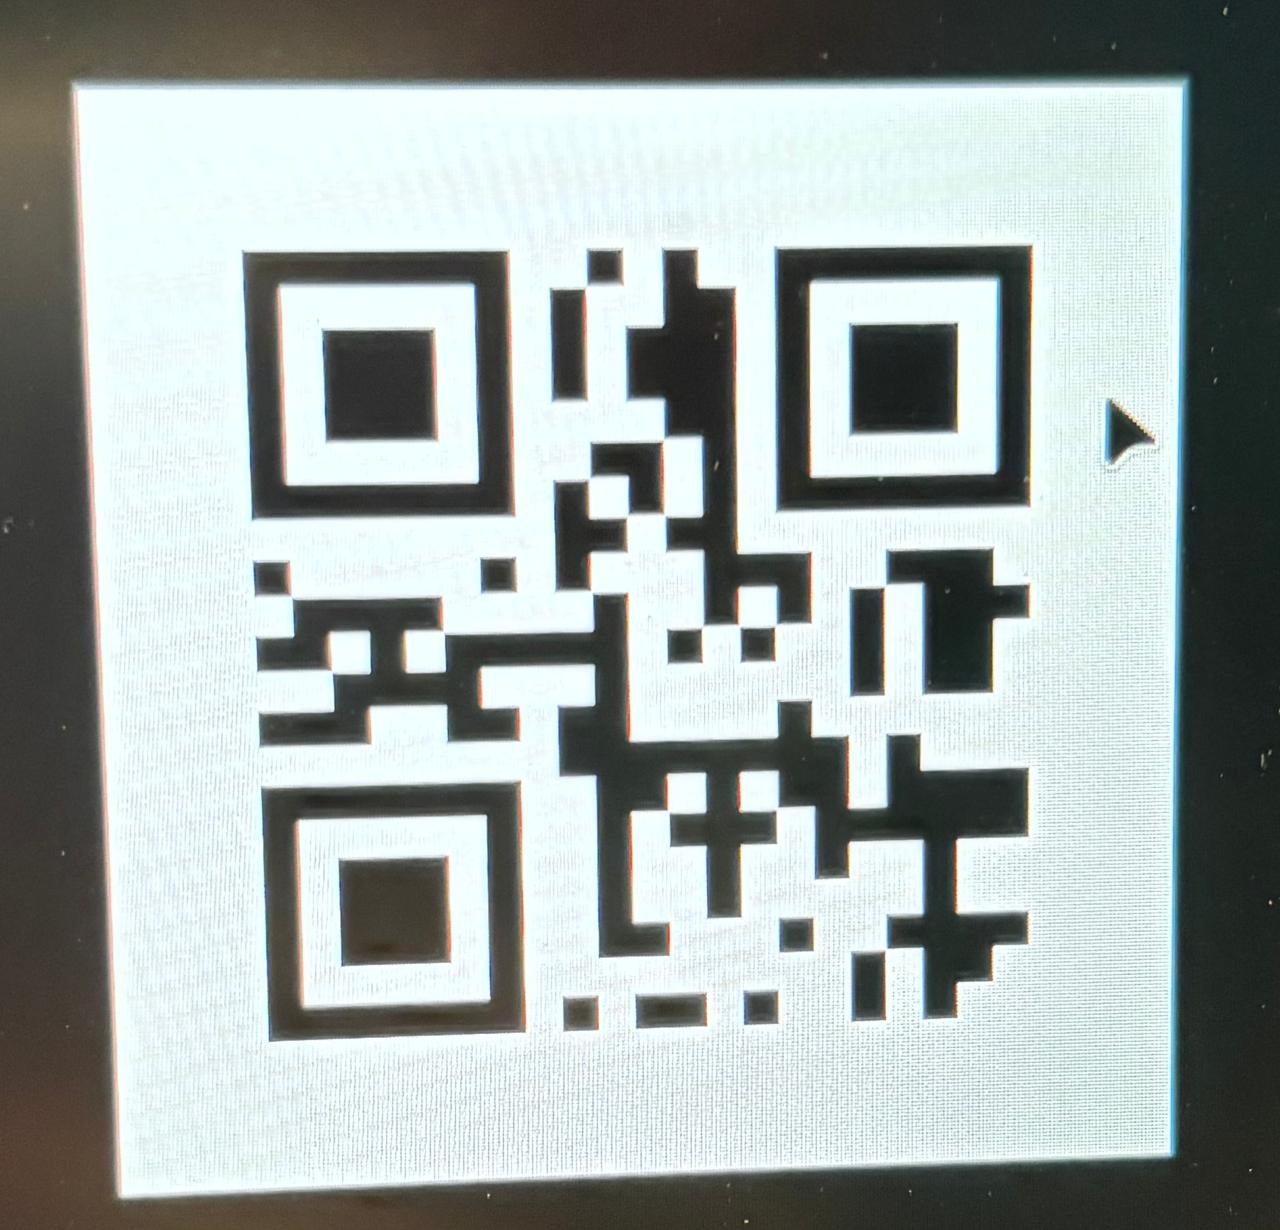
\includegraphics[width=0.20\linewidth]{2024_PaseDeListaCodigoQR/figs/2.jpg} &
		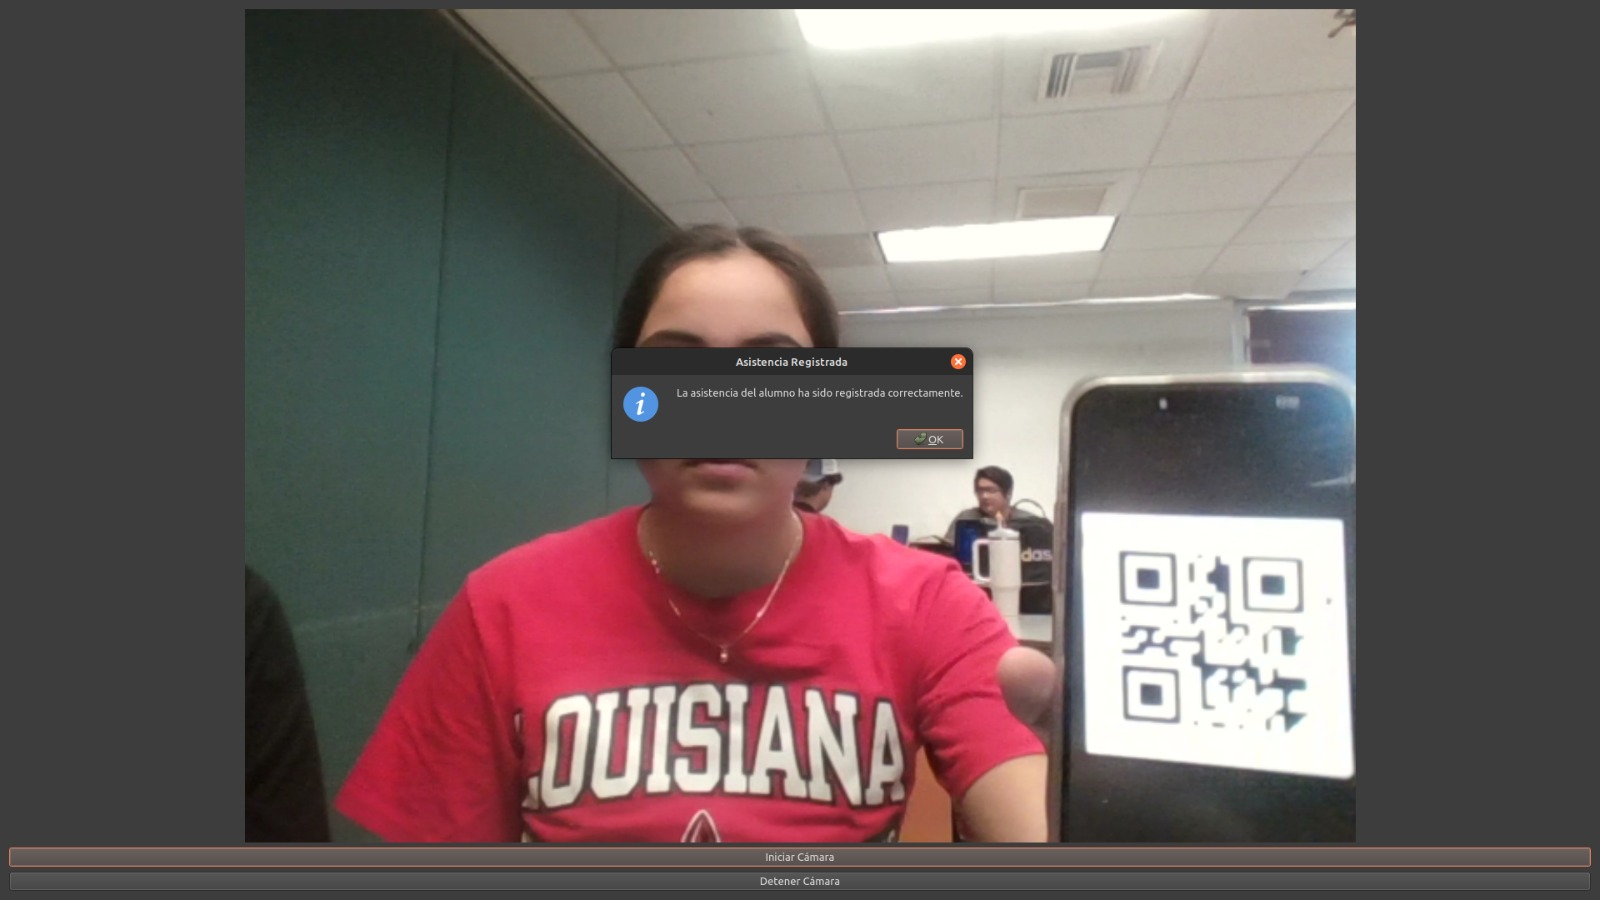
\includegraphics[width=0.38\linewidth]{2024_PaseDeListaCodigoQR/figs/3.jpg} &
 		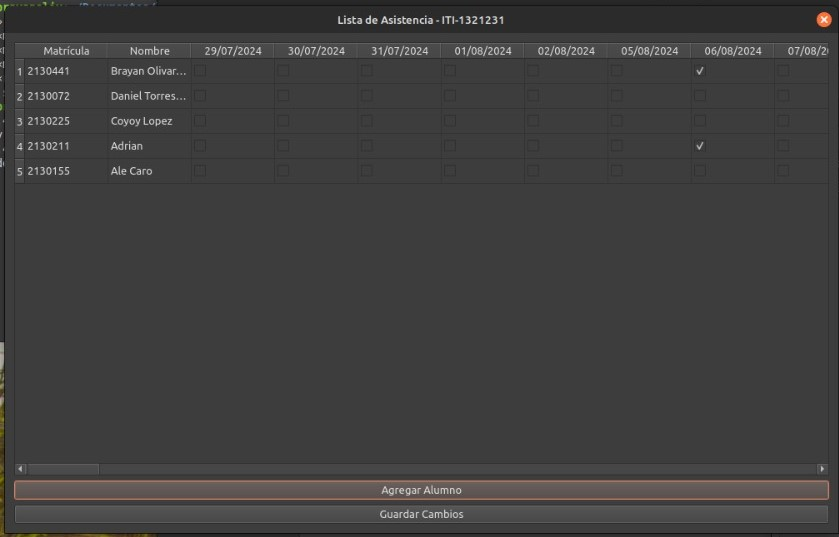
\includegraphics[width=0.38\linewidth]{2024_PaseDeListaCodigoQR/figs/4.jpg} \\
	\end{tabular}
\end{center}

%\end{columns}
\end{frame}

%/media/marco/Master/00_0A0RespadoLaptopHP_2024/Escritorio/00_DiapositivasProyectos/2024_PaseDeListaCodigoQR/figs/2.jpg
%/media/marco/Master/00_0A0RespadoLaptopHP_2024/Escritorio/00_DiapositivasProyectos/2024_PaseDeListaCodigoQR/figs/3.jpg
%/media/marco/Master/00_0A0RespadoLaptopHP_2024/Escritorio/00_DiapositivasProyectos/2024_PaseDeListaCodigoQR/figs/4.jpg




\subsection{Reconocimiento de partes del cuerpo}

\renewcommand{\Folder}{2025_SkinReplacement}
\renewcommand{\EntradaBibtex}{2025_SkinReplacement}

\begin{frame}{\citetitle{\EntradaBibtex} \footnotemark[1] (1)}

\begin{columns}
	\begin{column}{0.58\textwidth}
		\begin{itemize}
			\item Se desarrolló una aplicación móvil para Android que utiliza librerías de visión por computadora (OpenCV) para modificar el color de la piel en tiempo real.
			\item La aplicación detecta las áreas de piel mediante la combinación de los espacios de color HSV y YCrCb, permitiendo su aclarado u oscurecimiento con un control deslizante, además de alternar entre cámaras y capturar fotos con el efecto aplicado.
		\end{itemize}
	\end{column}
	\begin{column}{0.2\textwidth}
		 \begin{center}
		     \includegraphics[width=0.98\textwidth]{\Folder/figs/ejemplo_efecto_aplicado}
		 \end{center}
	\end{column}
	\begin{column}{0.2\textwidth}
		 \begin{center}
		     \includegraphics[width=0.98\textwidth]{\Folder/figs/ejemplo_mascara_piel}
		 \end{center}

	%\end{column}
	%\begin{column}{0.22\textwidth}  
		%\begin{center}
		 %\includegraphics[width=0.98\textwidth]{\Folder/figs/cuadroG}
		 %\end{center}
	\end{column}
\end{columns}
%\end{block} 
\footnotetext[1]{\fullcite{\EntradaBibtex}}
\end{frame}


\begin{frame}{\citetitle{\EntradaBibtex} \footnotemark[1] (2)}
%\begin{block}{Brazo Robótico \footnotemark} 
\begin{columns}
	\begin{column}{0.68\textwidth}
		\begin{itemize}
			\item Se logró implementar con éxito un algoritmo de detección de piel robusto, combinando los espacios de color HSV y YCrCb, con algunas limitaciones.  
            \item Las pruebas en tiempo real mostraron que el método es efectivo para identificar las áreas de piel en los fotogramas de la cámara, incluso bajo diferentes condiciones de iluminación. 
            \item Esto permitió generar una máscara binaria precisa que sirve como base para la aplicación del efecto.
		\end{itemize}
	\end{column}
	\begin{column}{0.3\textwidth}
		 \begin{center}
		     \includegraphics[width=0.98\textwidth]{\Folder/figs/dos_sujetos}
		 \end{center}
	\end{column}
	\begin{column}{0.02\textwidth}
		 \begin{center}
%		     \includegraphics[width=0.98\textwidth]{\Folder/figs/shownMunicipalityDetails}
		 \end{center}

	%\end{column}
	%\begin{column}{0.22\textwidth}  
		%\begin{center}
		 %\includegraphics[width=0.98\textwidth]{\Folder/figs/cuadroG}
		 %\end{center}
	\end{column}
\end{columns}
%\end{block} 
%\footnotetext[1]{\fullcite{\EntradaBibtex}}
\end{frame}



\renewcommand{\EntradaBibtex}{CurlBiceps_UPV_2024}

\begin{frame}{\citetitle{\EntradaBibtex}$^*$ (1)}
\begin{block}{Motivación} 
El curl de bı́ceps es un ejercicio que se centra en fortalecer y desarrollar los músculos del bíceps braquial, contribuyendo a la fuerza y definición de los brazos
\begin{itemize}
\item Se implementó una aplicación móvil
\begin{itemize}
\item Permite al usuario llevar el conteo de las repeticiones que deben ser de frente y simulateneas
\item Debe ubicar el dispositivo a una distancia de 80 cm. 
\item Si se levanta las pesas de forma asimétrica, el conteo no se modifica.
\end{itemize}
\end{itemize}
\end{block} 
\begin{center}
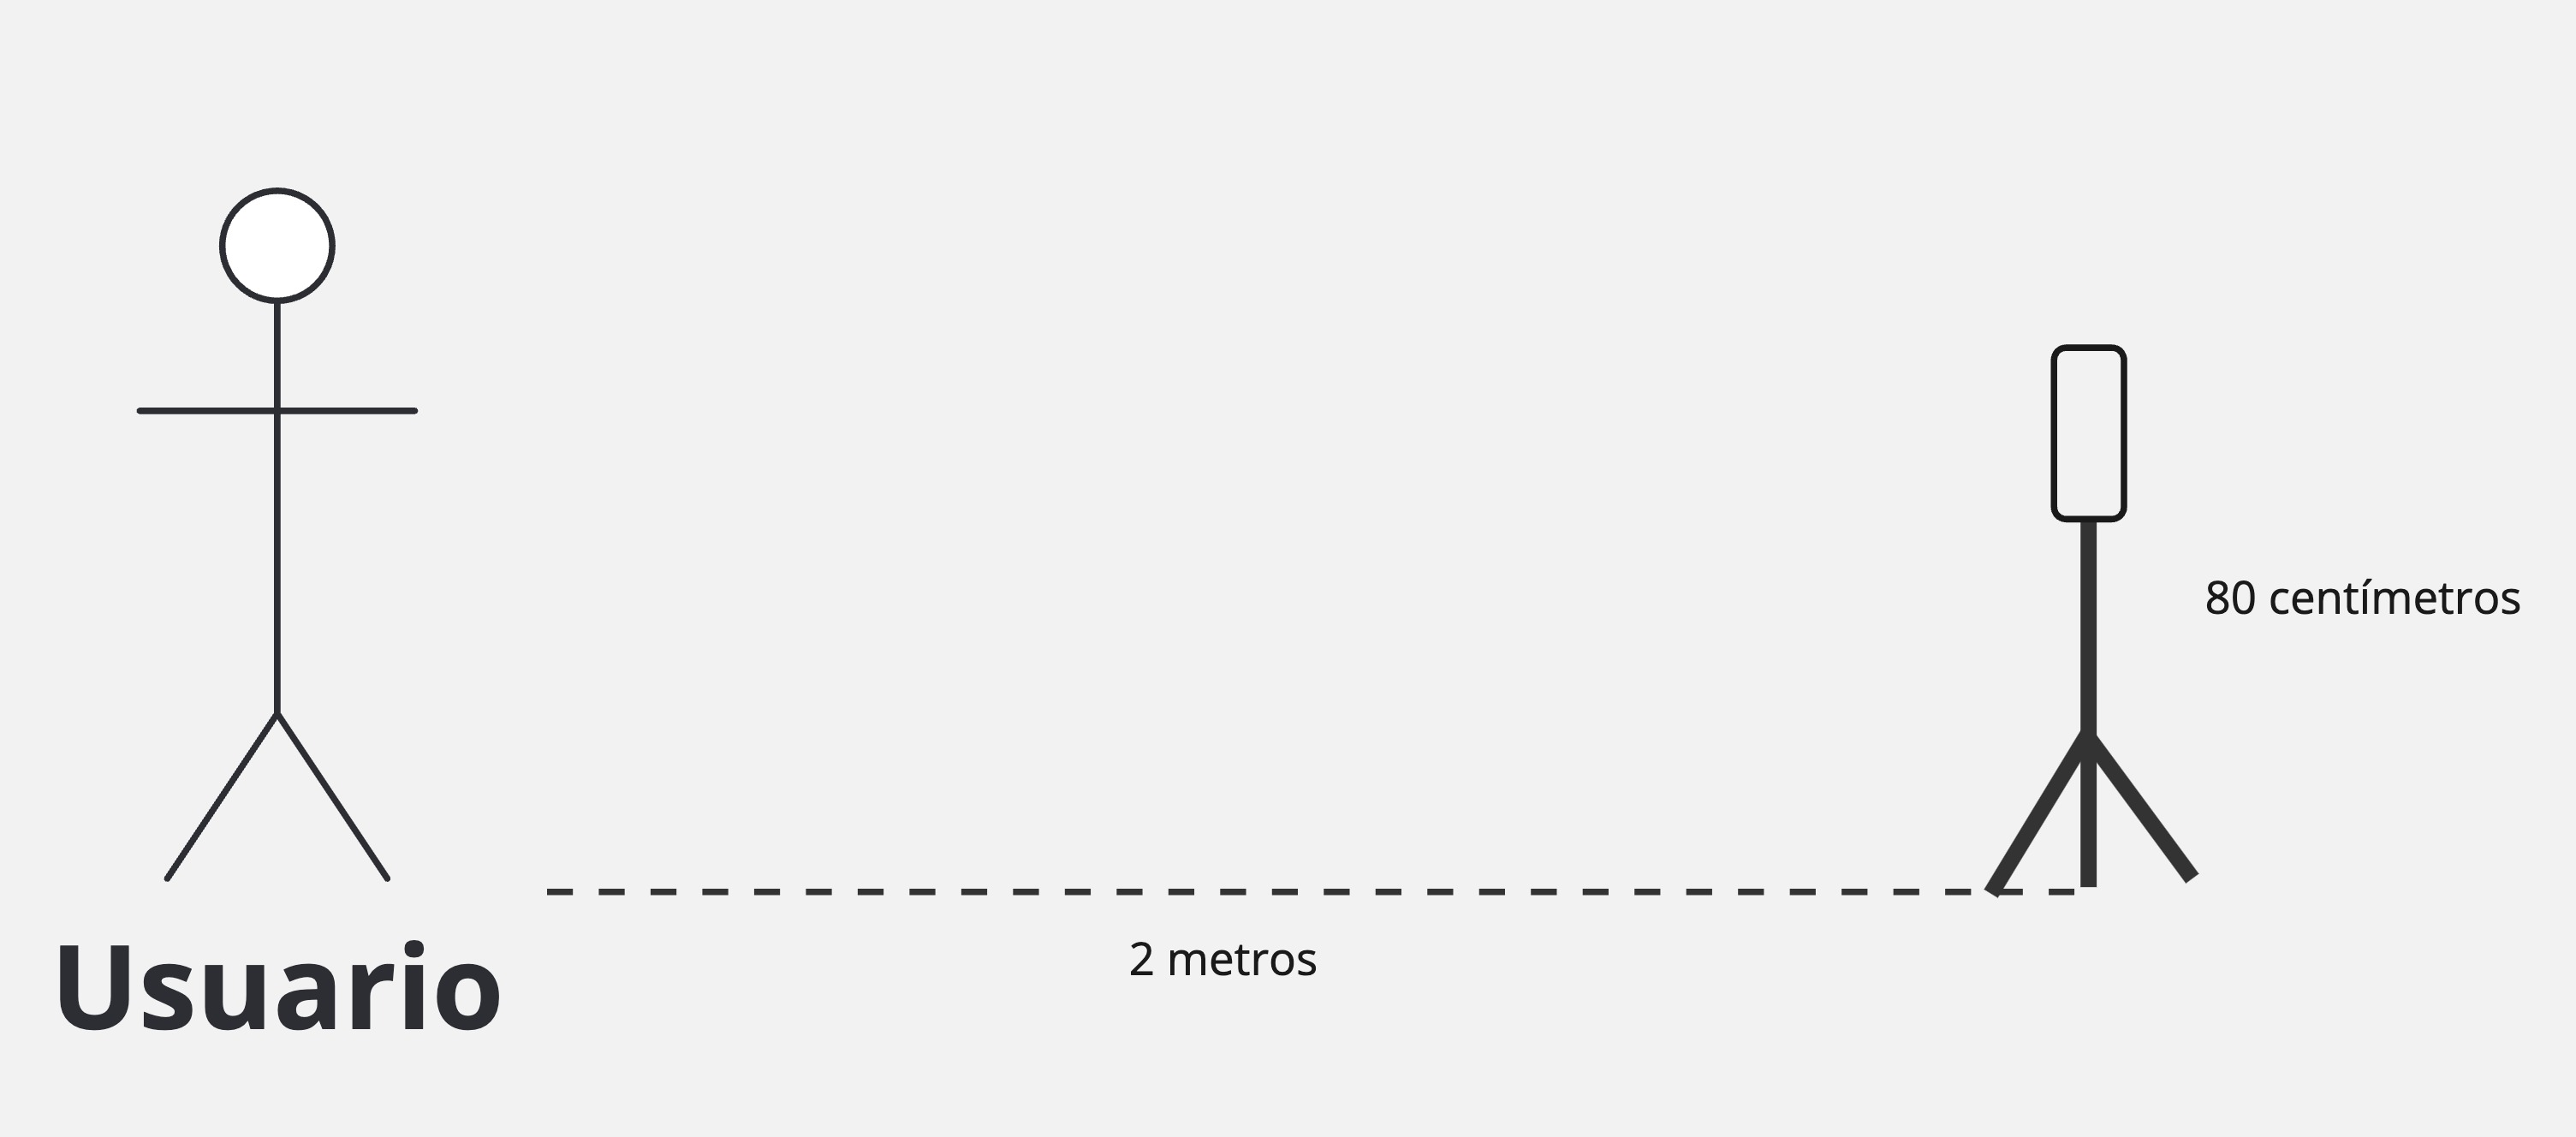
\includegraphics[width=0.48\linewidth]{2024_ConteoSentadillas/Ilustrativa.jpg}
\end{center}
\footfullcite*{\EntradaBibtex}
\end{frame}


\begin{frame}{\citetitle{\EntradaBibtex} (2)}
%\begin{block}{Pantallas Principales} 

\begin{columns}
% Column 1
\column{.5\linewidth}



\begin{center}
	\begin{tabular}{cc}
		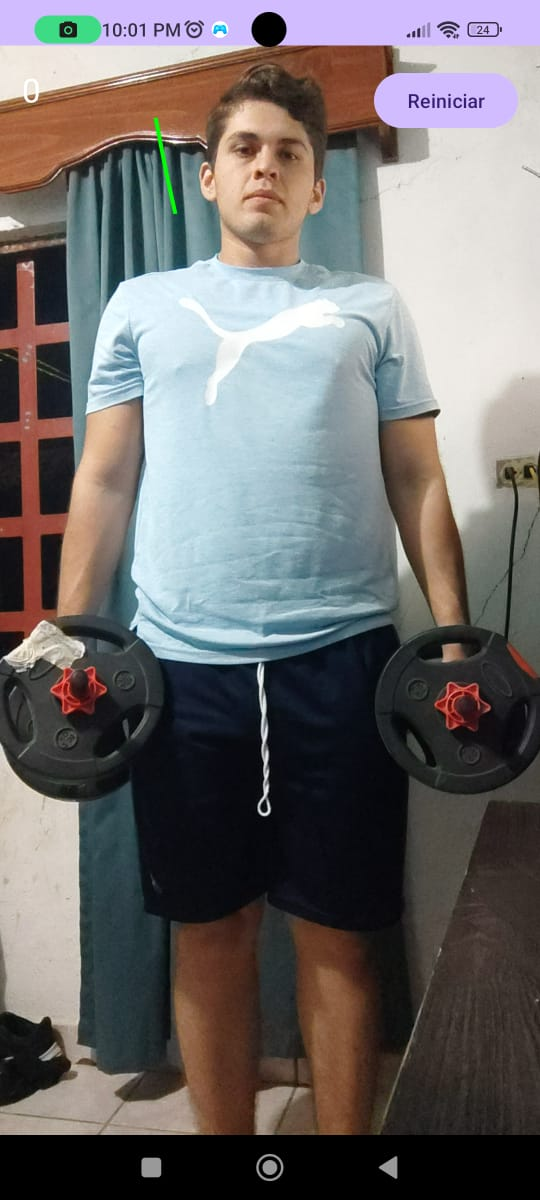
\includegraphics[width=0.40\linewidth]{2024_CurlBiceps/1.jpeg} &
		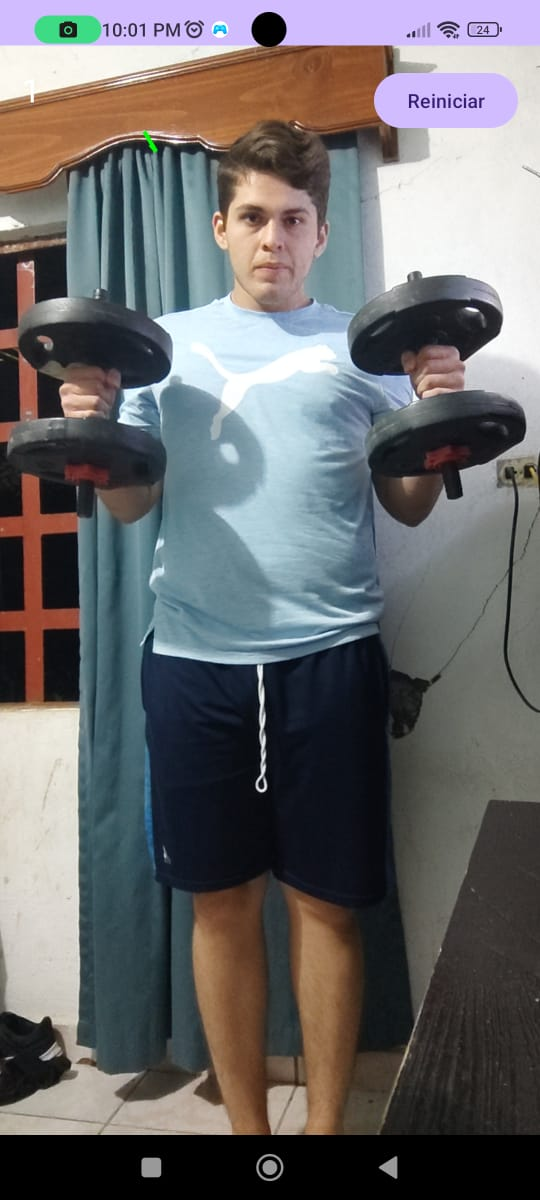
\includegraphics[width=0.40\linewidth]{2024_CurlBiceps/2.jpeg} \\
	\end{tabular}
\end{center}

\column{.5\linewidth}
\begin{center}
	\begin{tabular}{cccc}
		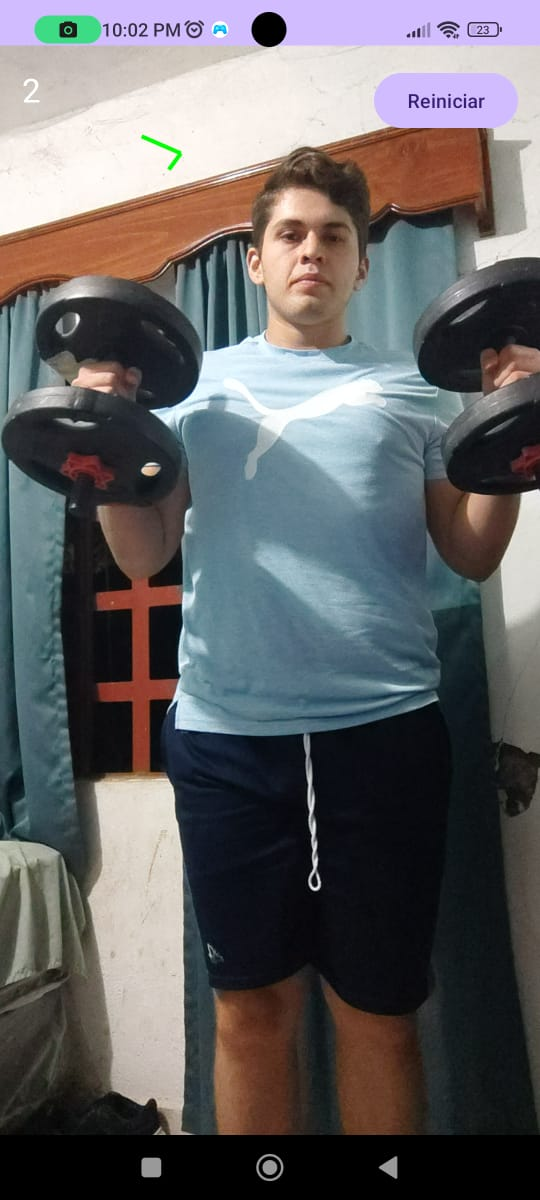
\includegraphics[width=0.40\linewidth]{2024_CurlBiceps/8.jpeg} &
 		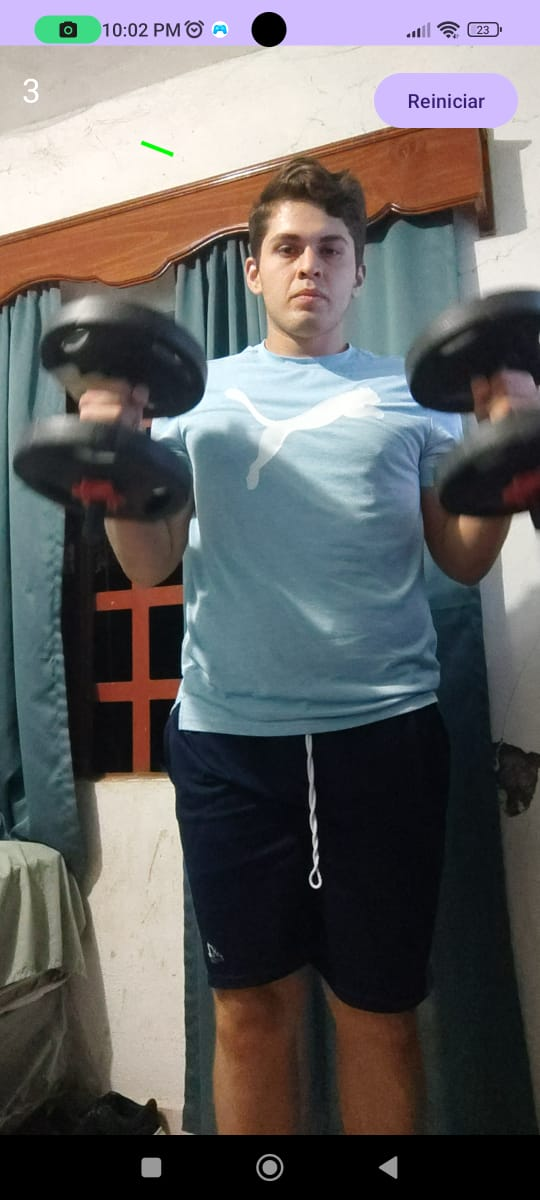
\includegraphics[width=0.40\linewidth]{2024_CurlBiceps/9.jpeg} \\
	\end{tabular}
\end{center}


\end{columns}
\end{frame}




\renewcommand{\EntradaBibtex}{AplicacionMovilManoRobotica_SistemasInteligentes_UPV_2023}


\begin{frame}{\citetitle{\EntradaBibtex} \footnotemark[1] (1)}
\begin{block}{Propuesta} 
Un modelo 3D dinámico de una Mano controlado por el usuario implementado en un teléfono inteligente
\end{block} 
\begin{itemize}
\item Utiliza la cámara del teléfono inteligente para detectar la mano (Libreria MediaPipe)
\item Utiliza OpenGL ES para crear el entorno 3D de una mano humana modelada en Blender
\item En base a los movimientos de los dedos del usuario, el modelo se actualiza
\end{itemize}
\footnotetext[1]{\fullcite{\EntradaBibtex}}
\end{frame}

\begin{frame}{\citetitle{\EntradaBibtex} (2)}

\begin{center}
	\begin{tabular}{ccc}
		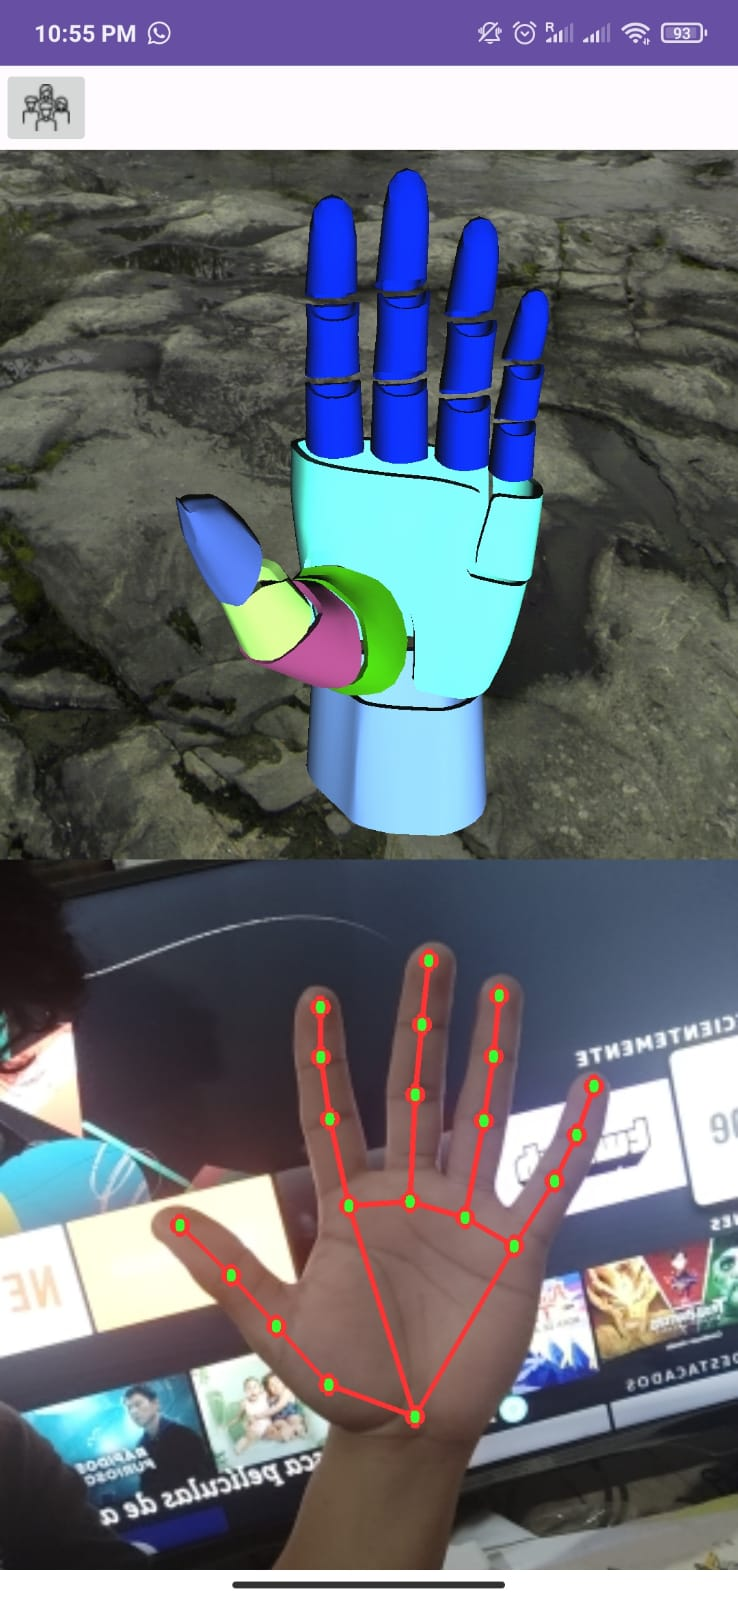
\includegraphics[width=0.20\linewidth]{2023_ManoRobotica/figs/hand01.jpeg} &
		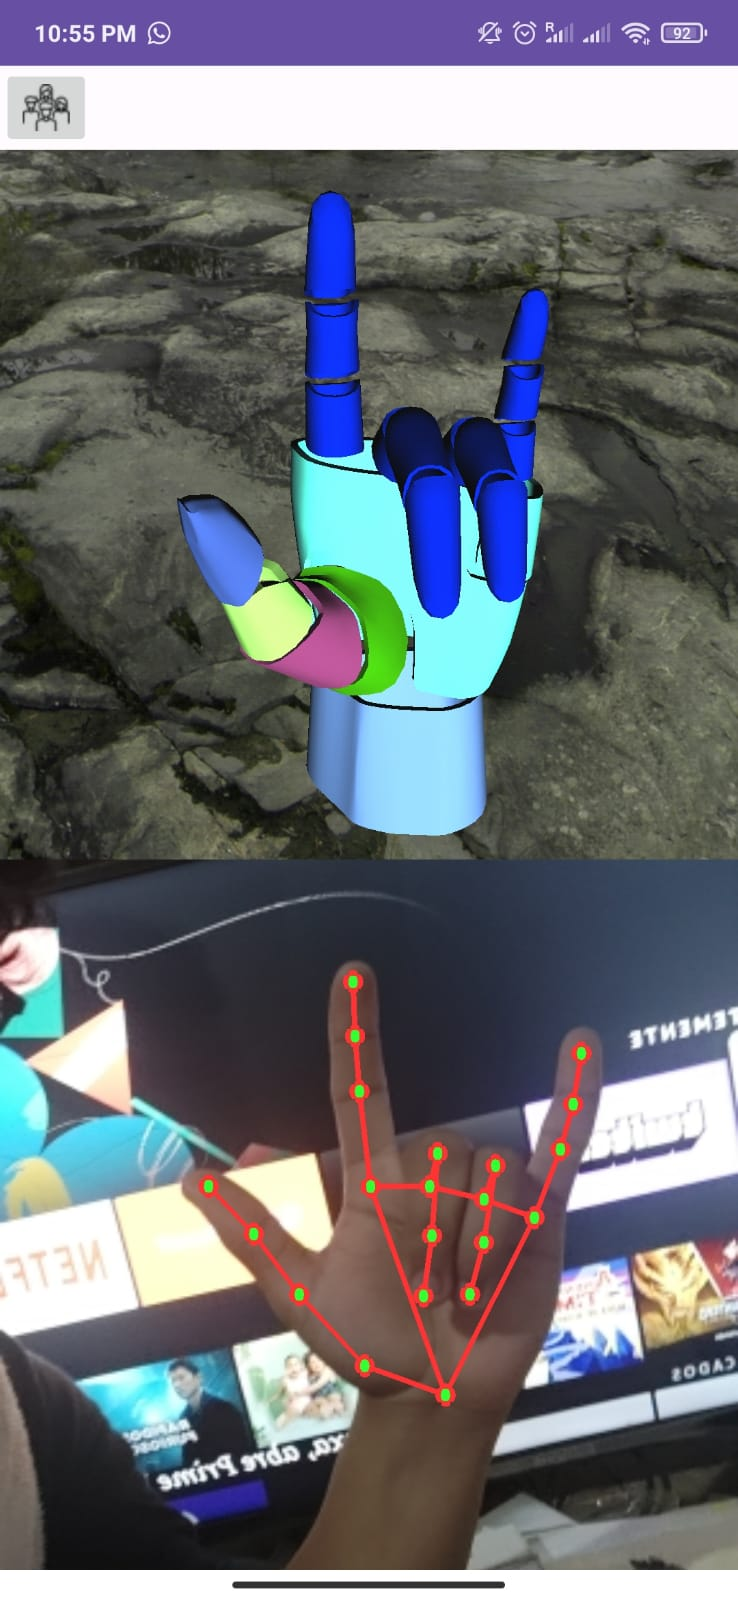
\includegraphics[width=0.20\linewidth]{2023_ManoRobotica/figs/hand02.jpeg} & 
		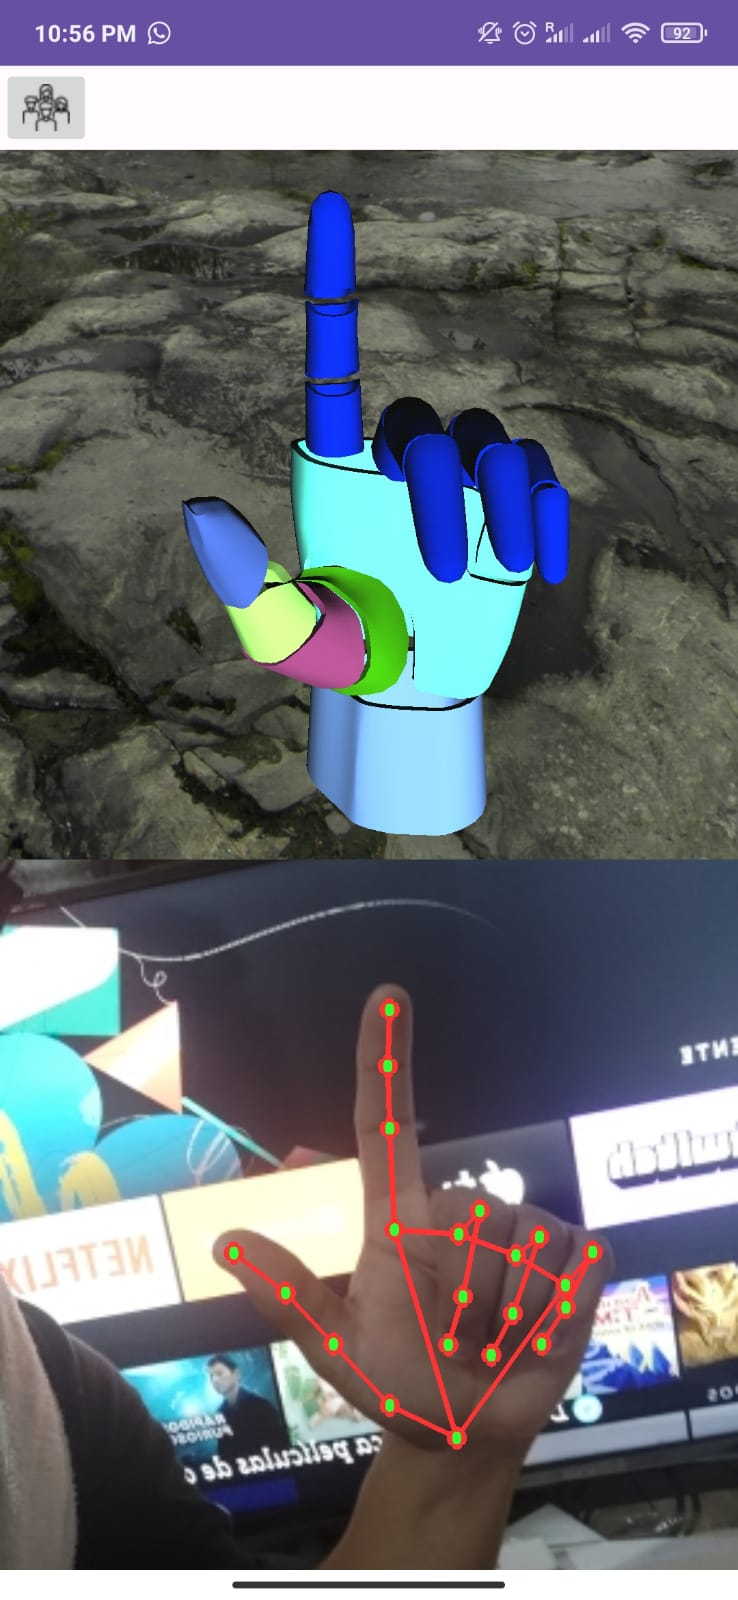
\includegraphics[width=0.20\linewidth]{2023_ManoRobotica/figs/hand03.jpeg}\\
	\end{tabular}
\end{center}

\end{frame}

%





\subsection{Realidad Aumentada}


\renewcommand{\EntradaBibtex}{RealidadAumentada_PrimerPrototipo_2019}
\begin{frame}{\citetitle{\EntradaBibtex} \footnotemark[1] (1)}

%\begin{frame}{Sistema de Realidad Aumentada \footnotemark}
%\begin{block}{Sistema de Realidad Aumentada \footnotemark} 
\begin{columns}
\begin{column}{0.48\textwidth}
		\begin{itemize}
		\item Detección de Codigos QR
		\item Decodificación del texto codificado en el codigo QR
		\item Sobreposición del modelo 3D dependiendo de la posición del código QR
		\end{itemize}
	\end{column}
	\begin{column}{0.52\textwidth}  
	    \begin{center}
	    	 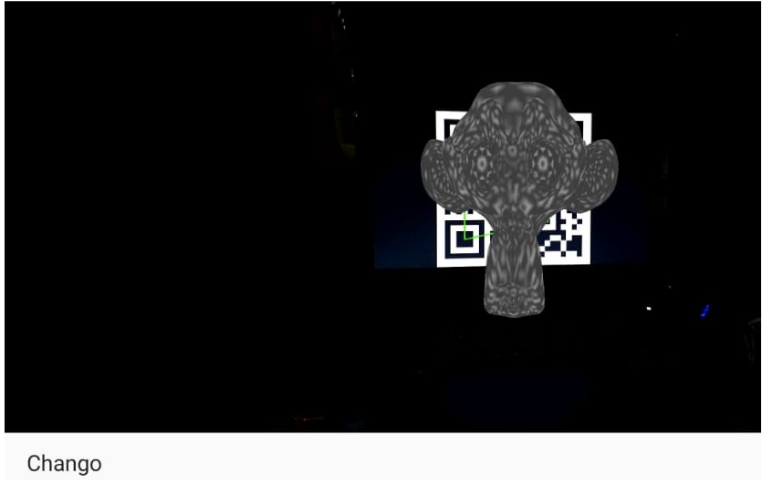
\includegraphics[width=0.95\textwidth]{Figs/SistemaAR1}
    	 \end{center}
	\end{column}
	\end{columns}
%	\end{block} 
\footnotetext[1]{\fullcite{\EntradaBibtex}}
%\footnotetext{Cárdenas Castillo Jesús Alfredo, Molina Pastrana Ana Karen, Ramos Lucio Eluis Carlo, Rodríguez Terán Linda Margarita y Vázquez Luna César Jovany.  \textbf{Visión por Computadora para Realidad Aumentada}. Universidad Politécnica de Victoria,  Informe técnico proyecto de asignatura ``Cómputo en Dispositivos Móviles'', 2019. Sin Publicar.}
%\\setcounter{footnote}{0}
\end{frame}

%Cárdenas Castillo Jesús Alfredo, Molina Pastrana Ana Karen, Ramos Lucio Eluis Carlo, Rodrı́guez Terán Linda Margarita, Vázquez Luna Cesar Jovany.
% \textbf{Visión por Computadora para Realidad Aumentada}. Universidad Politécnica de Victoria,  Informe técnico proyecto de asignatura ``Cómputo en Dispositivos Móviles'', 2019. Sin Publicar.

\begin{frame}{\citetitle{\EntradaBibtex} (2)}
%\begin{block}{Sistema de Realidad Aumentada (2)} 
\begin{columns}
\begin{column}{0.5\textwidth}
    \begin{center}
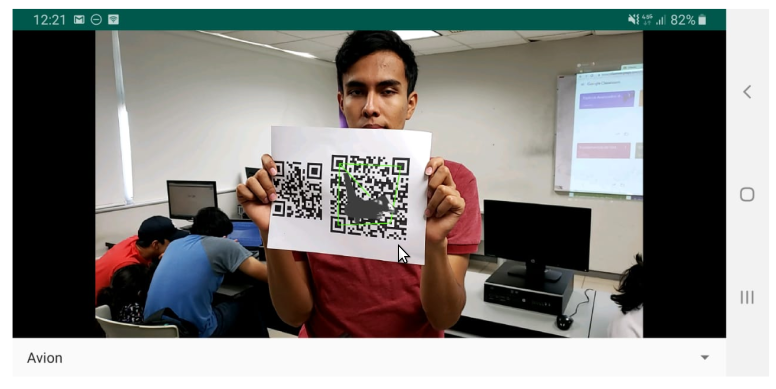
\includegraphics[width=0.98\textwidth]{Figs/SistemaAR2}\\
     \end{center}

\end{column}
\begin{column}{0.5\textwidth}  
    \begin{center}
\begin{itemize}
\end{itemize}

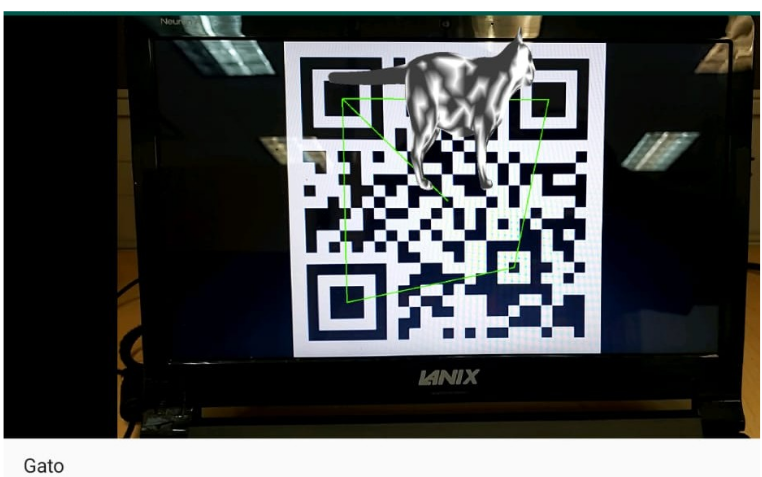
\includegraphics[width=0.98\textwidth]{Figs/SistemaAR3}\\
     \end{center}
\end{column}
\end{columns}



%\end{block} 
\end{frame}



\renewcommand{\EntradaBibtex}{MarcoNuno_Revista_2018_08_00}
\begin{frame}{\citetitle{\EntradaBibtex} \footnotemark[1] (1)}


%\begin{frame}{\citetitle{MarcoNuno_Revista_2018_08_00} \footnotemark (1)}
%\begin{block}{Aplicación para Enseñanza de Robótica utilizando Realidad Aumentada \footnotemark (1)} 
\begin{columns}
\begin{column}{0.5\textwidth}
Componentes:
		\begin{itemize}
		\item Un sistema (Arduino) que genera los movimientos del brazo robot incluye un transmisor Bluetooth
		\item Una aplicación móvil que visualizar un transportador virtual encima de una articulación robótica con el ángulo en tiempo real
		\end{itemize}
\end{column}
\begin{column}{0.5\textwidth}  
    \begin{center}
     %%%%% this is a minipage, so \textwidth is already adjusted to the size of the column
     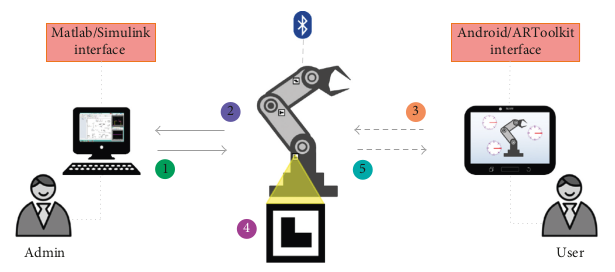
\includegraphics[width=0.9\textwidth]{Figs/SistemaAR_Maestria1}
     \end{center}
\end{column}
\end{columns}
%\end{block} 
\footnotetext[1]{\fullcite{\EntradaBibtex}}

\end{frame}

\begin{frame}{\citetitle{\EntradaBibtex} (2)}
%\begin{block}{Aplicación para Enseñanza de Robótica utilizando Realidad Aumentada (2)} 
\begin{columns}
\begin{column}{0.5\textwidth}
Funcionamiento de la aplicación:
		\begin{itemize}
		\item Se emplea un marcador ARUCO para determinar de que articulación se trata
		\item Mediante comandos Bluetooth se obtiene el ángulo
		\end{itemize}
\begin{center}
     %%%%% this is a minipage, so \textwidth is already adjusted to the size of the column
     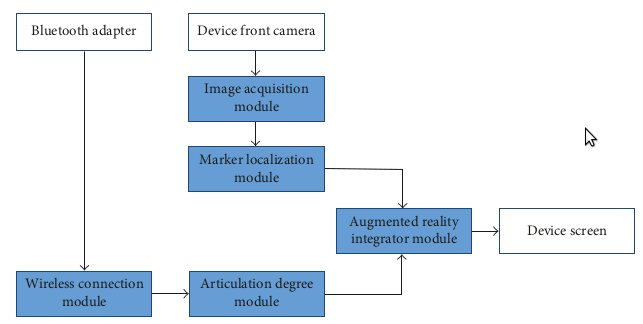
\includegraphics[width=0.79\textwidth]{Figs/SistemaAR_Maestria2}
     \end{center}
\end{column}
\begin{column}{0.5\textwidth}  
    \begin{center}
     %%%%% this is a minipage, so \textwidth is already adjusted to the size of the column
     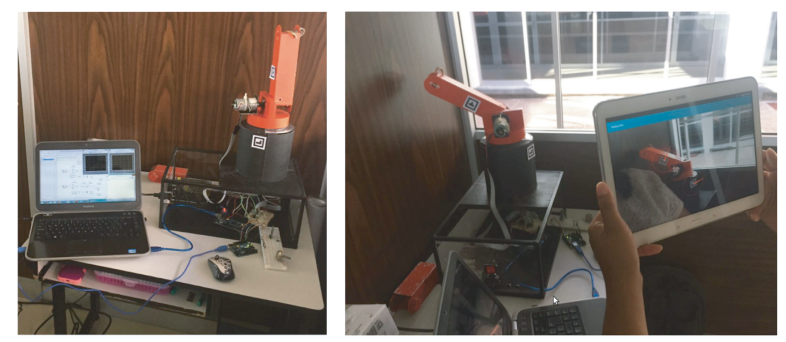
\includegraphics[width=0.79\textwidth]{Figs/SistemaAR_Maestria3}
     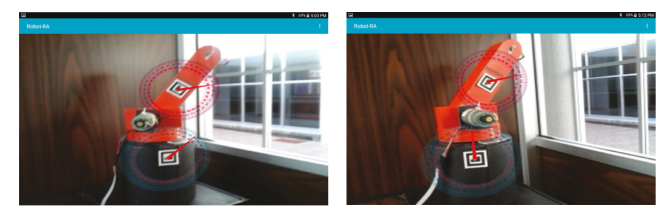
\includegraphics[width=0.79\textwidth]{Figs/SistemaAR_Maestria4}
     \end{center}
\end{column}
\end{columns}
%\end{block} 
\end{frame}




\renewcommand{\EntradaBibtex}{MapaRealidadVirtual_UPV_2022}
						 
\begin{frame}{\citetitle{\EntradaBibtex} \footnotemark[1] (1)}
\begin{columns}
\begin{column}{0.99\textwidth}
	\begin{itemize}
		\item Se propone una aplicación de RA que despliegue un MAPA de la UPV
		\item Se generó el modelo utilizando Blender y se exportó a un formato GLB
		\item La aplicación hace uso de la cámara para desplegar el modelo en una superficie con textura
	\end{itemize}
\end{column}
\begin{column}{0.01\textwidth}  
\begin{center}
     \begin{tabular}{c}
%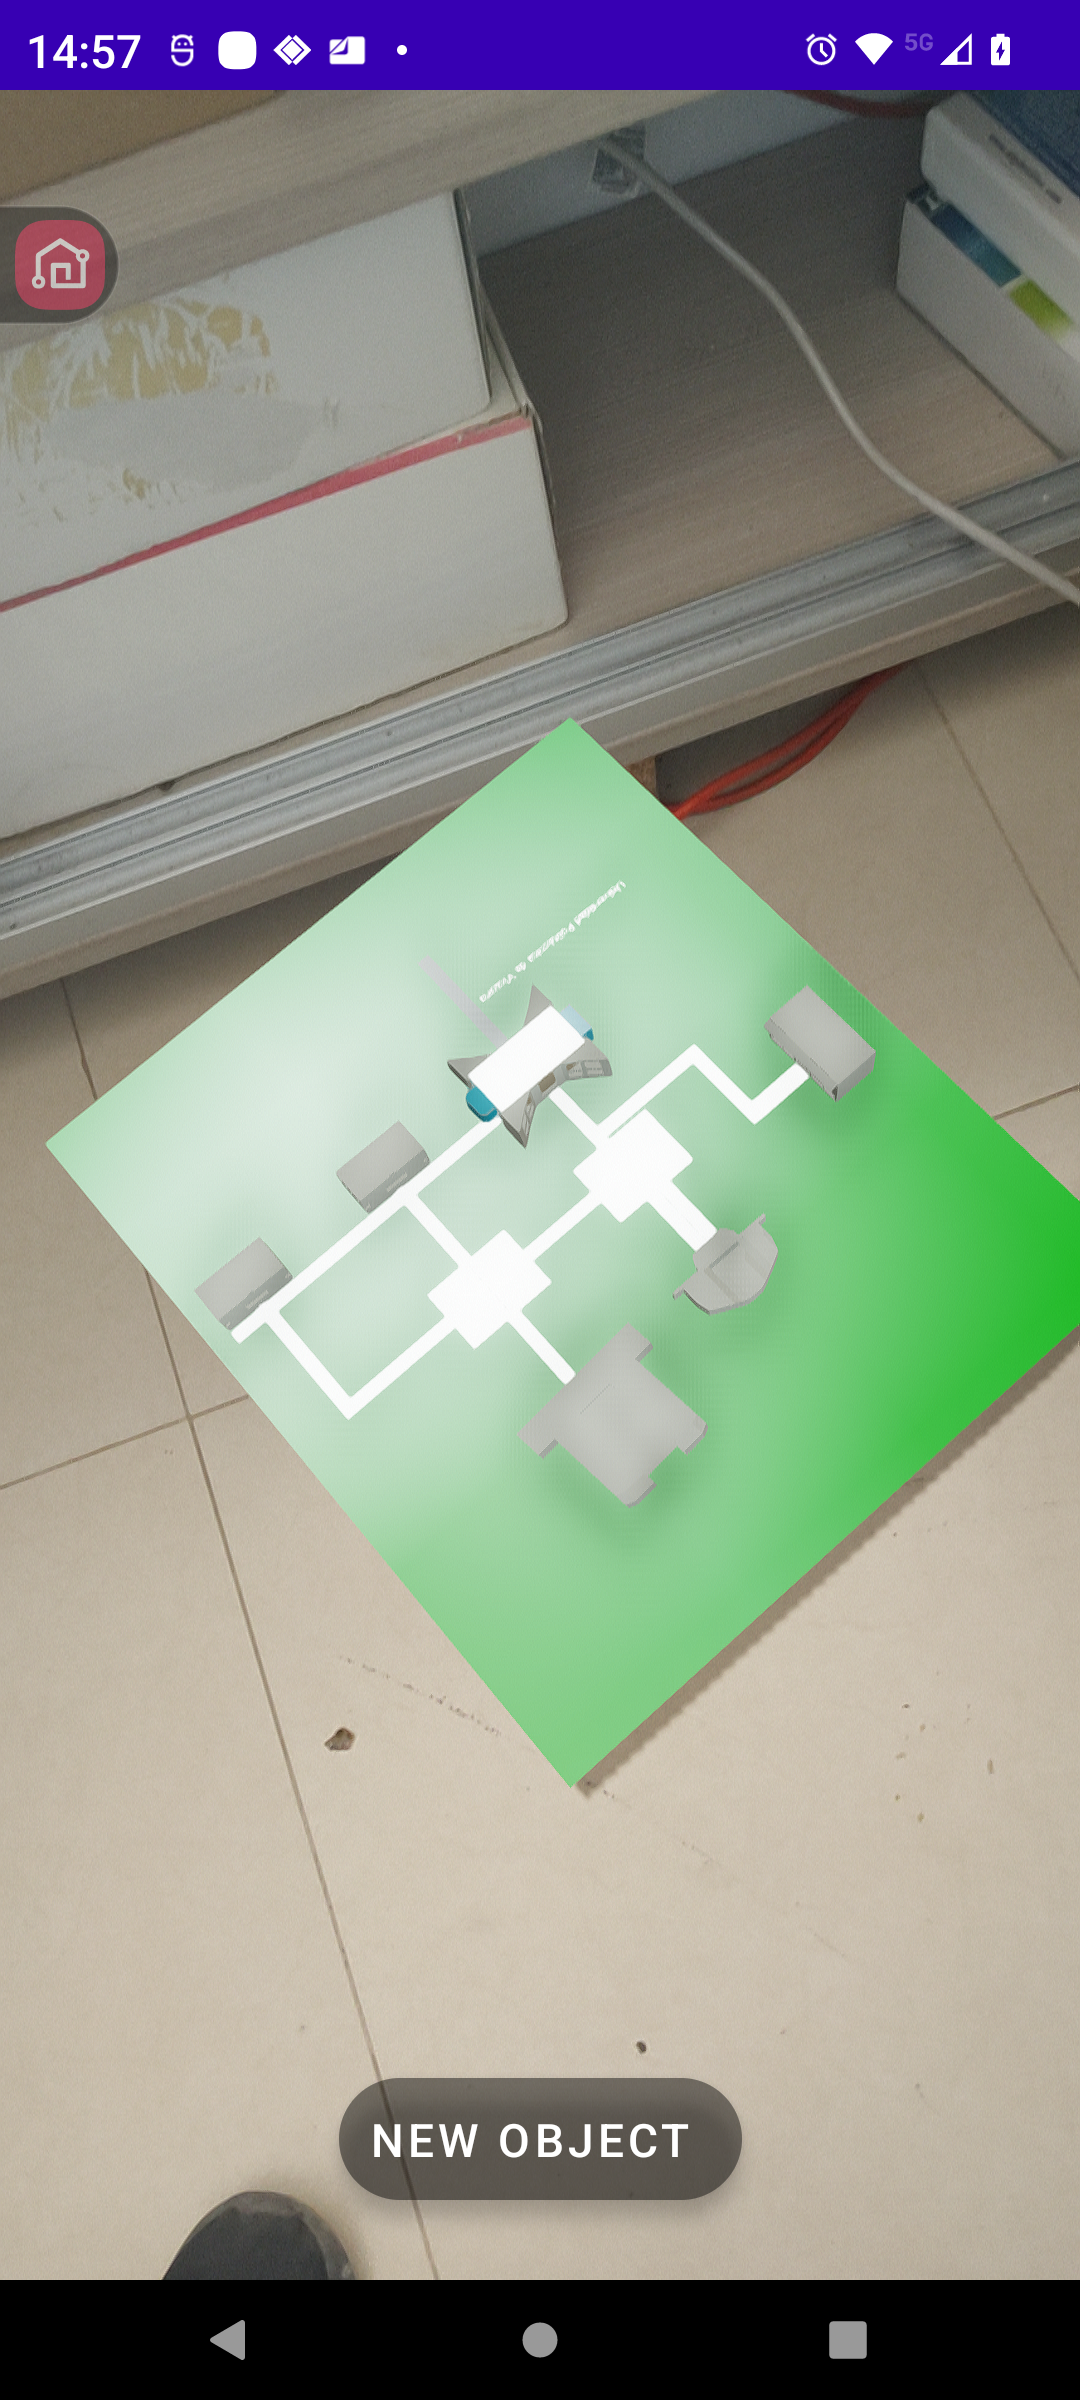
\includegraphics[width=0.48\textwidth]{2022_MapaUPV_RealidadAumentada/figs/MapaUPV_01}
%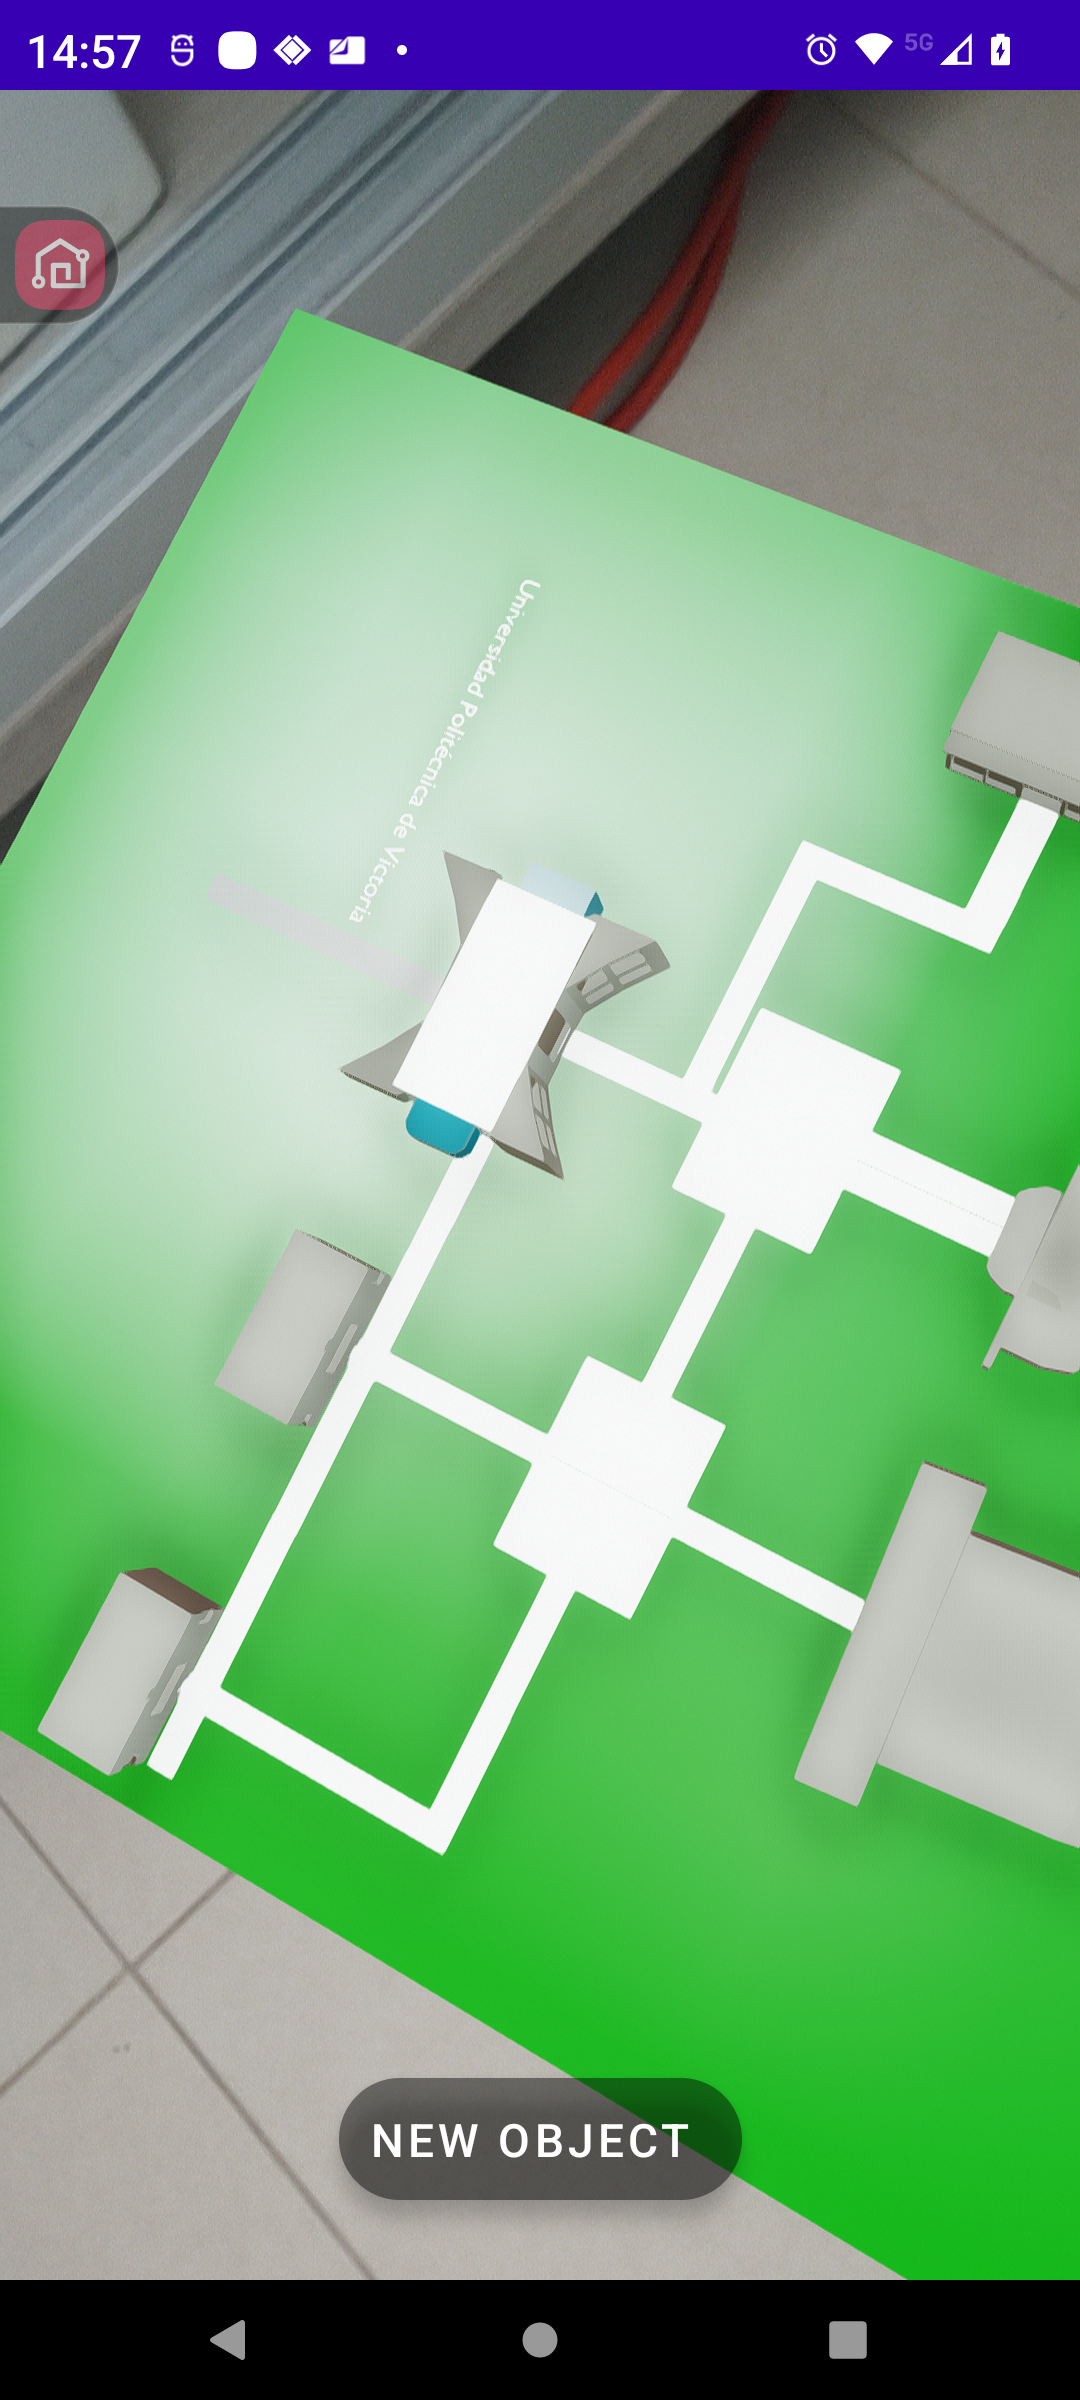
\includegraphics[width=0.48\textwidth]{2022_MapaUPV_RealidadAumentada/figs/MapaUPV_02}\\         
      \end{tabular}
\end{center}
\end{column} 
\end{columns} 
\footnotetext[1]{\fullcite{\EntradaBibtex}}
\end{frame}


\begin{frame}{\citetitle{\EntradaBibtex} (2)}
\begin{columns}
\begin{column}{0.4\textwidth}
	\begin{itemize}
		\item Se propone una aplicación de RA que despliegue un MAPA de la UPV
	\end{itemize}
\end{column}
\begin{column}{0.6\textwidth}  
\begin{center}
     \begin{tabular}{c}
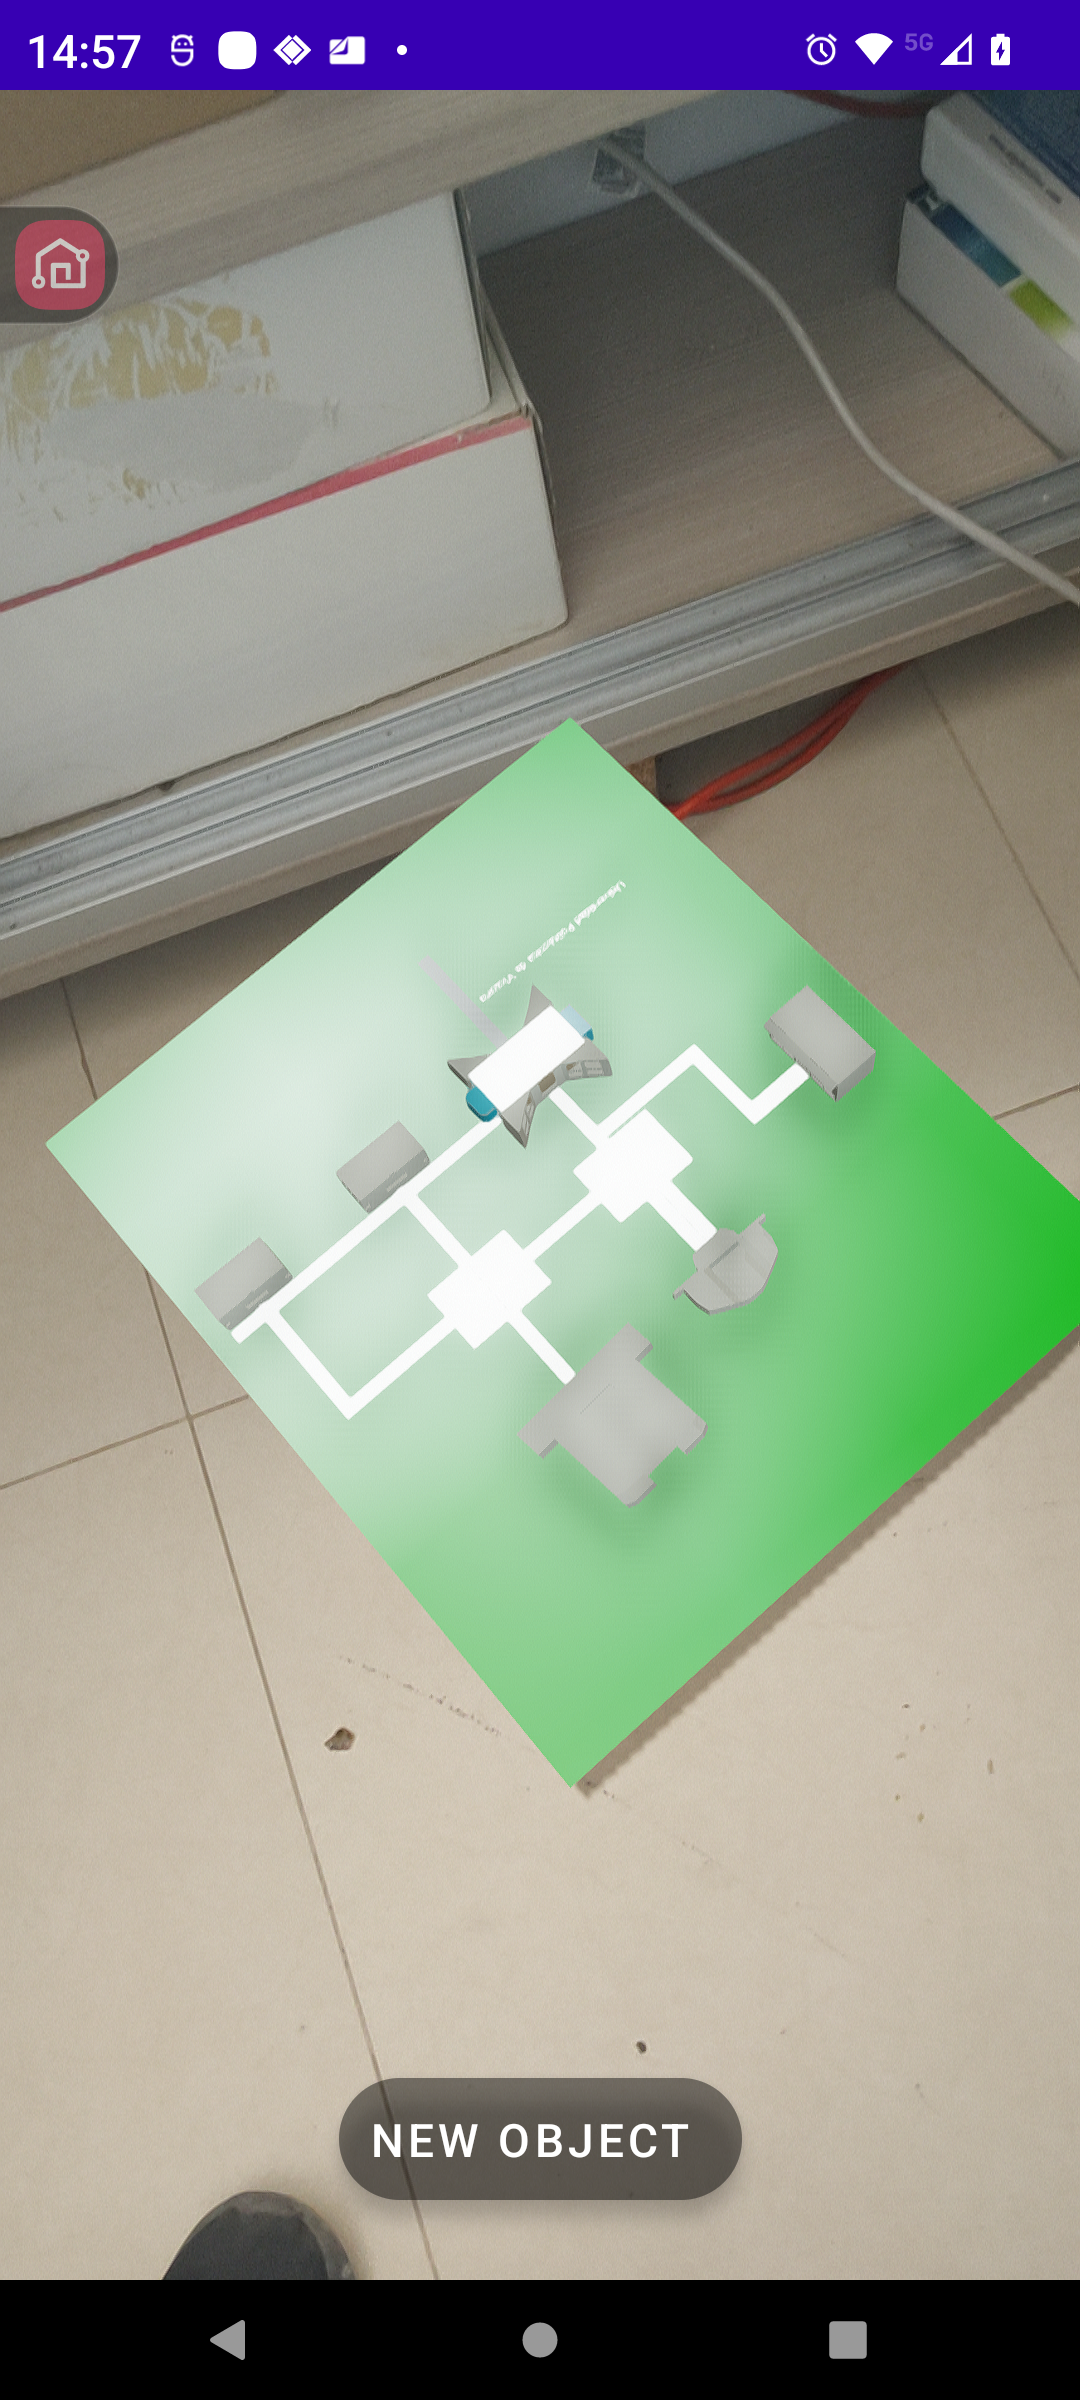
\includegraphics[width=0.24\textwidth]{2022_MapaUPV_RealidadAumentada/figs/MapaUPV_01}
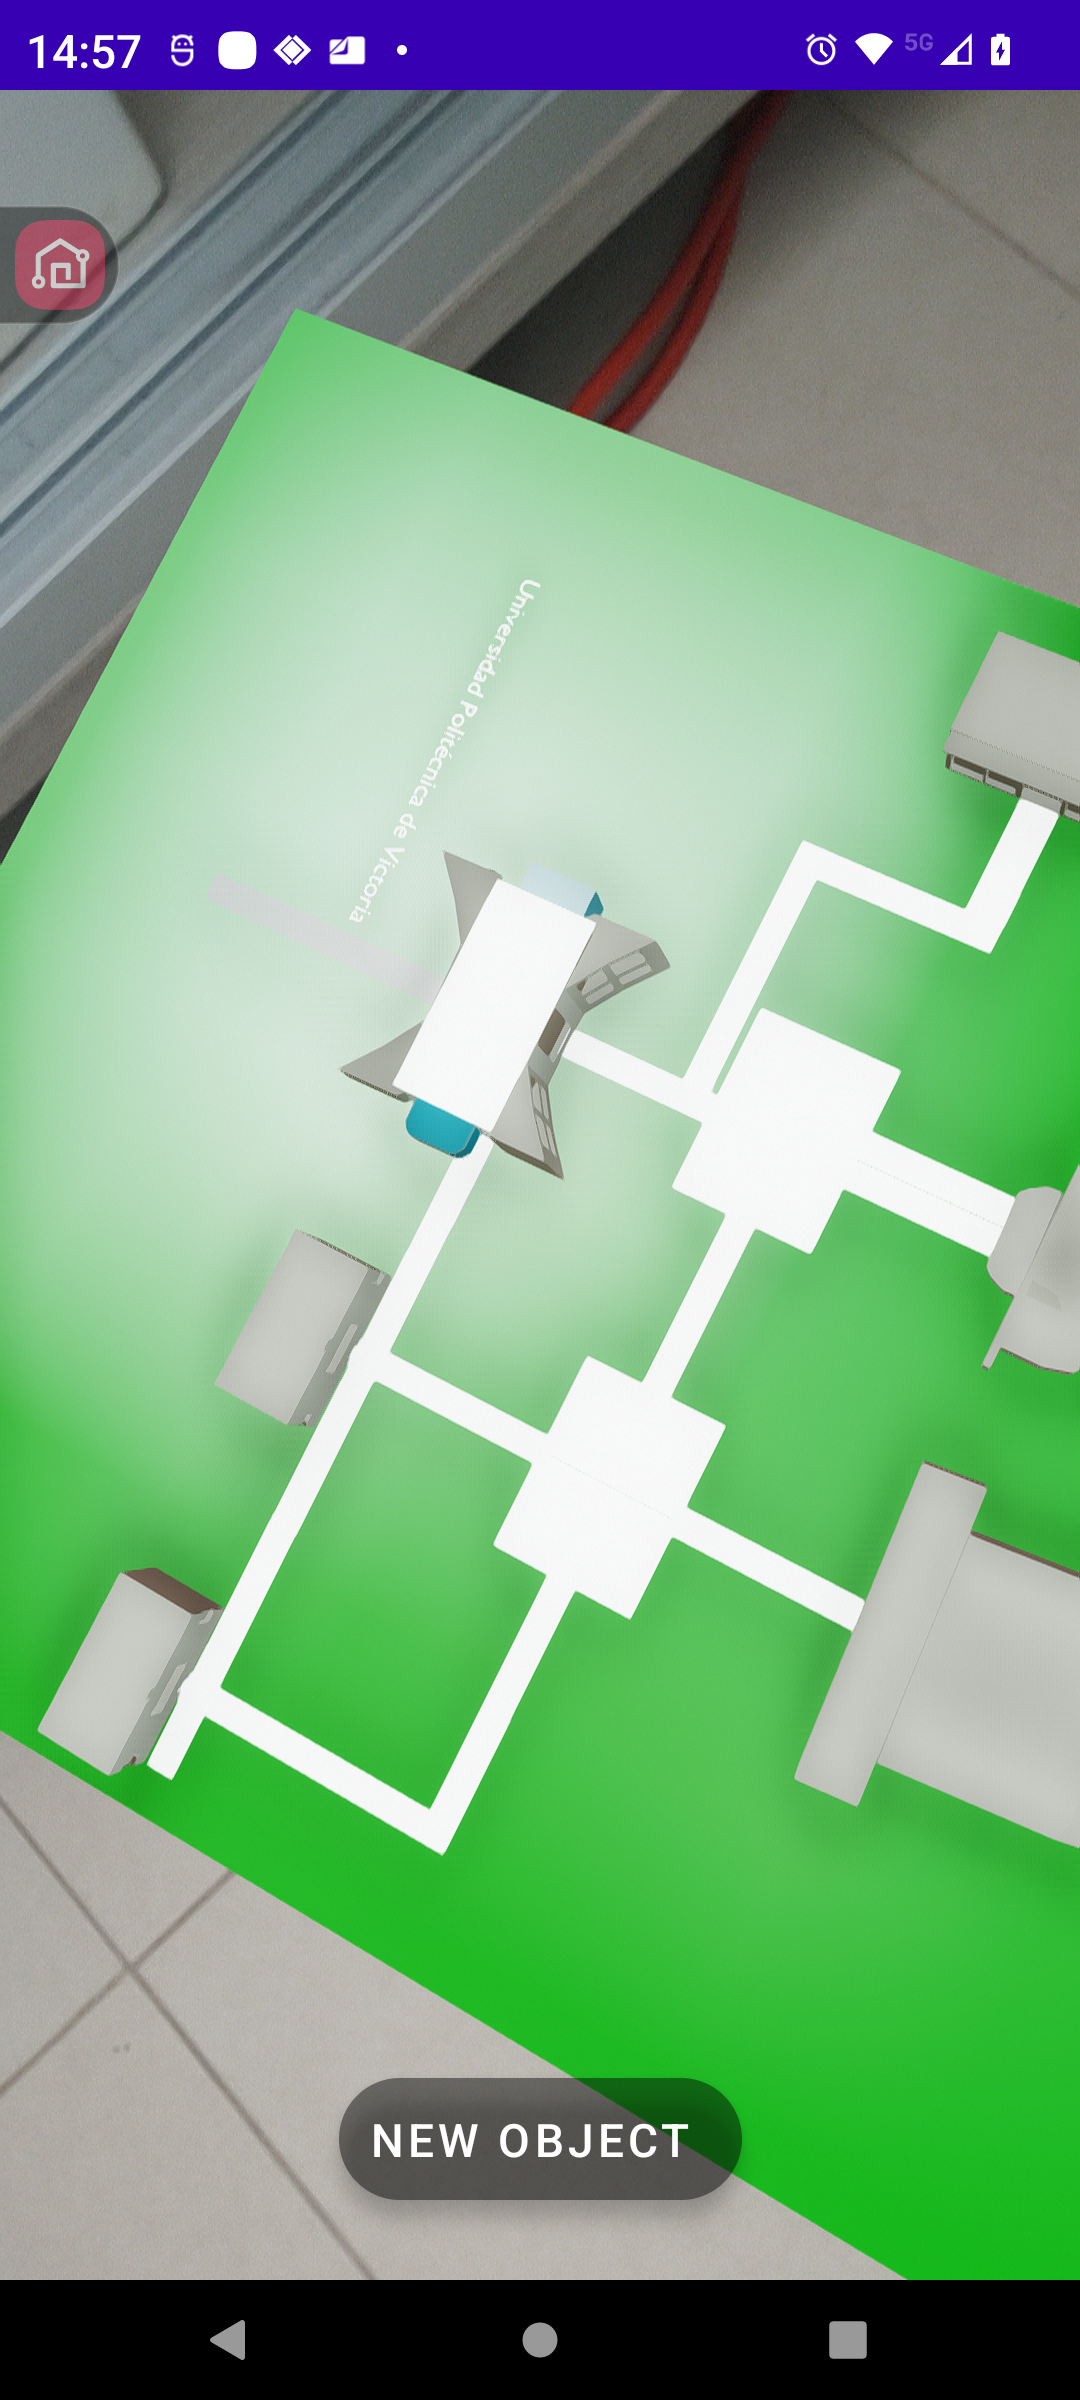
\includegraphics[width=0.24\textwidth]{2022_MapaUPV_RealidadAumentada/figs/MapaUPV_02}
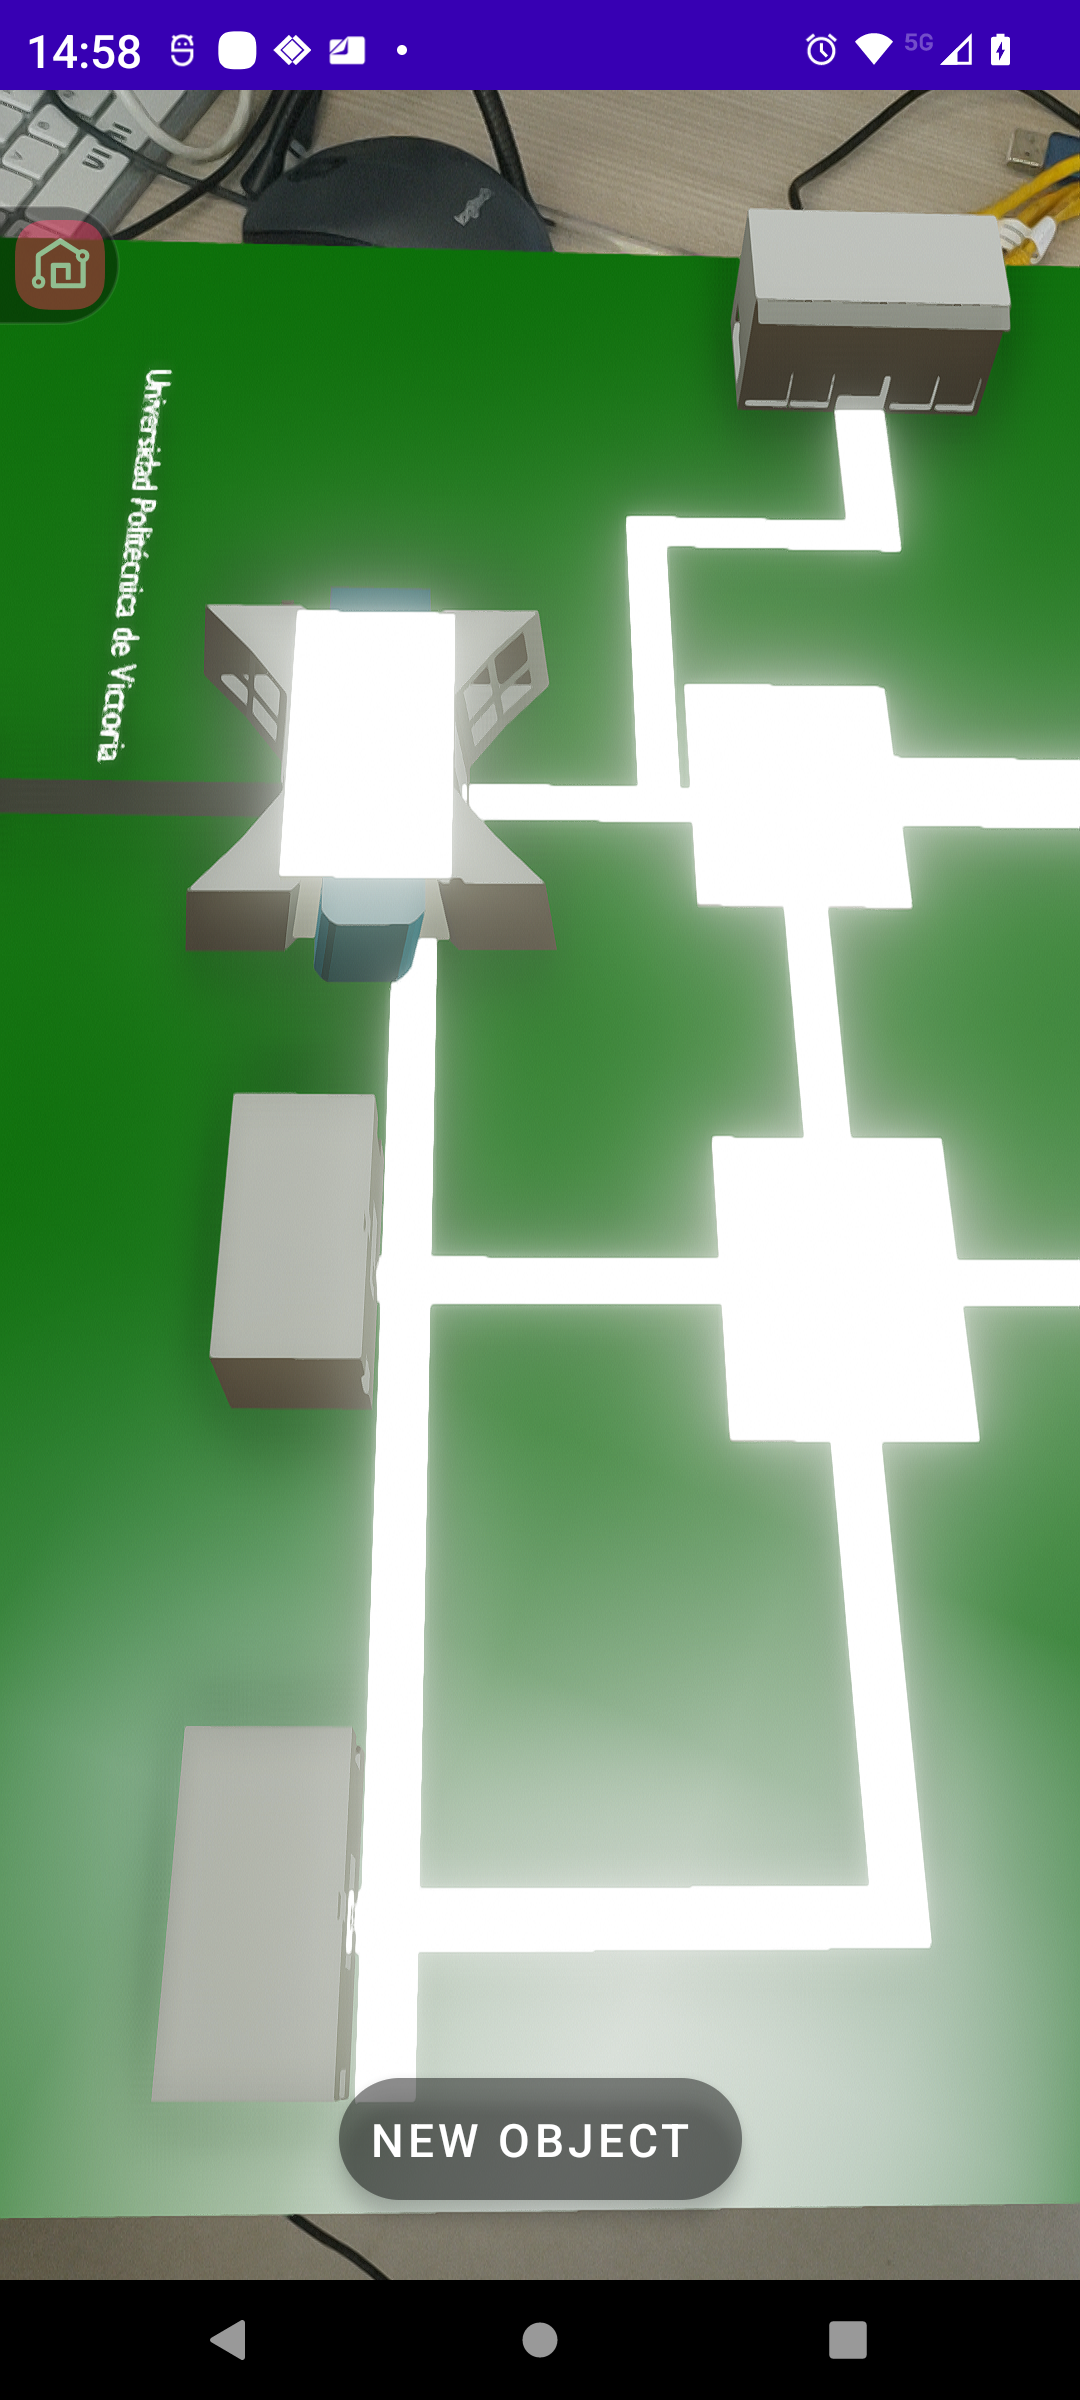
\includegraphics[width=0.24\textwidth]{2022_MapaUPV_RealidadAumentada/figs/MapaUPV_03}
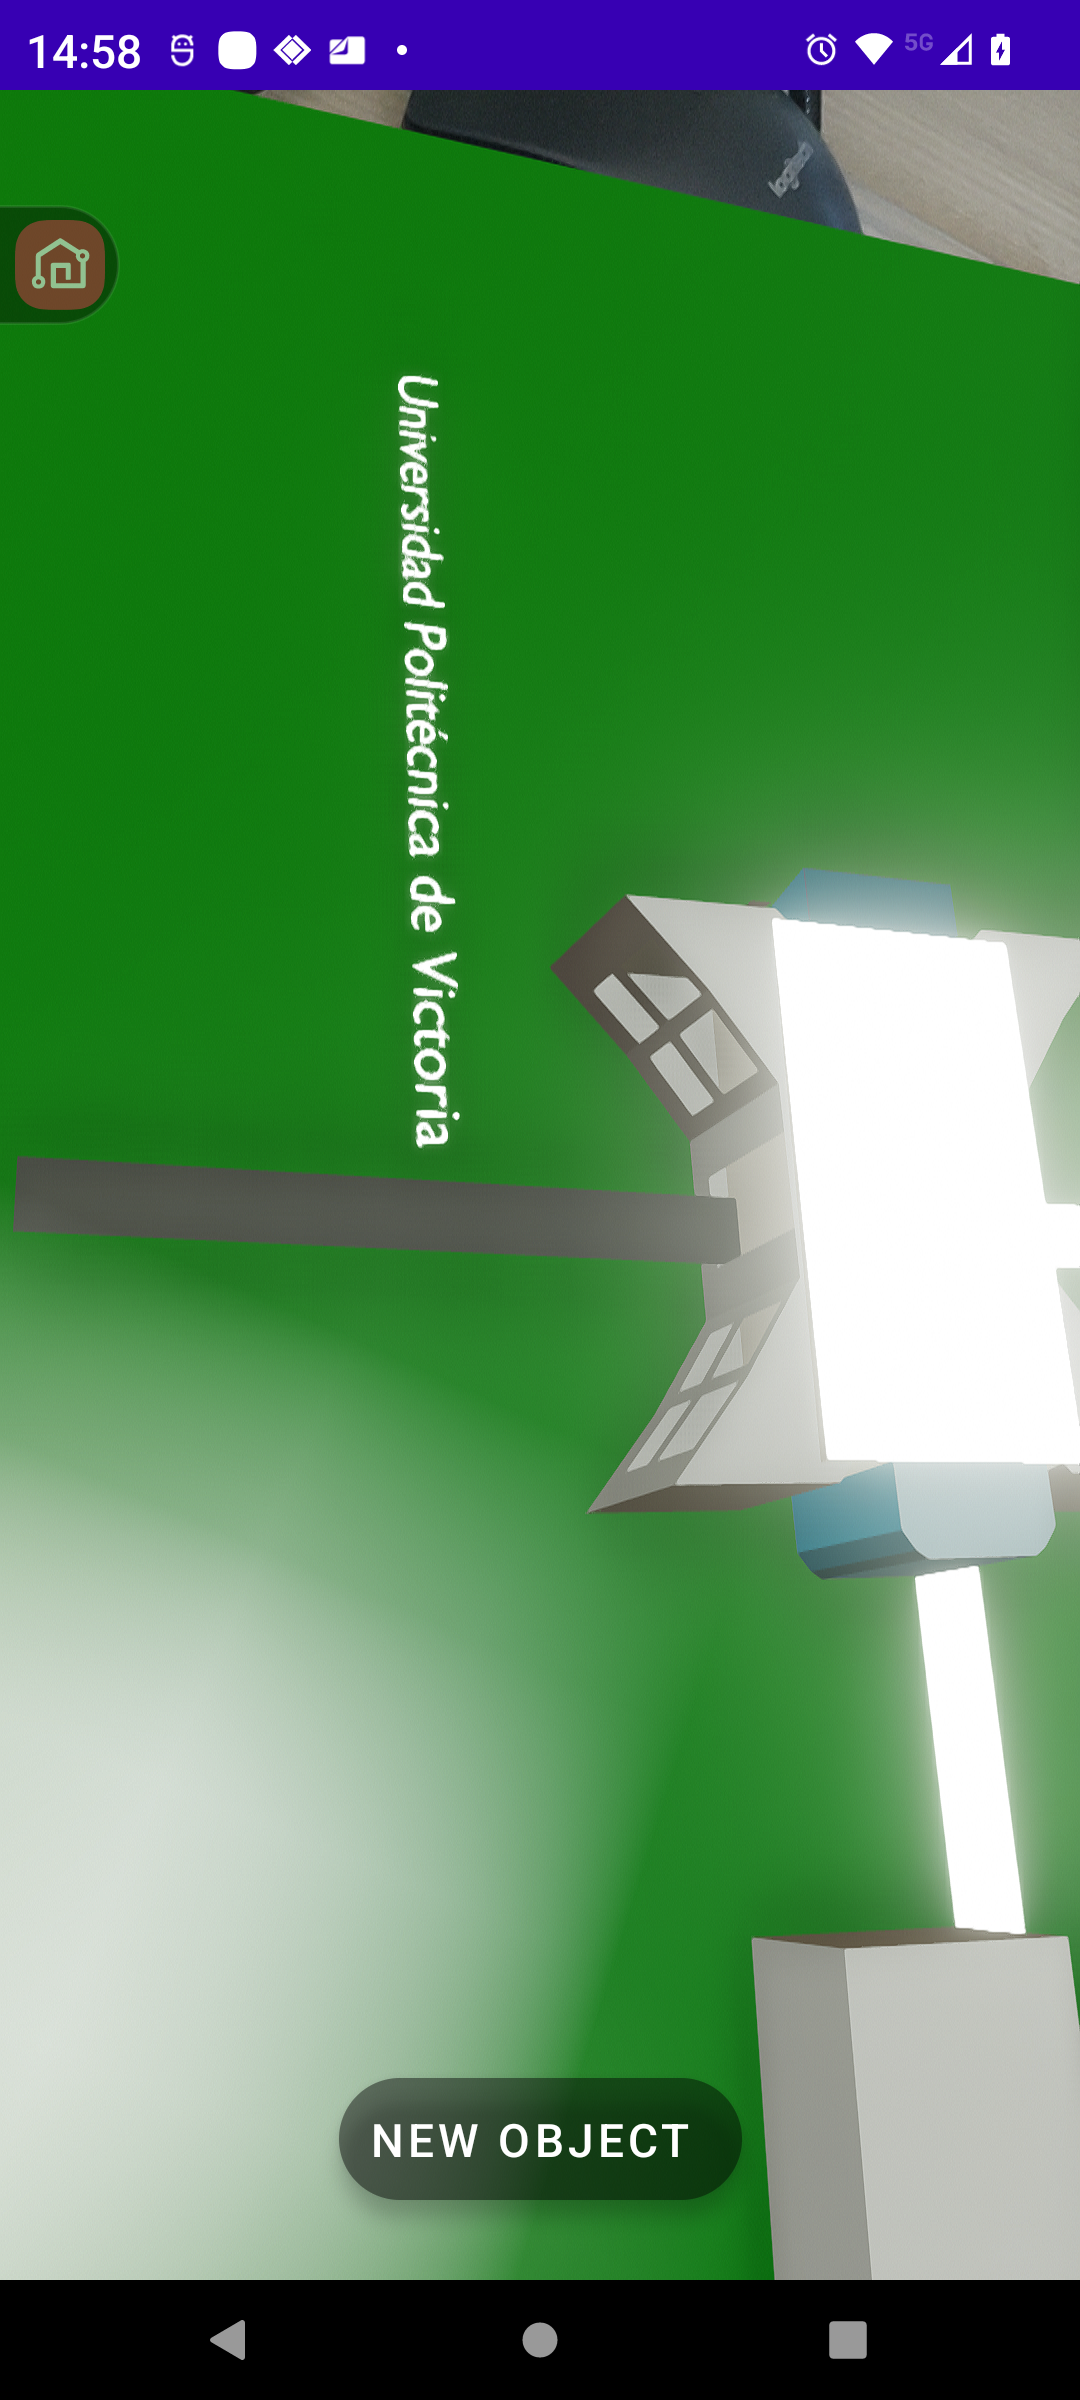
\includegraphics[width=0.24\textwidth]{2022_MapaUPV_RealidadAumentada/figs/MapaUPV_04}\\         
      \end{tabular}
\end{center}
\end{column} 
\end{columns} 

\end{frame}







\renewcommand{\EntradaBibtex}{CabezaJaguar_2023}
\begin{frame}{\citetitle{\EntradaBibtex} \footnotemark[1] (1)}
%\begin{block}{Brazo Robótico \footnotemark} 
\begin{columns}
	\begin{column}{0.55\textwidth}
		\begin{itemize}
			\item La mascota institucional de la UPV es el Jaguar
			\item Se diseño un filtro que detecta el rostro de una persona y sobrepone la imagen de un Jaguar
		\end{itemize}
	\end{column}
	\begin{column}{0.22\textwidth}
		 \begin{center}
		     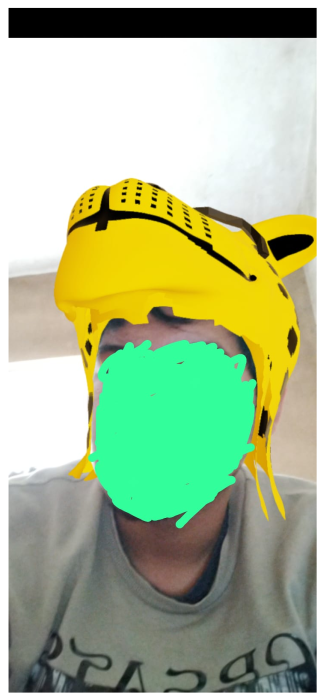
\includegraphics[width=0.98\textwidth]{2025_CabezaJaguarUPV/figs/Jaguar1}
		 \end{center}
	\end{column}
	\begin{column}{0.22\textwidth}  
		\begin{center}
		 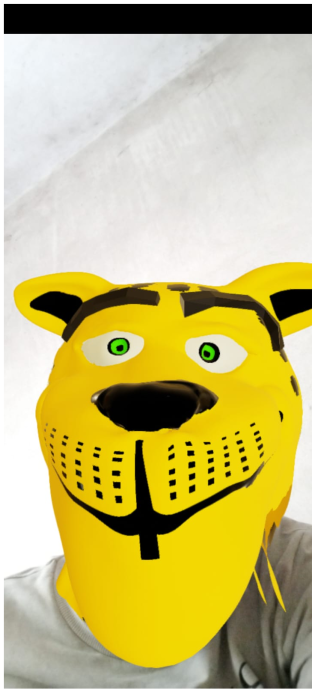
\includegraphics[width=0.98\textwidth]{2025_CabezaJaguarUPV/figs/Jaguar2}
		 \end{center}
	\end{column}
\end{columns}
%\end{block} 
\footnotetext[1]{\fullcite{\EntradaBibtex}}
\end{frame}



\renewcommand{\EntradaBibtex}{virtualworlds5040053}

\begin{frame}{\citetitle{\EntradaBibtex} \footnotemark[1] (1)}
Visualización de materiales híbridos multifuncionales
\begin{itemize}
\item Los materiales híbridos pueden integrar múltiples fases activas dentro de una misma estructura.
\item Su comportamiento depende de la interacción entre diferentes componentes.
\item Los diagramas 2D tradicionales dificultan comprender:
\begin{itemize}
  \item La distribución espacial de los componentes.
  \item La relación entre estructura y función.
  \item Los mecanismos de interacción.
\end{itemize}
\item Se propone utilizar visualización 3D interactiva y realidad aumentada (RA) para mejorar la comunicación científica, la cual permite explorar la estructura de un material complejo de una manera más intuitiva.
\end{itemize}
%La visualización inmersiva permite explorar la estructura de un material complejo de una manera más intuitiva que una representación estática.
\footnotetext[1]{\fullcite{\EntradaBibtex}}
\end{frame}

\begin{frame}{\citetitle{\EntradaBibtex} (2)}

Multifunctional Hybrid Material (MHM-App)

La aplicación representa una esfera multifuncional formada por:
\begin{itemize}
\item TiO$_2$: fase fotocatalítica.
\item Fe$_3$O$_4$ (magnetita): fase magnética.
\item Carbón activado: material adsorbente.
\item Clinoptilolita con hipoclorito: agente de liberación/control.
\item CuO: componente con función antimicrobiana.
\item Alginato de sodio: matriz encapsulante formada mediante gelación iónica.
\item Quitosano reticulado: recubrimiento externo.
\end{itemize}
La aplicación permite observar simultáneamente la estructura global y los diferentes materiales que la constituyen.
\end{frame}



\begin{frame}{\citetitle{\EntradaBibtex} (3)}

Aplicación móvil de visualización 3D + RA, proporciona dos modos complementarios:

\begin{columns}

% Column 1
\column{.4\linewidth}

\item Modo Realidad Aumentada
\begin{itemize}
\item Detecta una superficie horizontal.
\item Utiliza raycasting para colocar la esfera.
\item Permite observar el material integrado en el entorno real.
\end{itemize}

\column{.6\linewidth}
\begin{center}
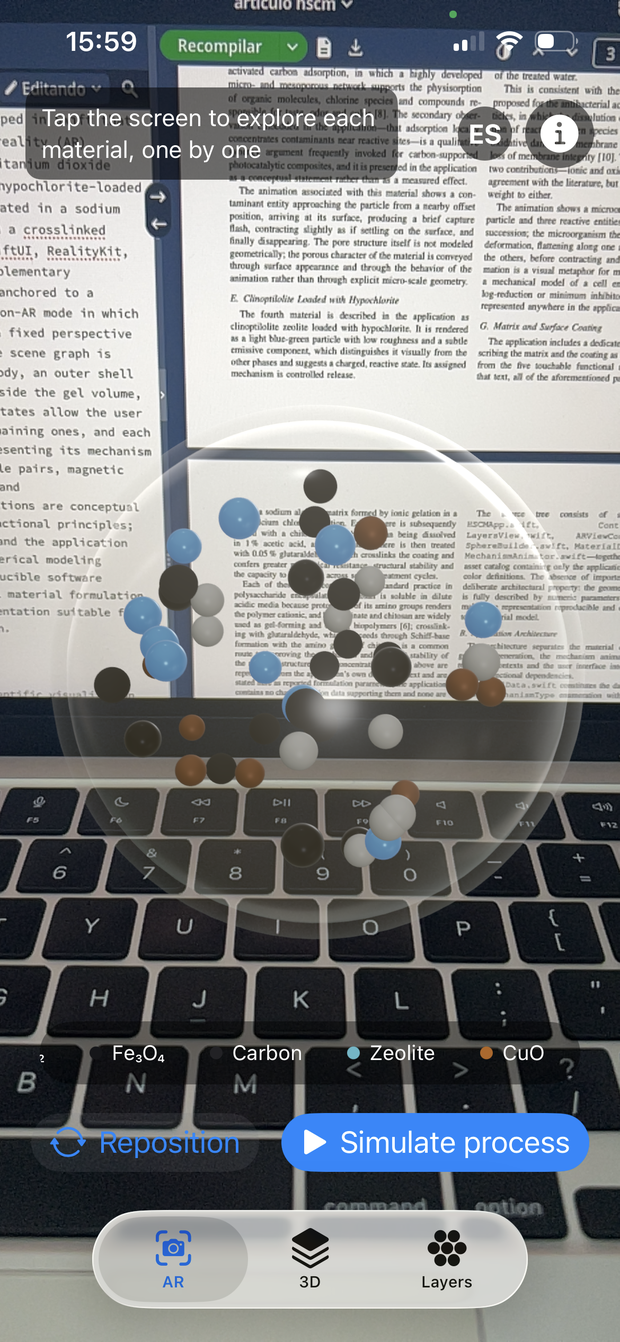
\includegraphics[width=0.20\linewidth]{2026_Augmented_Reality_Multifunctional_Hybrid_Materials/figs/hscm1_en.PNG}
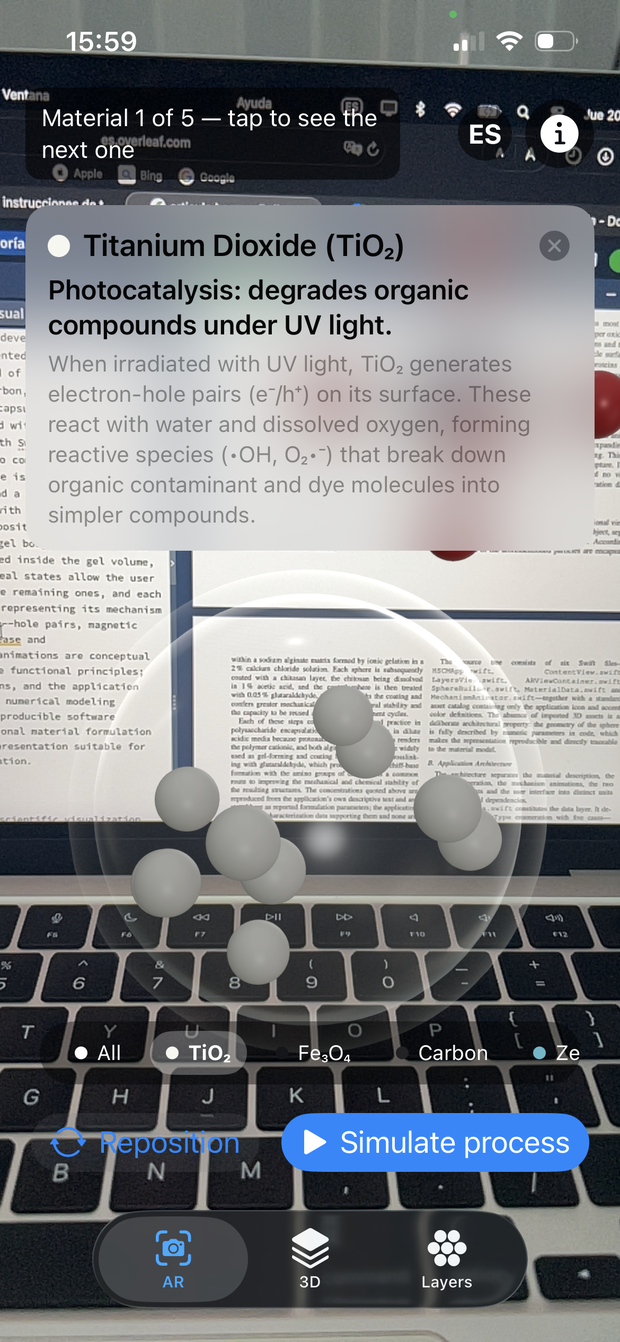
\includegraphics[width=0.20\linewidth]{2026_Augmented_Reality_Multifunctional_Hybrid_Materials/figs/hscm2_en.PNG}
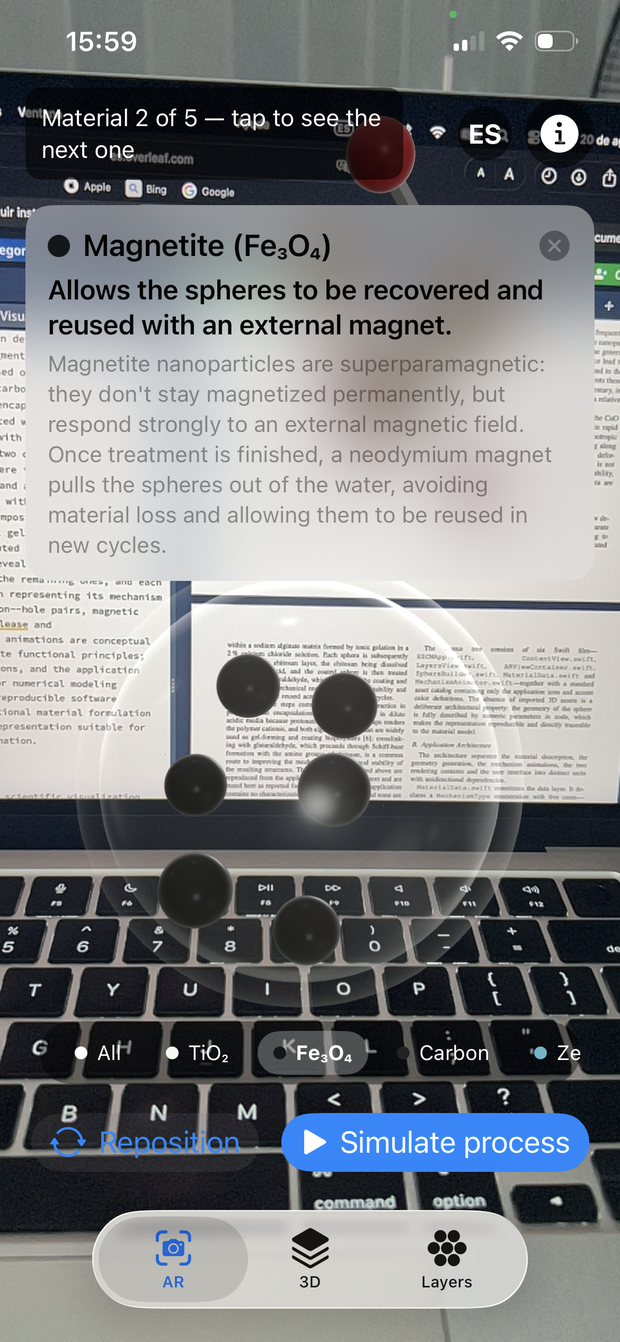
\includegraphics[width=0.20\linewidth]{2026_Augmented_Reality_Multifunctional_Hybrid_Materials/figs/hscm4_en.PNG}
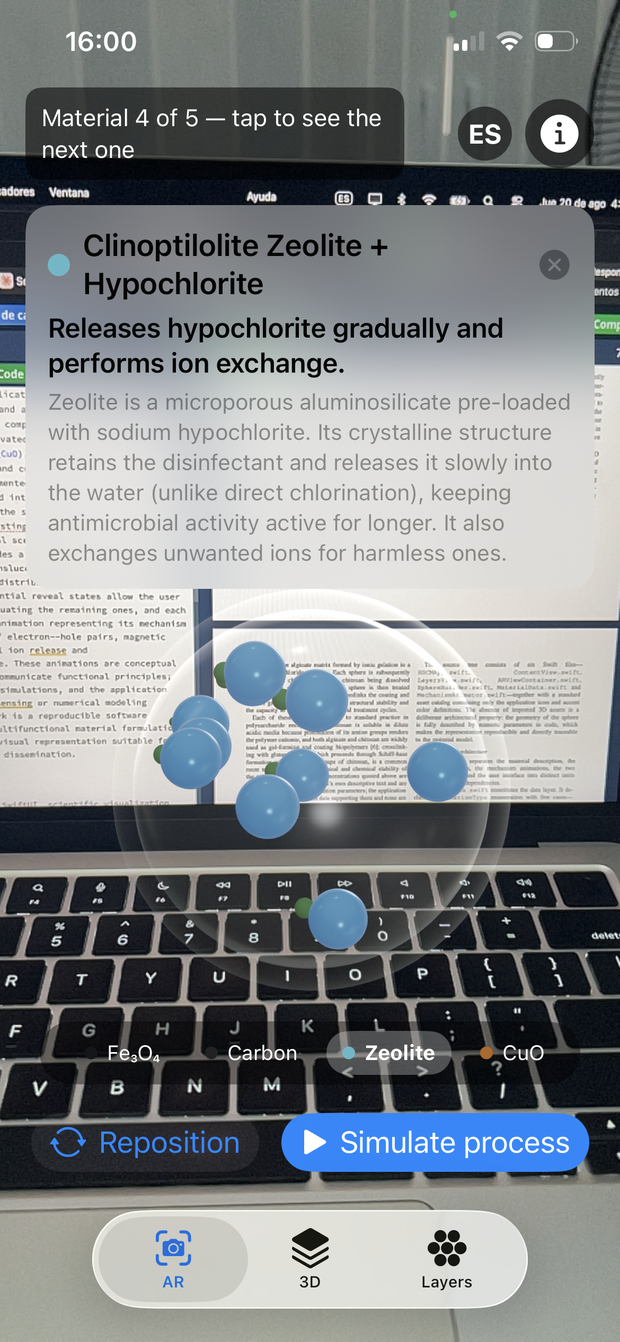
\includegraphics[width=0.20\linewidth]{2026_Augmented_Reality_Multifunctional_Hybrid_Materials/figs/hscm7_en.PNG}                                
\end{center}   
\end{columns}
\end{frame}


\begin{frame}{\citetitle{\EntradaBibtex} (4)}
\begin{columns}
% Column 1
\column{.4\linewidth}
Modo no-RA / entorno virtual
\begin{itemize}
\item La misma geometría 3D se presenta en una escena virtual.
\item Cámara con perspectiva fija.
\item Iluminación explícita para facilitar la inspección.
\end{itemize}
\column{.6\linewidth}
\begin{center}
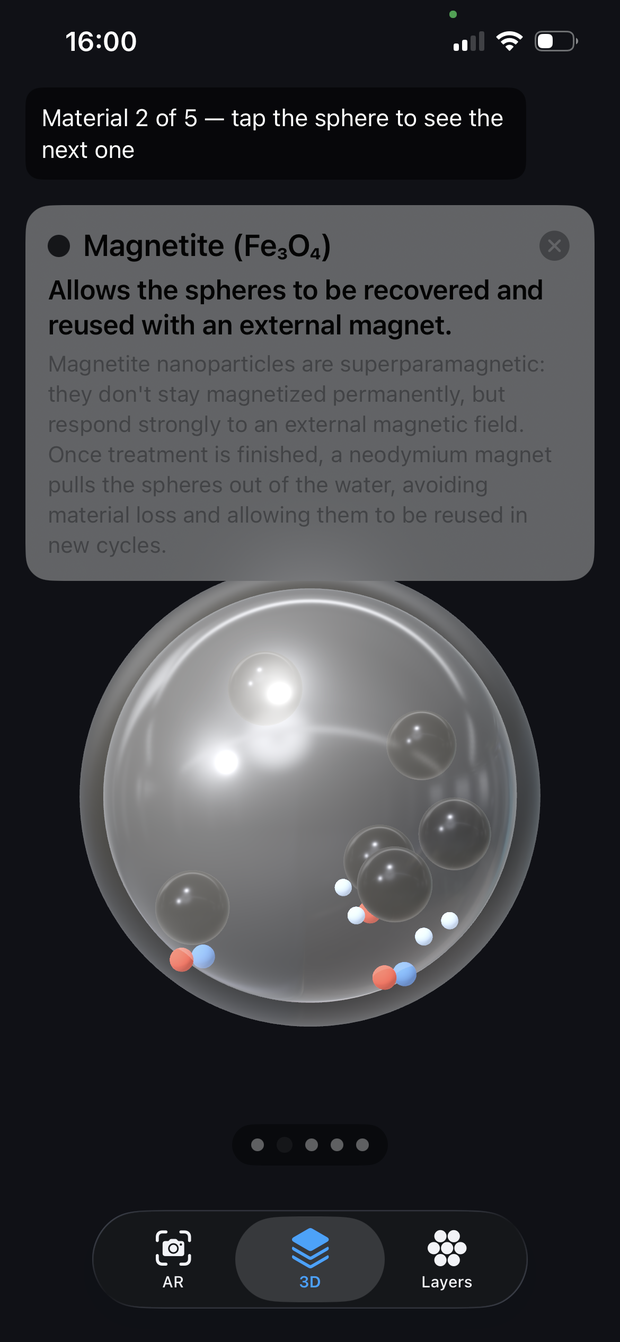
\includegraphics[width=0.20\linewidth]{2026_Augmented_Reality_Multifunctional_Hybrid_Materials/figs/hscm11_en.PNG}
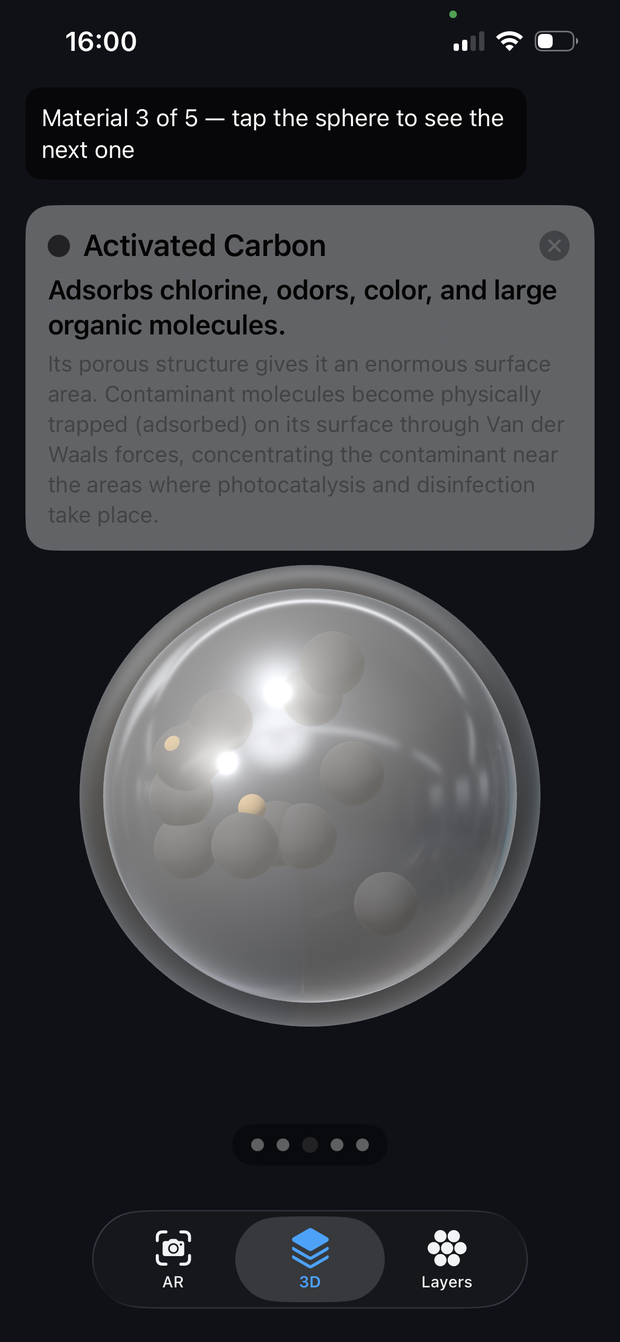
\includegraphics[width=0.20\linewidth]{2026_Augmented_Reality_Multifunctional_Hybrid_Materials/figs/hscm12_en.PNG}
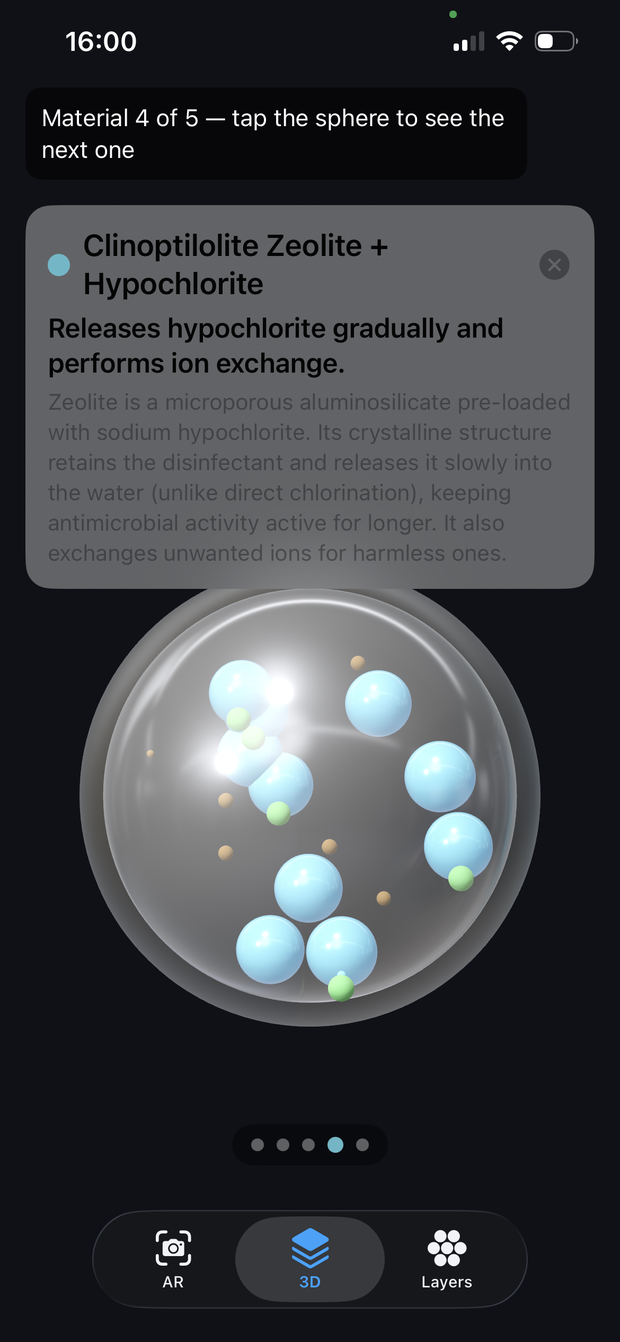
\includegraphics[width=0.20\linewidth]{2026_Augmented_Reality_Multifunctional_Hybrid_Materials/figs/hscm13_en.PNG}
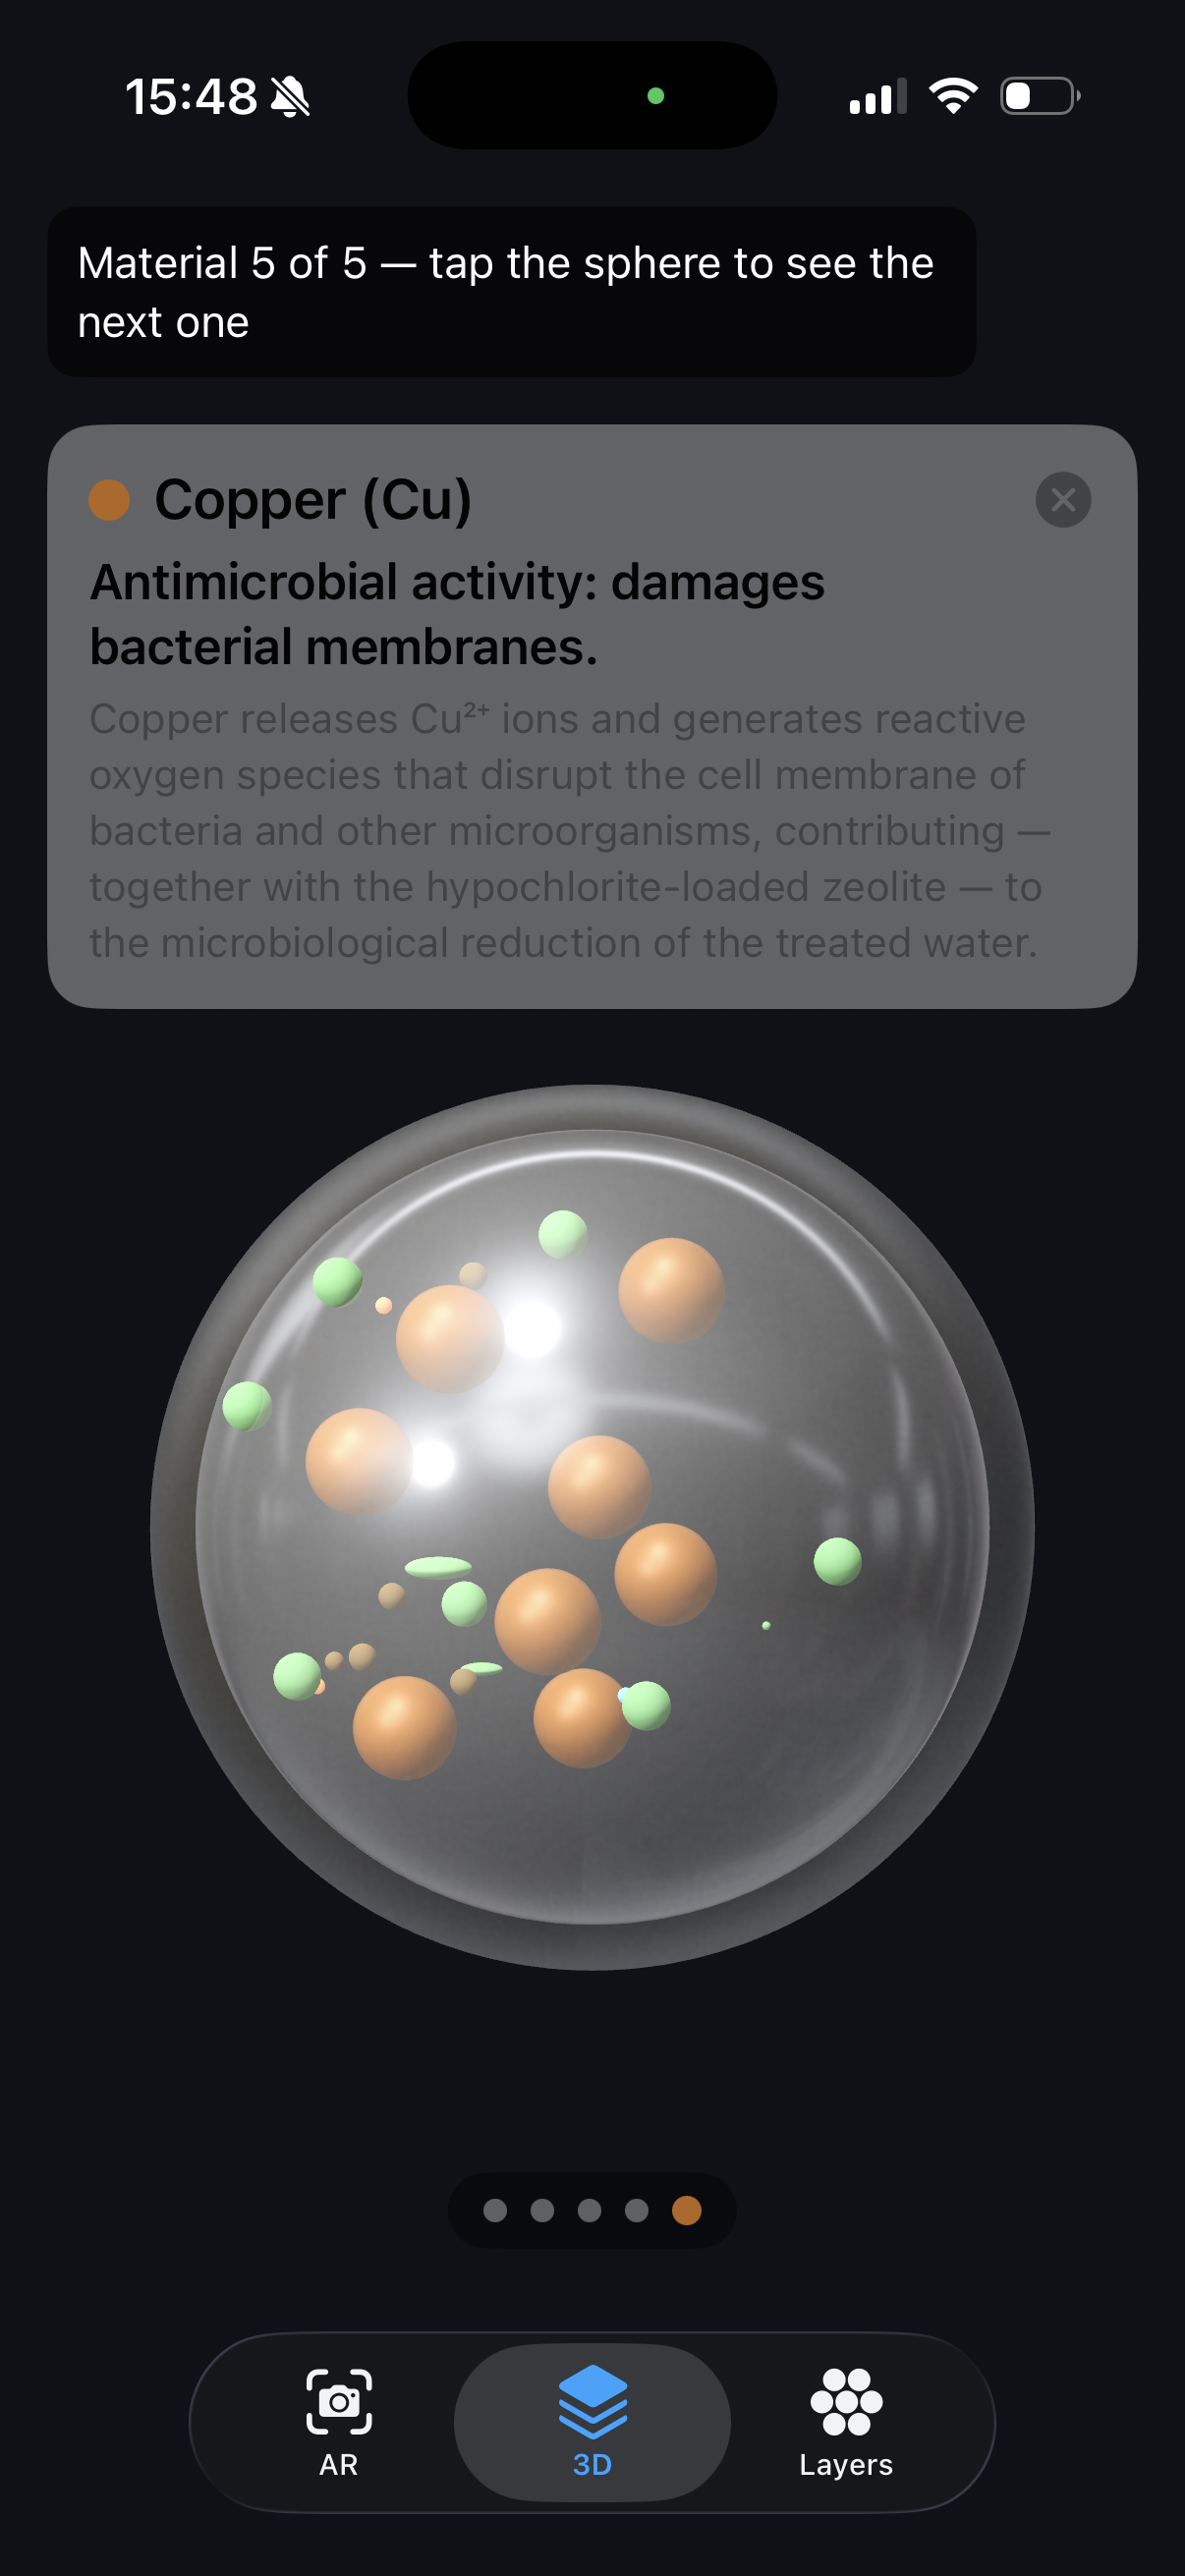
\includegraphics[width=0.20\linewidth]{2026_Augmented_Reality_Multifunctional_Hybrid_Materials/figs/hscm14_en_new.PNG}                                
\end{center}   
\end{columns}
\end{frame}


\begin{frame}{\citetitle{\EntradaBibtex} (5)}
Contribución principal
\begin{itemize}
\item Integración de RA + visualización 3D interactiva en una aplicación móvil.
\item Representación de la coexistencia espacial de múltiples fases dentro de un material híbrido.
\end{itemize}

Aplicaciones potenciales
\begin{itemize}
\item Educación: enseñanza de materiales y procesos químicos.
\item Comunicación científica: explicación de estructuras complejas.
\item Colaboración interdisciplinaria: interacción entre especialistas.
\item Ciencia de materiales: exploración de estructuras multifuncionales.
\end{itemize}
MHM-App demuestra el potencial de la RA y la visualización 3D móvil como herramientas para comprender, comunicar y explorar materiales multifuncionales complejos.
\end{frame}




\section{Conclusiones}

\begin{frame}
\frametitle{Relación entre IA y los proyectos presentados}
\framesubtitle{El smartphone como dispositivo de percepción}

\begin{block}{Cámara del smartphone como \textbf{sensor inteligente}}
\begin{itemize}
\item Reconocimiento de objetos de interes  (cromosomas, alimentos).
\item Detección de partes del cuerpo humano  (piel, manos, torso, cara).
\end{itemize}
\end{block}

\begin{block}{Procesamiento de datos de los sensores de smartphone}
\begin{itemize}
\item Acelerometros (clasificador de actividad).
\item WiFi (Detectar ubicación).
\end{itemize}
\end{block}


\begin{block}{Idea Aplicaciones didácticas/lúdicas para enriquecen la experiencia de usuario}
\begin{itemize}
\item Filtro de Jaguar/Aplicaciones de Realidad Aumentada.
\item Transportador Virtual/HSCM para materiales.
\end{itemize}

\end{block}


\end{frame}


\begin{frame}
\frametitle{¿Qué tienen en común estos proyectos?}

\framesubtitle{Una línea común: Inteligencia Artificial en el dispositivo}

\begin{center}

\begin{tikzpicture}[
    box/.style={
        draw,
        rounded corners,
        minimum width=3.0cm,
        minimum height=1.0cm,
        align=center,
        font=\small
    },
    arrow/.style={-{Latex}, very thick}
]

\node[box] (p) {
    \textbf{PERCEPCIÓN}\\
    Imágenes\\
    Video\\
    Gestos\\
    Sensores
};

\node[box, right=1cm of p] (i) {
    \textbf{INTELIGENCIA}\\
    Clasificación\\
    Detección\\
    Segmentación\\
    Predicción
};

\node[box, right=1cm of i] (in) {
    \textbf{INTERACCIÓN}\\
    RA\\
    Interfaces naturales\\
    Modelos 3D
};

\node[box, right=1cm of in] (a) {
    \textbf{APLICACIÓN}\\
    Educación\\
    Salud/deporte\\
    Cultura\\
    Seguridad
};

\draw[arrow] (p) -- (i);
\draw[arrow] (i) -- (in);
\draw[arrow] (in) -- (a);

\end{tikzpicture}

\end{center}

\vspace{0.35cm}

\begin{alertblock}{Conclusión}
Los proyectos comparten una arquitectura conceptual basada en
\textbf{percibir, interpretar e interactuar} utilizando recursos
computacionales disponibles en dispositivos móviles.
\end{alertblock}

\end{frame}

\begin{frame}[plain]
\begin{tikzpicture}[remember picture,overlay]

    % Fondo
    \fill[blue!8]
        (current page.south west)
        rectangle
        (current page.north east);

    % Elementos decorativos
    \fill[blue!75!black]
        ([xshift=-1.5cm,yshift=1.2cm]current page.south east)
        circle (3.2cm);

    \fill[cyan!65]
        ([xshift=0.8cm,yshift=-0.8cm]current page.north west)
        circle (2.1cm);

    \fill[orange!80]
        ([xshift=-2.0cm,yshift=-1.0cm]current page.north east)
        circle (0.35cm);

    % Texto principal
    \node[
        align=center,
        text=blue!75!black,
        font=\fontsize{42}{50}\selectfont\bfseries
    ] at ([yshift=0.4cm]current page.center)
    {¡Gracias!};

    % Línea decorativa
    \draw[cyan!70!blue,line width=2pt]
        ([xshift=-1.5cm,yshift=-0.5cm]current page.center)
        --
        ([xshift=1.5cm,yshift=-0.5cm]current page.center);

    % Mensaje final
    \node[
        align=center,
        text=black!70,
        font=\large
    ] at ([yshift=-1.2cm]current page.center)
    {¿Preguntas o comentarios? \\ mnunom@upv.edu.mx};

\end{tikzpicture}
\end{frame}




\end{document}


